\documentclass[12pt]{book}\usepackage[]{graphicx}\usepackage[]{color}
%% maxwidth is the original width if it is less than linewidth
%% otherwise use linewidth (to make sure the graphics do not exceed the margin)
\makeatletter
\def\maxwidth{ %
  \ifdim\Gin@nat@width>\linewidth
    \linewidth
  \else
    \Gin@nat@width
  \fi
}
\makeatother

\definecolor{fgcolor}{rgb}{0.345, 0.345, 0.345}
\newcommand{\hlnum}[1]{\textcolor[rgb]{0.686,0.059,0.569}{#1}}%
\newcommand{\hlstr}[1]{\textcolor[rgb]{0.192,0.494,0.8}{#1}}%
\newcommand{\hlcom}[1]{\textcolor[rgb]{0.678,0.584,0.686}{\textit{#1}}}%
\newcommand{\hlopt}[1]{\textcolor[rgb]{0,0,0}{#1}}%
\newcommand{\hlstd}[1]{\textcolor[rgb]{0.345,0.345,0.345}{#1}}%
\newcommand{\hlkwa}[1]{\textcolor[rgb]{0.161,0.373,0.58}{\textbf{#1}}}%
\newcommand{\hlkwb}[1]{\textcolor[rgb]{0.69,0.353,0.396}{#1}}%
\newcommand{\hlkwc}[1]{\textcolor[rgb]{0.333,0.667,0.333}{#1}}%
\newcommand{\hlkwd}[1]{\textcolor[rgb]{0.737,0.353,0.396}{\textbf{#1}}}%
\let\hlipl\hlkwb

\usepackage{framed}
\makeatletter
\newenvironment{kframe}{%
 \def\at@end@of@kframe{}%
 \ifinner\ifhmode%
  \def\at@end@of@kframe{\end{minipage}}%
  \begin{minipage}{\columnwidth}%
 \fi\fi%
 \def\FrameCommand##1{\hskip\@totalleftmargin \hskip-\fboxsep
 \colorbox{shadecolor}{##1}\hskip-\fboxsep
     % There is no \\@totalrightmargin, so:
     \hskip-\linewidth \hskip-\@totalleftmargin \hskip\columnwidth}%
 \MakeFramed {\advance\hsize-\width
   \@totalleftmargin\z@ \linewidth\hsize
   \@setminipage}}%
 {\par\unskip\endMakeFramed%
 \at@end@of@kframe}
\makeatother

\definecolor{shadecolor}{rgb}{.97, .97, .97}
\definecolor{messagecolor}{rgb}{0, 0, 0}
\definecolor{warningcolor}{rgb}{1, 0, 1}
\definecolor{errorcolor}{rgb}{1, 0, 0}
\newenvironment{knitrout}{}{} % an empty environment to be redefined in TeX

\usepackage{alltt}

\usepackage[hmargin=2cm,vmargin=2cm,headsep=0.5cm]{geometry}  

%% added by SV:
\usepackage{hyperref}
\hypersetup{a4paper=TRUE,ps2pdf=TRUE,colorlinks=TRUE,linkcolor=blue,anchorcolor=blue,filecolor=blue,pagecolor=blue,urlcolor=blue,citecolor=blue,bookmarksnumbered=true}
\usepackage{amsmath}
\usepackage{amssymb}
%\usepackage{apacite}

\usepackage{mathptmx}
\usepackage{helvet}
\usepackage{courier}
%
\usepackage{type1cm}         

\usepackage{makeidx}         % allows index generation
\usepackage{graphicx}        % standard LaTeX graphics tool
                             % when including figure files

\usepackage{mathtools}
\makeatletter
 
\newcommand{\explain}[2]{\underset{\mathclap{\overset{\uparrow}{#2}}}{#1}}
\newcommand{\explainup}[2]{\overset{\mathclap{\underset{\downarrow}{#2}}}{#1}}
 
\makeatother

%% taken from http://brunoj.wordpress.com/2009/10/08/latex-the-framed-minipage/
\newsavebox{\fmbox}
\newenvironment{fmpage}[1]
{\begin{lrbox}{\fmbox}\begin{minipage}{#1}}
{\end{minipage}\end{lrbox}\fbox{\usebox{\fmbox}}}


\hyphenation{distribu-tion}

% see the list of further useful packages
% in the Reference Guide

\makeindex             % used for the subject index
                       % please use the style svind.ist with
                       % your makeindex program

%%%%%%%%%%%%%%%%%%%%%%%%%%%%%%%%%%%%%%%%%%%%%%%%%%%%%%%%%%%%%%%%%%%%%

% NOTE:
% The line below defines the location of figures generated while compiling
% (This file will create this directory automatically, see code chunk
% ``init'' below. 
%\SweaveOpts{prefix.string=figures/lecturesfig}




\IfFileExists{upquote.sty}{\usepackage{upquote}}{}
\begin{document}


\title{An introduction to statistical data analysis (Winter 2018)\\ Lecture notes}
\author{Shravan Vasishth [vasishth@uni-potsdam.de]}
\date{Last edited: \today}
\maketitle

\frontmatter

\tableofcontents

\mainmatter





\chapter{What this course is about}

This is a graduate level course in linguistics that introduces statistical data analysis to people who have presumably never done any data analysis before. Only high school pre-calculus mathematics is presupposed, and even there not much is needed beyond basic math skills like addition, subtraction, multiplication, and division.

The goal of this course is to prepare students to understand and use the most commonly deployed statistical models in psycholinguistics. The course is designed to bring people to terms with the linear mixed model framework. We ignore ANOVA in this course because there is not enough time to cover it, and besides, ANOVA is now only a historical artefact of a pre-computing era (in my opinion). We also limit the discussion to two commonly used distributions: the binomial and normal distributions.

The most frequent question people tend to have in this class is: \textbf{why do I need to study all this stuff}? The short answer is that linguistics is now a heavily experimental science, and one cannot function in linguistics any more without at least a basic knowledge of statistics. 
Because time is short in this course, I decided to drastically limit the scope of the course, so that we cover only a small number of topics; these will be the most frequently used tools in linguistics.

By the end of the course you should know the following:

\begin{itemize}
\item \textbf{Basic} usage of the R language for data analysis.
\item Basic understanding of the logic of null hypothesis significance testing.
\item The meaning of confidence intervals, p-values, z- and t-values, Type I and II error, Type M, S error, Power. 
\item Linear models (including simple multiple regression), basic contrast coding for $2\times 2$ repeated measures designs.
%\item Basics of analysis of variance, including repeated measures anova.
\item Basics of fitting linear mixed models and presenting results.
\end{itemize}

Many people come to this course expecting to become experts in data analysis. No one course can achieve that. The present course should be seen as an introduction; for your own research problems, be prepared to study further.

\section{Quiz: Do you need this course?}

You should take this quiz on your own to decide whether you need this course. If you can answer (almost) all the questions correctly, you are in pretty good shape. If you made more than one mistake or don't know the answer to more than one question, you should probably do this course. The solutions are at the end of the book.

\textbf{Instructions}: choose only one answer by circling the relevant letter. If you don't know the answer, just leave the answer blank. 

\begin{enumerate}
\item Standard error is

\begin{enumerate}
\item[a] the standard deviation of the sample scores
\item[b] the standard deviation of the distribution of sample means
\item[c] the square root of the sample variance
\item[d] 2 times the standard deviation of sample scores
\end{enumerate}

\item
If we sum up the differences of each sample score from the sample's mean (average) we will always get

\begin{enumerate}
\item[a] a large number
\item[b] the number zero
\item[c] a different number each time, sometimes large, sometimes small
\item[d] the number one
\end{enumerate}

\item As sample size increases, the standard error of the sample should

\begin{enumerate}
\item[a]
increase
\item[b]
decrease
\item[c]
remain unchanged
\end{enumerate}

\item
The 95\% confidence interval tells you

\begin{enumerate}
\item[a]
that the probability is 95\% that the population mean is equal to the sample mean
\item[b]
that the sample mean lies within this interval with probability 95\%
\item[c]
that the population mean lies within this interval with probability 95\%
\item[d] 
none of the above
\end{enumerate}

\item
The 95\% confidence interval is roughly equal to 

\begin{enumerate}
\item[a]
 0.5 times the standard error
\item[b]
 1 times the standard error
\item[c]
1.5 times the standard error
\item[d]
2 times the standard error
\end{enumerate}

\item
The 95\% confidence interval is --- the 90\% confidence interval

\begin{enumerate}
\item[a]
wider than
\item[b]
narrower than
\item[c]
same as
\end{enumerate}

\item
A p-value is

\begin{enumerate}
\item[a]
the probability of the null hypothesis being true
\item[b]
the probability of the null hypothesis being false
\item[c]
the probability of the alternative hypothesis being true
\item[d]
the probability of getting the sample mean that you got (or a value more extreme) assuming the null hypothesis is true
\item[e]
the probability of getting the sample mean that you got (or a value less extreme) assuming the null hypothesis is true
\end{enumerate}

\item
If Type I error probability, alpha, is 0.05 in a t-test, then

\begin{enumerate}
\item[a]
we have a 5\% probability of rejecting the null hypothesis when it is actually true
\item[b]
we have a 95\% probability of rejecting the null hypothesis when it is actually true
\item[c]
we necessarily have low power
\item[d]
we necessarily have high power
\end{enumerate}

\item
Type II error probability is

\begin{enumerate}
\item[a]
the probability of accepting the null when it's true
\item[b]
the probability of accepting the null when it's false
\item[c]
the probability of rejecting the null when it's true
\item[d]
the probability of rejecting the null when it's false
\end{enumerate}

\item
When power increases
\begin{enumerate}
\item[a]
Type II error probability decreases
\item[b]
Type II error probability increases
\item[c]
Type II error probability remains unchanged
\end{enumerate}

\item
If we compare two means from two samples, and the p$>$0.05 (p is greater than 0.05), we can conclude 

\begin{enumerate}
\item[a]
that the two samples comes from two populations with different means
\item[b]
 that the two samples comes from two populations with identical means
\item[c]
that we don't know whether two samples comes from two populations with identical means or not
\end{enumerate}
\end{enumerate}

\section{How to survive and perhaps even enjoy this course}

I have been teaching this course for several years now, and one reaction that I get quite often is fear, panic, and even anger.
A common reaction is: Why do I have to learn all this? How can I do all this programming? And so on. 

If you have such questions popping up in your mind, you have to stop and consider a few things before continuing with this course.  
Linguistics at Potsdam is a very empirically driven program. It is impossible to get through a master's degree in linguistics without coming into contact with data, even in formerly non-experimental disciplines like syntax or semantics. If you are at Potsdam, you are automatically committed to an empirically driven education. 

More broadly, there is a widespread misunderstanding that statistics is something that can be outsourced to a statistician. It's true that if you have a non-standard statistical problem you probably need to talk to a professional. But for the kinds of methods used in linguistics, you are personally responsible for the analyses you do, and so you are going to have to learn something about the methods. Many scientists do not understand that in experimental science, the statistics is inseparable from the science, it is not an unnecessary add-on. This is because our statistical inferences inform our scientific conclusions, and if the inferences are wrong, so will be the conclusions. I will provide some examples in this course.

In order to pass this course, you have to understand that \textbf{you have to read the lecture notes}, and that
it is not enough to just passively read these lecture notes. You have to play with the ideas by asking yourself questions like ``what would happen if\dots'', and then check the answer right there using R. That's the whole point of this approach to teaching statistics, that you can verify what happens under repeated sampling. There is no point in memorizing formulas; focus on developing understanding. The concepts presented here require nothing more than middle or high school (pre-calculus) mathematics. The ideas are not easy to understand, but simulation is a great way to develop a deeper understanding of the logic of statistical theory.

Many students students worry that they might make a mistake.  It is normal to make mistakes. One should use mistakes as a learning tool. A mistake is a very useful message telling you that you need to think about the material again. A good book that talks about how to learn and solve problems is \textit{The five elements of effective thinking}. I highly recommend this book as preparation for the present course.

\section{Installing R and learning basic usage}

You should google the word CRAN and RStudio and install R and RStudio on your machine. We will explain basic R uage in class; also see the introductory notes on using R released on Moodle.
You should spend some time on the CRAN website looking at the information available on R there. Look especially at the section called Contributed (navigation panel on the left on the main page).

A good first introduction to R for non-programmers is: https://rstudio-education.github.io/hopr/

%%SDSM


\chapter{The logic of (hypothetical) repeated sampling}

\section{Random variables}

A random variable $X$ is a function $X : S \rightarrow \mathbb{R}$ that associates to each outcome
$\omega \in S$ exactly one number $X(\omega) = x$.

$S_X$ is all the $x$'s (all the possible values of X, the support of X). I.e., $x \in S_X$.

\subsection{Example of a discrete random variable}

Imagine tossing a coin repeatedly until you get a heads. What we are measuring here is the number of times we have to toss the coin to get a heads.

\begin{itemize}
	\item $X: \omega \rightarrow x$
	\item $\omega$: H, TH, TTH,\dots (infinite)
	\item $x=0,1,2,\dots; x \in S_X$
\end{itemize}

Every discrete random variable X has associated with it a \textbf{probability mass  function (pmf)}. 


\begin{equation}
p_X : S_X \rightarrow [0, 1] 
\end{equation}

defined by

\begin{equation}
p_X(x) = P(X(\omega) = x), x \in S_X
 \end{equation}

In addition to the pmf, a discrete random variable also has associated with it a cumulative distribution function $F(\cdot)$, which allows you to ask questions like: what is the probability of obtaining a value $x$ or some value less than it: $Prob(X\leq x)$. 

\subsection{Example of a continuous random variable}

Imagine measuring the reading time at a particular word in a sentence. Here, we are measuring a continuous random variable that has minimum value 0.  Such a random variable has a probability density function and a cumulative distribution function associated with it. An example we will consider next is a random variable that has the normal distribution as its pdf.


\section{The normal distribution}

A typical situation in linguistic research involves collecting reading times or reaction times in a particular experiment to answer a specific research question.   For example, I might want to know whether subject relatives (SRs) are read faster than object relatives (ORs) in a population of speakers (say 
English speakers). To find this out, I would get randomly selected participants to read SRs and ORs; the details of experiment design will be discussed later. Right now, all that matters is that if I do such an experiment, I will get a difference in reading times between SRs and ORs for each participant. Suppose I have 100 participants, and I know the difference in OR vs SR reading times, in seconds. We can simulate this situation in R. We could have 100 data points, each representing a difference in means between subject and object relatives seen by each subject (synonymous here with participant). 

\begin{knitrout}
\definecolor{shadecolor}{rgb}{0.969, 0.969, 0.969}\color{fgcolor}\begin{kframe}
\begin{alltt}
\hlstd{x}\hlkwb{<-}\hlkwd{rnorm}\hlstd{(}\hlnum{100}\hlstd{)}
\hlkwd{head}\hlstd{(x)}
\end{alltt}
\begin{verbatim}
## [1]  0.5446905  0.3039760  0.3630976 -0.7654192 -0.4456920 -1.6158883
\end{verbatim}
\end{kframe}
\end{knitrout}

This is a (simulated) \textbf{sample}; we could have taken a different sample from the population of English speakers. You can simulate that by running the above code again.

The sample we did take comes from a \textbf{population} of speakers. Note that, for theoretical reasons we won't go into, it is important to take a \textbf{random sample}. In practice, this is not really the case---we just take the university students who are willing to come do the experiment. This is likely to introduce a bias in our results, in that the result is probably going to not be representative of the population. This is a limitation of the way we do experiments in psycholinguistics and psychology.

As mentioned above, each value in the above simulated sample represents one participant's response. A positive value means that the OR was read more slowly than the SR. If we plot the distribution of this sample's values, then we will see that it has roughly a ``bell-shaped distribution'':

\begin{figure}
\begin{knitrout}
\definecolor{shadecolor}{rgb}{0.969, 0.969, 0.969}\color{fgcolor}\begin{kframe}
\begin{alltt}
\hlcom{## plot density histogram:}
\hlkwd{hist}\hlstd{(x,}\hlkwc{freq}\hlstd{=F)}
\end{alltt}
\end{kframe}
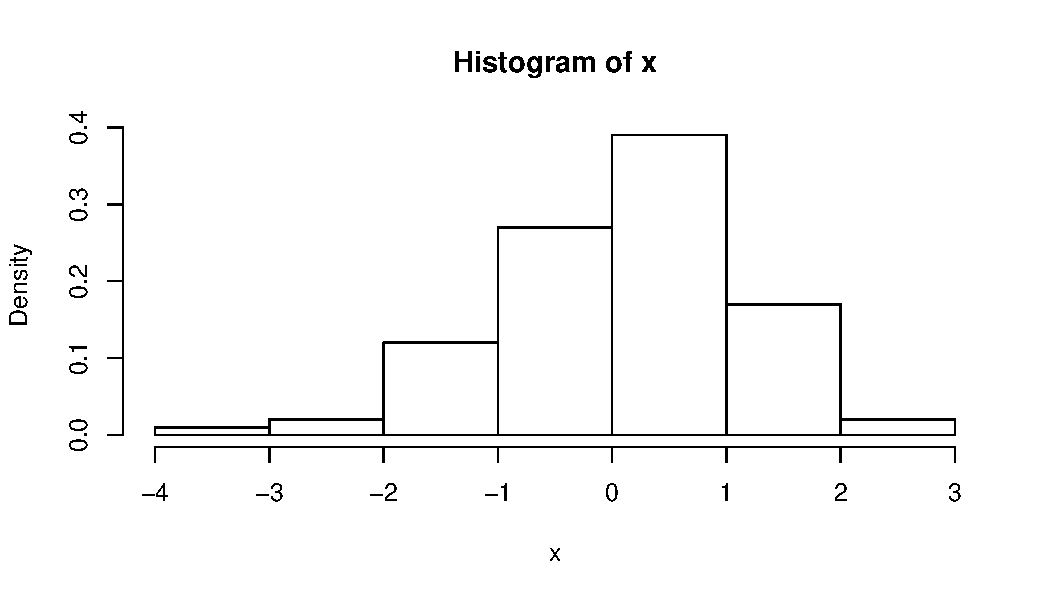
\includegraphics[width=\maxwidth]{figure/unnamed-chunk-4-1} 

\end{knitrout}
\caption{A histogram of the sample data.}\label{hist1}
\end{figure}
Notice that most of the values are centered around 0, some are as big as 3, and some are as small as -3. 

It turns out that a lot of very convenient theory can be built around this distribution. Since normal distribution theory is so fundamental to what we do in linguistics, I am going to focus on better understanding this one distribution.

The following function is defined as the normal density function:

\begin{equation}
f(x,\mu,\sigma) = \frac{1}{\sigma \sqrt{2 \pi}} \exp^{-((x - \mu)^2/2 \sigma^2)}
\end{equation}

Given a range of values for $x$, and specific values for $\mu$, and $\sigma$, we can
plot the result of applying this function. 
Since the function is defined by two values or \textbf{parameters}, we can write it in shorthand as follows:
$N(\mu,\sigma)$, i.e., a normal distribution with some mean and some standard deviation. Statisticians usually write $N(\mu,\sigma^2)$, i.e., they use the variance $\sigma^2$ rather than the standard deviation $\sigma$; but we will ignore the statisticians' convention in this course, because in R we define the density function in terms of standard deviation. (But you should keep in mind that statisticians tend to define the normal distribution in terms of variance.)

We can define the probability density function in R as follows, setting mu and sigma to 0 and 1 respectively, for convenience (you could have set it to anything):

\begin{knitrout}
\definecolor{shadecolor}{rgb}{0.969, 0.969, 0.969}\color{fgcolor}\begin{kframe}
\begin{alltt}
\hlcom{## mean and sigma set at 0 and 1 by default:}
\hlstd{normal.density.function} \hlkwb{<-} \hlkwa{function}\hlstd{(}\hlkwc{x}\hlstd{,}\hlkwc{mu}\hlstd{=}\hlnum{0}\hlstd{,}\hlkwc{sigma}\hlstd{=}\hlnum{1}\hlstd{)\{}
  \hlnum{1}\hlopt{/}\hlstd{(}\hlkwd{sqrt}\hlstd{(}\hlnum{2}\hlopt{*}\hlstd{pi)}\hlopt{*}\hlstd{sigma)}\hlopt{*}\hlkwd{exp}\hlstd{(}\hlopt{-}\hlstd{((x} \hlopt{-} \hlstd{mu)}\hlopt{^}\hlnum{2}\hlopt{/}\hlstd{(}\hlnum{2}\hlopt{*}\hlstd{sigma}\hlopt{^}\hlnum{2}\hlstd{)))\}}
\end{alltt}
\end{kframe}
\end{knitrout}

You can plot the shape of this distribution using the following command:

\begin{verbatim}
plot(function(x) normal.density.function(x), -3, 3,
      main = "Normal density function",ylim=c(0,.4),
              ylab="density",xlab="X")
\end{verbatim}

\begin{figure}
\begin{knitrout}
\definecolor{shadecolor}{rgb}{0.969, 0.969, 0.969}\color{fgcolor}
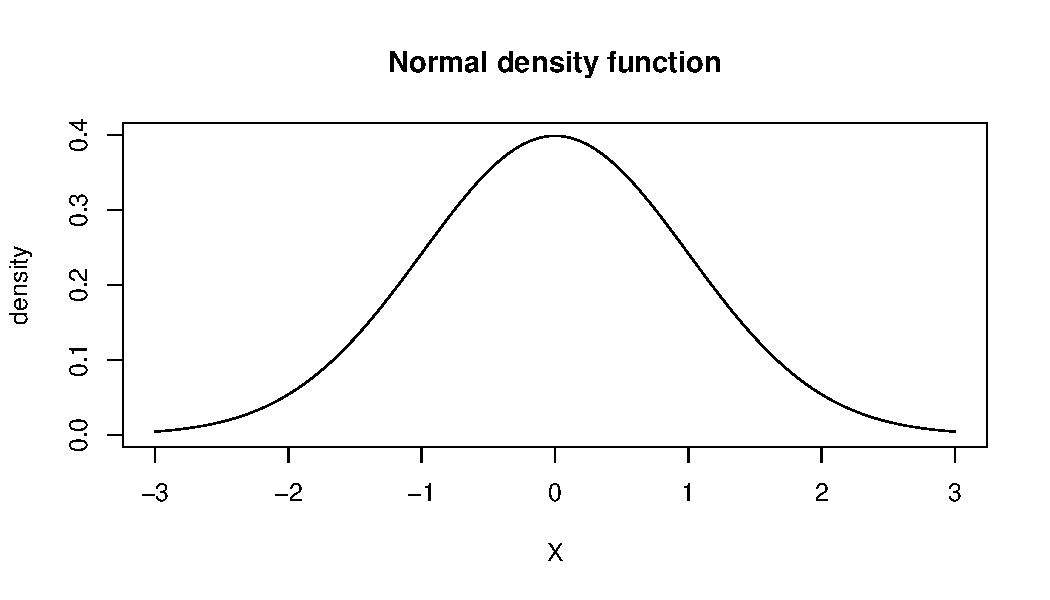
\includegraphics[width=\maxwidth]{figure/unnamed-chunk-6-1} 

\end{knitrout}
\caption{Plotting the normal distribution.}\label{norm1}
\end{figure}

R has a built-in function, \texttt{dnorm} that does the job of the function we defined above; we could just have used that built-in function:

\begin{knitrout}
\definecolor{shadecolor}{rgb}{0.969, 0.969, 0.969}\color{fgcolor}\begin{kframe}
\begin{alltt}
\hlkwd{plot}\hlstd{(}\hlkwa{function}\hlstd{(}\hlkwc{x}\hlstd{)} \hlkwd{dnorm}\hlstd{(x),} \hlopt{-}\hlnum{3}\hlstd{,} \hlnum{3}\hlstd{,}
      \hlkwc{main} \hlstd{=} \hlstr{"Normal density"}\hlstd{,}\hlkwc{ylim}\hlstd{=}\hlkwd{c}\hlstd{(}\hlnum{0}\hlstd{,}\hlnum{.4}\hlstd{),}
              \hlkwc{ylab}\hlstd{=}\hlstr{"density"}\hlstd{,}\hlkwc{xlab}\hlstd{=}\hlstr{"X"}\hlstd{)}
\end{alltt}
\end{kframe}
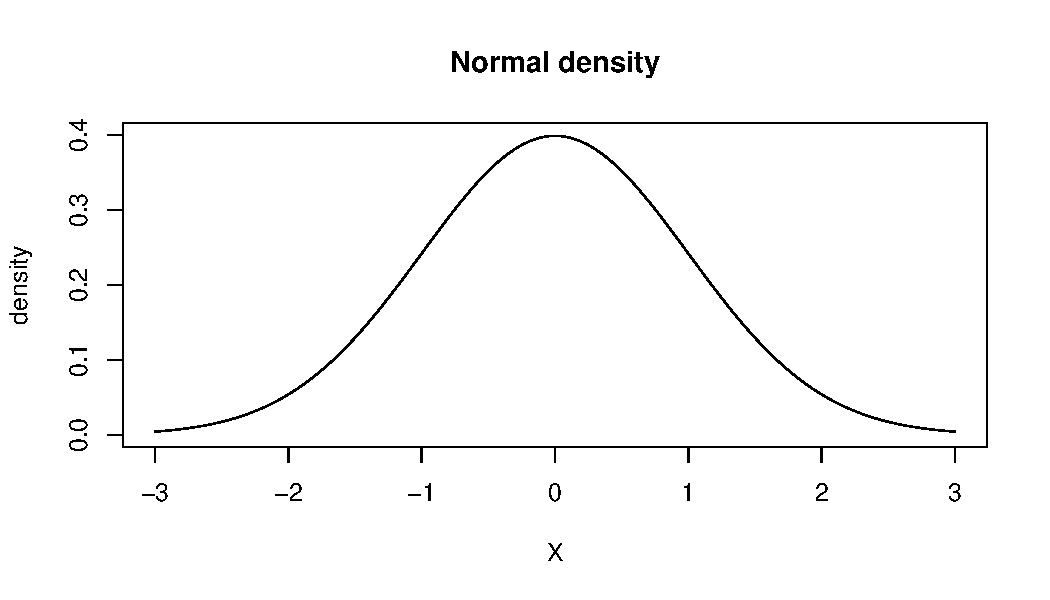
\includegraphics[width=\maxwidth]{figure/unnamed-chunk-7-1} 

\end{knitrout}

One important property of this function is that it stretches from -Infinity to +Infinity. We don't display this on the plot, hopefully it is obvious why not. Another important property is that it represents the probability of each of the x-axis values, and so the total probability of all possible values, stretching from all the way from -Infinity to +Infinity will be 1. You can calculate the total probability by summing up all the probabilities of all possible values. The function \texttt{integrate} does that summation for you:

\begin{knitrout}
\definecolor{shadecolor}{rgb}{0.969, 0.969, 0.969}\color{fgcolor}\begin{kframe}
\begin{alltt}
\hlkwd{integrate}\hlstd{(}\hlkwa{function}\hlstd{(}\hlkwc{x}\hlstd{)} \hlkwd{dnorm}\hlstd{(x,} \hlkwc{mean} \hlstd{=} \hlnum{0}\hlstd{,} \hlkwc{sd} \hlstd{=} \hlnum{1}\hlstd{),} \hlopt{-}\hlnum{Inf}\hlstd{,} \hlopt{+}\hlnum{Inf}\hlstd{)}
\end{alltt}
\begin{verbatim}
## 1 with absolute error < 9.4e-05
\end{verbatim}
\end{kframe}
\end{knitrout}

This will be our only brush with calculus in this course. The key point here is that it allows us to calculate the area under the curve given any lower and upper bound. For example, I could calculate the area under the curve between -2 and +2:

\begin{knitrout}
\definecolor{shadecolor}{rgb}{0.969, 0.969, 0.969}\color{fgcolor}\begin{kframe}
\begin{alltt}
\hlkwd{integrate}\hlstd{(}\hlkwa{function}\hlstd{(}\hlkwc{x}\hlstd{)} \hlkwd{dnorm}\hlstd{(x,} \hlkwc{mean} \hlstd{=} \hlnum{0}\hlstd{,} \hlkwc{sd} \hlstd{=} \hlnum{1}\hlstd{),} \hlopt{-}\hlnum{2}\hlstd{,} \hlopt{+}\hlnum{2}\hlstd{)}
\end{alltt}
\begin{verbatim}
## 0.9544997 with absolute error < 1.8e-11
\end{verbatim}
\end{kframe}
\end{knitrout}

Why am I talking about calculating the area under the curve? It turns out we need this capability a lot in statistical data analysis, as you are about to discover in this lecture. 

\section{The area under the curve in a normal distribution}

We begin by establishing a fundamental fact about any normal
distribution: 95\% of the probability lies within approximately 2 standard deviations (SDs) from the
mean. If we sum the area under these curves, between 2 SD below
the mean and 2 SD above the mean, we find the following areas, which
correspond to the amount of probability within these bounds. 

We can display this fact graphically (see Figure~\ref{fig:normal2SD}):



\begin{figure}[!htbp]
  \centering
\begin{knitrout}
\definecolor{shadecolor}{rgb}{0.969, 0.969, 0.969}\color{fgcolor}
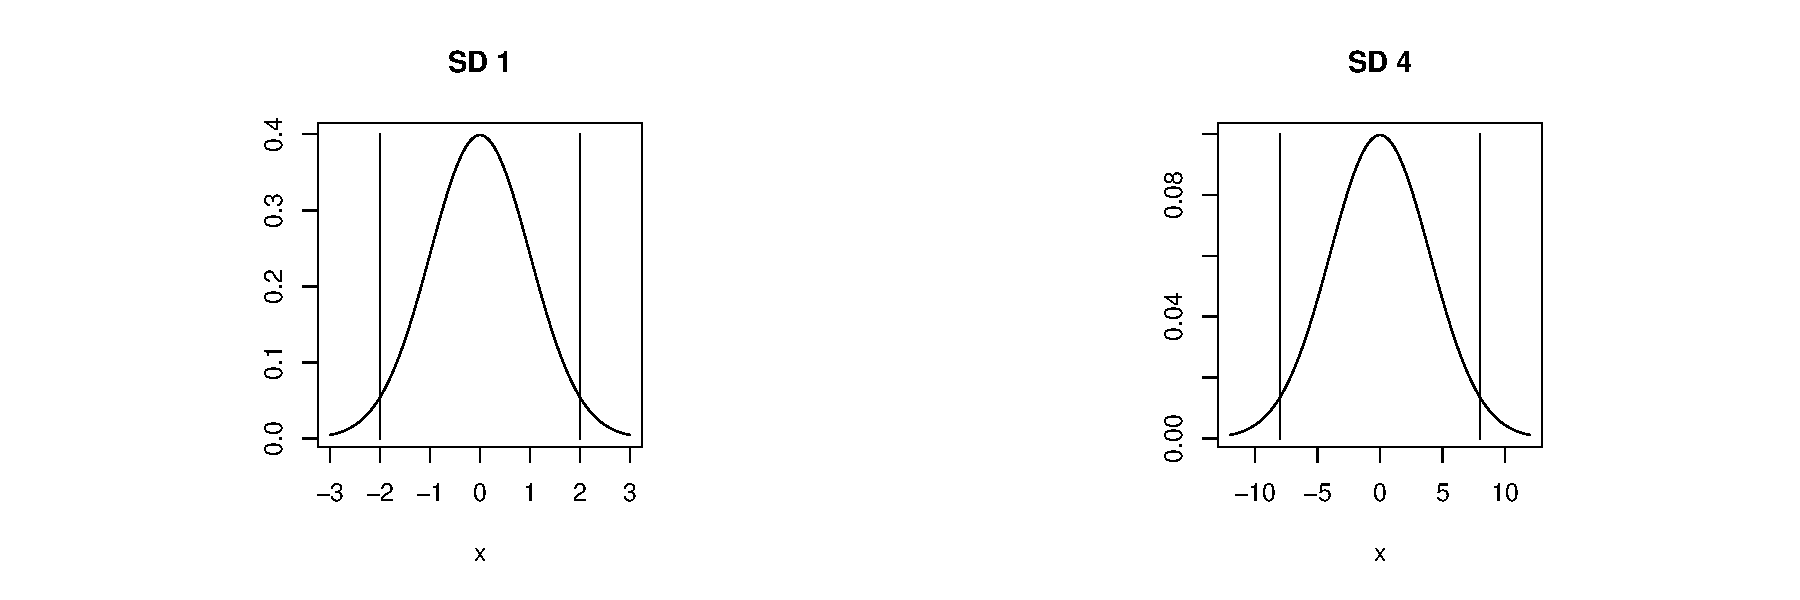
\includegraphics[width=\maxwidth]{figure/unnamed-chunk-10-1} 

\end{knitrout}
  \caption{Two normal distributions with SD $=1$ (left), SD $=4$ (right). The lines delimit the region 2 SD from the mean in each case.}
  \label{fig:normal2SD}
\end{figure}

There is a built-in R function, \texttt{pnorm}, for computing probabilities within a range; (so we don't really need the integrate function, I just used it initially to show that we are really doing a summation over continuous values). Here are some examples of \texttt{pnorm} in action. Here, we use the default values of \texttt{pnorm} for mean and standard deviation, but you could have had any mean or standard deviation: 

\begin{knitrout}
\definecolor{shadecolor}{rgb}{0.969, 0.969, 0.969}\color{fgcolor}\begin{kframe}
\begin{alltt}
\hlcom{## Prob. of getting 2 or less:}
\hlkwd{pnorm}\hlstd{(}\hlnum{2}\hlstd{)}
\end{alltt}
\begin{verbatim}
## [1] 0.9772499
\end{verbatim}
\begin{alltt}
\hlcom{## Prob. of getting more than 2:}
\hlnum{1}\hlopt{-}\hlkwd{pnorm}\hlstd{(}\hlnum{2}\hlstd{)}
\end{alltt}
\begin{verbatim}
## [1] 0.02275013
\end{verbatim}
\begin{alltt}
\hlcom{## Prob. of getting -2 or less:}
\hlkwd{pnorm}\hlstd{(}\hlopt{-}\hlnum{2}\hlstd{)}
\end{alltt}
\begin{verbatim}
## [1] 0.02275013
\end{verbatim}
\begin{alltt}
\hlcom{## Prob. of being between -2 and 2:}
\hlkwd{pnorm}\hlstd{(}\hlnum{2}\hlstd{)}\hlopt{-}\hlkwd{pnorm}\hlstd{(}\hlopt{-}\hlnum{2}\hlstd{)}
\end{alltt}
\begin{verbatim}
## [1] 0.9544997
\end{verbatim}
\end{kframe}
\end{knitrout}

You will sometimes need to know the following: given a normal distribution with a particular mean and standard deviation, what is the boundary marking x\% of the area under the curve (usually centered around the mean value). For example, 
the command \texttt{pnorm(2)-pnorm(-2)} gives us the area between -2 and 2 in a normal distribution with mean 0 and sd=1, and the area is  (I will freely switch between percentages and proportions for probability; don't get confused!). Suppose we only knew the area (probability) that we want to have under the curve, and want to know the bounds  that mark that area.
We actually know that the bounds are -2 and 2 here, but we will pretend we don't know and need to find this out.
How to do this?
The total area under the curve is 1. We want the lower and upper bounds for the area 
0.9545. This means that

\begin{equation}
1-0.9545= 0.0455
\end{equation}

\noindent 
is the area outside the (as yet unknown) bounds. Since the normal density curve is symmetrical, that means that each of the two sides outside the boundaries we want to discover has area 

\begin{equation}
\frac{0.0455}{2}=0.02275
\end{equation}

So: there is some lower bound with area 0.02275 to the \textbf{left} of it (i.e., in the lower tail), and some upper bound with area 0.02275 to the \textbf{right} of it (i.e., in the upper tail). We are pretending right now that we don't know that lower=-2 and upper=2; we are engaging in this pretence because we will be in situations soon where we don't know these values and have to discover them given some probability range. R allows you to ask: ``what is the bound, for a given distribution, such that the probability to the left of it is some value p1, or what is the bound such that the probability to the right of it is some value p2?'' 
The function that gives this answer is called \texttt{qnorm}, and here is how we can use to answer our current question:

\begin{knitrout}
\definecolor{shadecolor}{rgb}{0.969, 0.969, 0.969}\color{fgcolor}\begin{kframe}
\begin{alltt}
\hlcom{## figure out area between the unknown bounds:}
\hlstd{prob}\hlkwb{<-}\hlkwd{round}\hlstd{(}\hlkwd{pnorm}\hlstd{(}\hlnum{2}\hlstd{)}\hlopt{-}\hlkwd{pnorm}\hlstd{(}\hlopt{-}\hlnum{2}\hlstd{),}\hlkwc{digits}\hlstd{=}\hlnum{4}\hlstd{)}
\hlcom{## figure out lower bound:}
\hlstd{(lower}\hlkwb{<-}\hlkwd{qnorm}\hlstd{((}\hlnum{1}\hlopt{-}\hlstd{prob)}\hlopt{/}\hlnum{2}\hlstd{,}\hlkwc{mean}\hlstd{=}\hlnum{0}\hlstd{,}\hlkwc{sd}\hlstd{=}\hlnum{1}\hlstd{,}\hlkwc{lower.tail}\hlstd{=T))}
\end{alltt}
\begin{verbatim}
## [1] -2.000002
\end{verbatim}
\begin{alltt}
\hlcom{## figure out upper bound:}
\hlstd{(upper}\hlkwb{<-}\hlkwd{qnorm}\hlstd{((}\hlnum{1}\hlopt{-}\hlstd{prob)}\hlopt{/}\hlnum{2}\hlstd{,}\hlkwc{mean}\hlstd{=}\hlnum{0}\hlstd{,}\hlkwc{sd}\hlstd{=}\hlnum{1}\hlstd{,}\hlkwc{lower.tail}\hlstd{=F))}
\end{alltt}
\begin{verbatim}
## [1] 2.000002
\end{verbatim}
\end{kframe}
\end{knitrout}

And so we discover what we expected: the lower bound is -2 and the upper bound is 2.
It \textbf{always} helps to visualize what we are doing:

\begin{knitrout}
\definecolor{shadecolor}{rgb}{0.969, 0.969, 0.969}\color{fgcolor}\begin{kframe}
\begin{alltt}
\hlkwd{plot}\hlstd{(}\hlkwa{function}\hlstd{(}\hlkwc{x}\hlstd{)} \hlkwd{dnorm}\hlstd{(x,} \hlkwc{mean} \hlstd{=} \hlnum{0}\hlstd{,} \hlkwc{sd} \hlstd{=} \hlnum{1}\hlstd{),}
\hlkwc{xlim}\hlstd{=}\hlkwd{c}\hlstd{(}\hlopt{-}\hlnum{4}\hlstd{,} \hlnum{4}\hlstd{),}\hlkwc{main}\hlstd{=}\hlstr{"mean 1, SD 1"}\hlstd{,}\hlkwc{xlab}\hlstd{=}\hlstr{"x"}\hlstd{,}\hlkwc{ylab}\hlstd{=}\hlstr{""}\hlstd{,}\hlkwc{cex}\hlstd{=}\hlnum{2}\hlstd{)}
\hlkwd{segments}\hlstd{(}\hlopt{-}\hlnum{2}\hlstd{,} \hlnum{0}\hlstd{,} \hlopt{-}\hlnum{2}\hlstd{,} \hlnum{0.1}\hlstd{)}
\hlkwd{segments}\hlstd{(}\hlnum{2}\hlstd{,} \hlnum{0}\hlstd{,} \hlnum{2}\hlstd{,} \hlnum{0.1}\hlstd{)}
\hlkwd{text}\hlstd{(}\hlnum{0}\hlstd{,}\hlnum{.05}\hlstd{,}\hlstr{"probability=0.9545"}\hlstd{)}
\hlkwd{text}\hlstd{(}\hlopt{-}\hlnum{3}\hlstd{,}\hlnum{.05}\hlstd{,}\hlstr{"lower tail"}\hlstd{)}
\hlkwd{text}\hlstd{(}\hlopt{-}\hlnum{3}\hlstd{,}\hlnum{.005}\hlstd{,}\hlstr{"probability=0.02275"}\hlstd{)}
\hlkwd{text}\hlstd{(}\hlnum{3}\hlstd{,}\hlnum{.05}\hlstd{,}\hlstr{"upper tail"}\hlstd{)}
\hlkwd{text}\hlstd{(}\hlnum{3}\hlstd{,}\hlnum{.005}\hlstd{,}\hlstr{"probability=0.02275"}\hlstd{)}
\end{alltt}
\end{kframe}
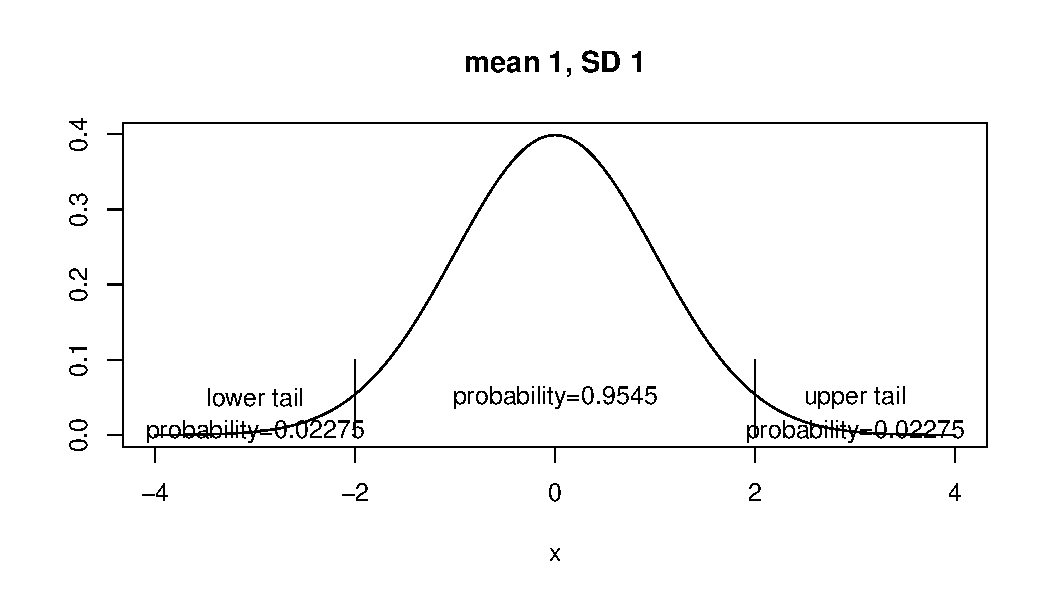
\includegraphics[width=\maxwidth]{figure/unnamed-chunk-13-1} 

\end{knitrout}

The skills we just learnt give us tremendous capability, as you will see in the rest of this chapter.

\section{Repeated sampling}

Suppose now that we have a population of people and that we know the age
of each individual; let us assume also that distribution of the ages
is approximately normal.
Finally, let us also suppose that we know that mean age of the
population is 60 years and the population SD is 4 years.

Now suppose that we \textbf{repeatedly} sample from this population: we take
samples of 40, a total of 1000 times; and we calculate the mean $\bar{x}$ each time
we take a sample. After taking 1000 samples, we have 1000 means; if we
plot the distribution of these means, we have the \textbf{sampling
distribution of the sample mean}.

\begin{knitrout}
\definecolor{shadecolor}{rgb}{0.969, 0.969, 0.969}\color{fgcolor}\begin{kframe}
\begin{alltt}
\hlcom{#1000 samples of 40 taken repeatedly:}
\hlstd{sample.means} \hlkwb{<-} \hlkwd{rep}\hlstd{(}\hlnum{NA}\hlstd{,}\hlnum{1000}\hlstd{)}
\hlkwa{for}\hlstd{(i} \hlkwa{in} \hlnum{1}\hlopt{:}\hlnum{1000}\hlstd{)\{}
  \hlstd{sample.40} \hlkwb{<-} \hlkwd{rnorm}\hlstd{(}\hlnum{40}\hlstd{,}\hlkwc{mean}\hlstd{=}\hlnum{60}\hlstd{,}\hlkwc{sd}\hlstd{=}\hlnum{4}\hlstd{)}
  \hlstd{sample.means[i]} \hlkwb{<-} \hlkwd{mean}\hlstd{(sample.40)}
\hlstd{\}}
\end{alltt}
\end{kframe}
\end{knitrout}

We can calculate the mean and standard deviation of this sampling distribution:

\begin{knitrout}
\definecolor{shadecolor}{rgb}{0.969, 0.969, 0.969}\color{fgcolor}\begin{kframe}
\begin{alltt}
\hlstd{means40}\hlkwb{<-}\hlkwd{mean}\hlstd{(sample.means)}
\hlstd{sd40}\hlkwb{<-}\hlkwd{sd}\hlstd{(sample.means)}
\end{alltt}
\end{kframe}
\end{knitrout}

If we plot this distribution of means, we find that it is roughly
normal. 



We can characterize the distribution of means visually, as
done in Figure~\ref{fig:sdsmplot40} below, or in terms of the mean and
standard deviation of the distribution. The mean value in
the above simulation is 59.98 and the
standard deviation of the distribution of means is
0.6342. Note that if you repeatedly run the above simulation code, 
these numbers will differ slightly in each run.


\begin{figure}[!htbp]
  \centering
\begin{knitrout}
\definecolor{shadecolor}{rgb}{0.969, 0.969, 0.969}\color{fgcolor}
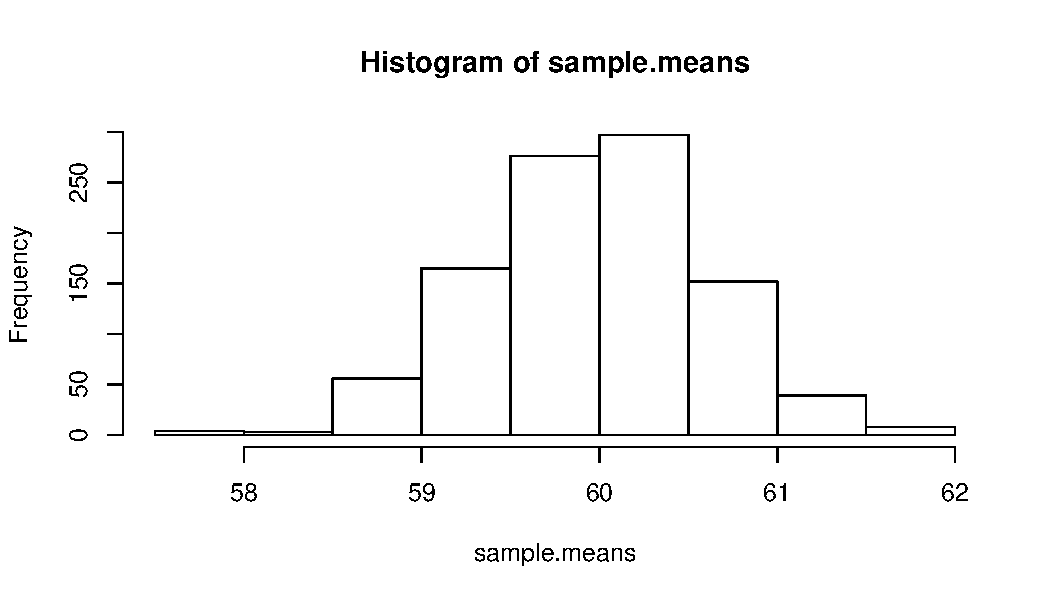
\includegraphics[width=\maxwidth]{figure/unnamed-chunk-16-1} 

\end{knitrout}
  \caption{The sampling distribution of the sample mean with 1000 samples
    of size 40.}
  \label{fig:sdsmplot40}
\end{figure}

Consider now the situation where our sample size is 100. Note that the
mean and standard deviation of the population ages is the same as
above.

\begin{knitrout}
\definecolor{shadecolor}{rgb}{0.969, 0.969, 0.969}\color{fgcolor}\begin{kframe}
\begin{alltt}
\hlstd{sample.means} \hlkwb{<-} \hlkwd{rep}\hlstd{(}\hlnum{NA}\hlstd{,}\hlnum{1000}\hlstd{)}

\hlkwa{for}\hlstd{(i} \hlkwa{in} \hlnum{1}\hlopt{:}\hlnum{1000}\hlstd{)\{}
  \hlstd{sample.100} \hlkwb{<-} \hlkwd{rnorm}\hlstd{(}\hlnum{100}\hlstd{,}\hlkwc{mean}\hlstd{=}\hlnum{60}\hlstd{,}\hlkwc{sd}\hlstd{=}\hlnum{4}\hlstd{)}
  \hlstd{sample.means[i]} \hlkwb{<-} \hlkwd{mean}\hlstd{(sample.100)}
\hlstd{\}}
\end{alltt}
\end{kframe}
\end{knitrout}

\begin{knitrout}
\definecolor{shadecolor}{rgb}{0.969, 0.969, 0.969}\color{fgcolor}\begin{kframe}
\begin{alltt}
\hlstd{means100} \hlkwb{<-} \hlkwd{mean}\hlstd{(sample.means)}
\hlstd{sd100} \hlkwb{<-} \hlkwd{sd}\hlstd{(sample.means)}
\end{alltt}
\end{kframe}
\end{knitrout}


In this particular simulation run, the mean of the means is
60 
and the standard deviation of the
distribution of means is 0.3982. Let's plot
the distribution of the means (Figure~\ref{fig:sdsmplot100}).



\begin{figure}[!htbp]
\centering
\begin{knitrout}
\definecolor{shadecolor}{rgb}{0.969, 0.969, 0.969}\color{fgcolor}
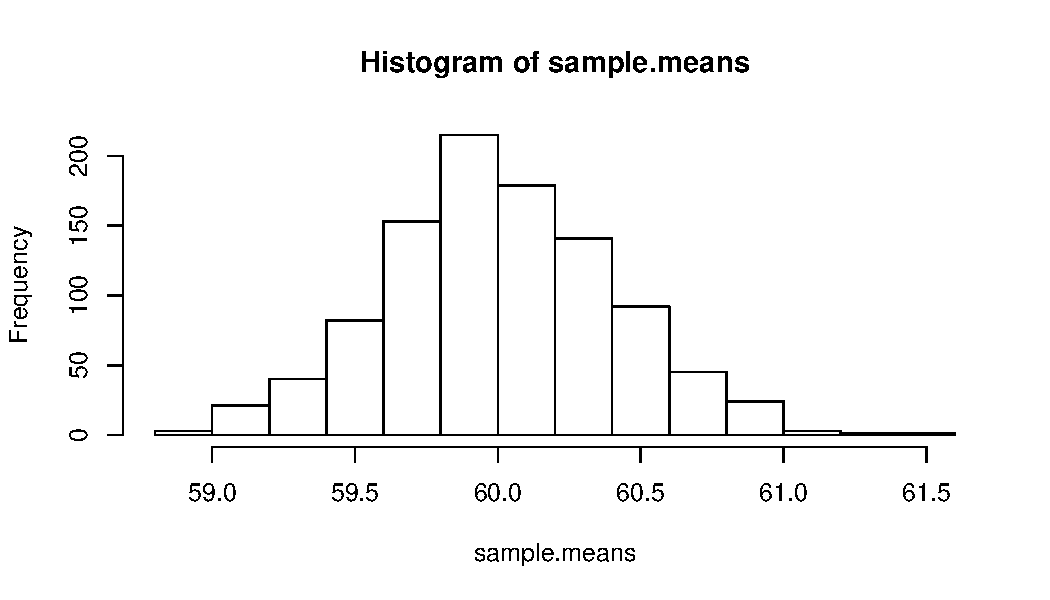
\includegraphics[width=\maxwidth]{figure/unnamed-chunk-19-1} 

\end{knitrout}
\caption{The sampling distribution of the sample mean with samples of size
100.} \label{fig:sdsmplot100}
\end{figure}

The above simulations show us several things. First, the standard
deviation of the distribution of means gets smaller as we increase
sample size.  When the sample size is 40, the standard deviation is
0.6342; when it is 100, the standard deviation
is 0.3982.  Second, as the sample size is
increased, the mean of the sample means 
becomes a better and better estimate of the
\textit{population} mean $\mu_{\bar{x}}$.  A third point (which is not obvious at the
moment) is that there is a lawful relationship between the standard
deviation $\sigma$ of the population and the standard deviation of the
\textit{distribution of means}, which we will call $\sigma_{\bar{x}}$. 
%(Technically, this should be $\sigma_{\bar{X}}$, where $\bar{X}$ is a random variable. I will come to this later.) 
This relationship is:

\begin{equation} \label{sigmabar}
\sigma_{\bar{x}} = \frac{\sigma}{\sqrt{n}}
\end{equation}

\noindent
Here, $n$ is the sample size.  It is possible to derive equation
\ref{sigmabar} from first principles, but for that we need a bit more theory, which won't cover in this course (see \cite{kerns}).
Here, we simply note the important point that $n$ is in the denominator in this equation, so there is an inverse relationship between the sample size and the standard deviation of the sample means.
Let's take this equation on trust for the moment and use it to compute
$\sigma_{\bar{x}}$ by using the population standard deviation (which
we assume we know). Let's do this for a sample of size 40 and another of size
100:

\begin{knitrout}
\definecolor{shadecolor}{rgb}{0.969, 0.969, 0.969}\color{fgcolor}\begin{kframe}
\begin{alltt}
\hlnum{4}\hlopt{/}\hlkwd{sqrt}\hlstd{(}\hlnum{40}\hlstd{)}
\end{alltt}
\begin{verbatim}
## [1] 0.6324555
\end{verbatim}
\begin{alltt}
\hlnum{4}\hlopt{/}\hlkwd{sqrt}\hlstd{(}\hlnum{100}\hlstd{)}
\end{alltt}
\begin{verbatim}
## [1] 0.4
\end{verbatim}
\end{kframe}
\end{knitrout}

\noindent
The above calculation is consistent with what we just saw: $\sigma_{\bar{x}}$ gets smaller and
smaller as we increase sample size.

We have also introduced a notational convention that we will use
throughout the notes: \index{sample statistic}sample statistics are symbolized by Latin letters
($\bar{x}, s$); \index{population parameter}population parameters are symbolized by Greek letters
($\mu, \sigma$).

\section{The \index{Central Limit Theorem}Central Limit Theorem}

We will see now that the \textit{sampling
distribution of the sample mean} is also normally distributed. In the above example the means were
drawn from a population with normally distributed scores.  It
turns out that the sampling distribution of the sample mean will be
normal even if the population is not normally distributed, as long as
the sample size is large enough and the distribution we are sampling from has a mean. This is known as the Central Limit
Theorem:

\begin{quote}
When sampling from a population that has a mean,	
  provided the sample size is large enough, the sampling distribution
  of the sample mean will be close to normal regardless of the shape of the population distribution.
\end{quote}

[Note: Note the caveat ``When sampling from a population that has a mean''. There are some distributions which do not have a mean; but in this course we will ignore these. More advanced textbooks on probability discuss these distributions.]

Let's check whether this theorem holds
by testing it in a case where our population is not normally distributed.
Let's take our samples from
a population (Figure~\ref{fig:exppopulation}) whose values are distributed exponentially with the same
mean of 60 (the mean of an \index{distribution, exponential}\textsc{exponential distribution} is the reciprocal of the so-called `rate' parameter).




\begin{figure}[!htbp]
  \centering
\begin{knitrout}
\definecolor{shadecolor}{rgb}{0.969, 0.969, 0.969}\color{fgcolor}
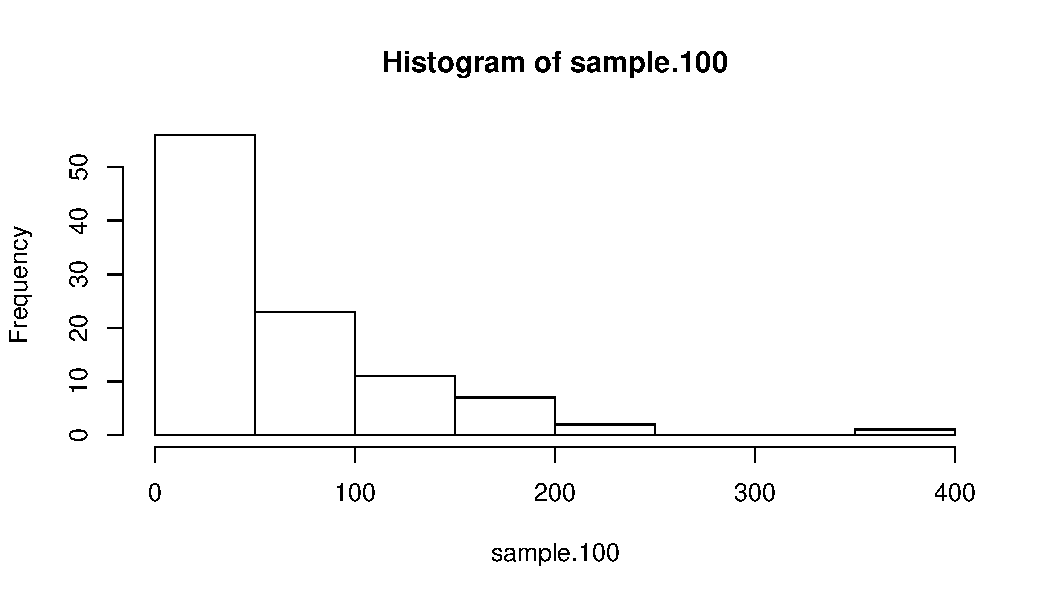
\includegraphics[width=\maxwidth]{figure/unnamed-chunk-21-1} 

\end{knitrout}
  \caption{A sample from exponentially distributed population scores.}
  \label{fig:exppopulation}
\end{figure}

Now let us plot the sampling distribution of the sample mean. We take
1000 samples of size 100 each from this exponentially distributed
population.
As shown in Figure~\ref{fig:exponentialsdsm}, the distribution of the means is again (more or less) normal.



\noindent
Recall that the mean of each sample is a point estimate of the
true mean of the population. Some of these samples will have a mean slightly above
the true mean, some slightly below, and the sampling distribution of
\emph{these} values is roughly normal.  Try altering the sample size
in this example to get a feel for what happens if the sample size is
not `large enough.'

To summarize:

\begin{enumerate}
\item The sampling distribution of the sample mean is normal for large sample sizes. 
\item The mean of the sampling distribution of the sample mean is (in
  the limit) the same as the population mean.
\item It follows from the above two facts that the mean of a sample is
  a good estimate of the population mean.
\end{enumerate}

\begin{figure}[!htbp]
  \centering
\begin{knitrout}
\definecolor{shadecolor}{rgb}{0.969, 0.969, 0.969}\color{fgcolor}
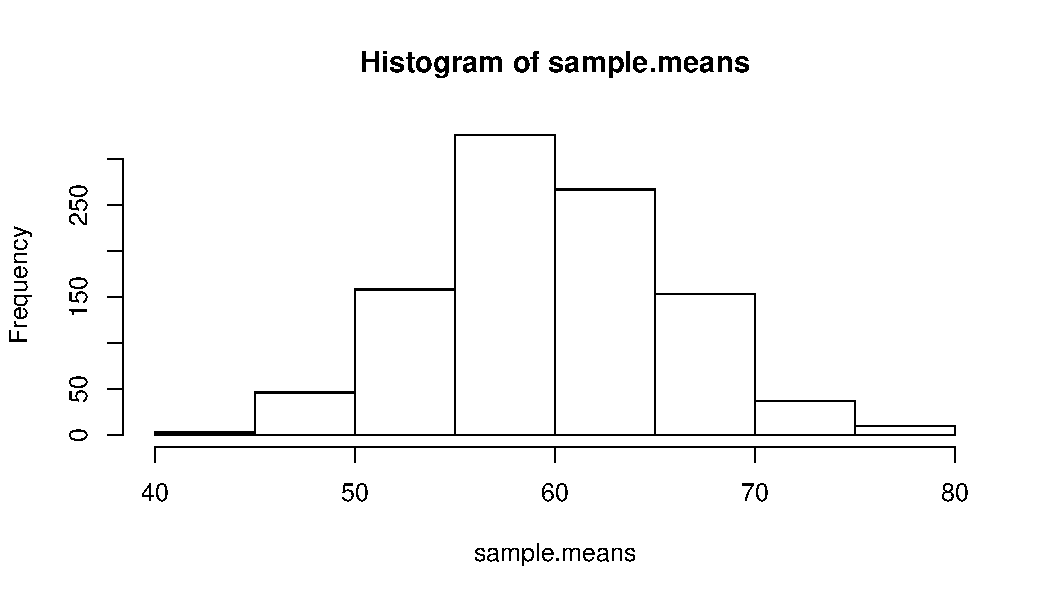
\includegraphics[width=\maxwidth]{figure/unnamed-chunk-22-1} 

\end{knitrout}
  \caption{The sampling distribution of sample mean from an exponentially distributed population.}  \label{fig:exponentialsdsm}
\end{figure}

\section{$\sigma$ and $\sigma_{\bar{x}}$}

We saw earlier that the standard deviation of the sampling
distribution of the sample mean $\sigma_{\bar{x}}$ gets
smaller as we increase sample size. When the sample has size 40, this
standard deviation is 0.6342; when it
is 100, this standard deviation is
0.3982.

Let's study the relationship between $\sigma_{\bar{x}}$ and $\sigma$.
Recall that our population mean $\mu$ = 60, $\sigma$ = 4.  The equation below
summarizes the relationship; it shouldn't surprise you, since we just
saw it above:

\begin{equation}
\sigma_{\bar{x}} = \frac{\sigma}{\sqrt{n}}
\end{equation}

But note also that the ``tighter'' the distribution, the lower the variance about the true population mean.  So the $\sigma_{\bar{x}}$  is an
indicator of how good our estimate of the population mean is.
As we increase the size of a single sample, the smaller the standard
deviation of its corresponding sampling distribution becomes. This brings us to the 95\% confidence interval.

\section {The 95\% Confidence Interval for the Sample Mean}

Let's take a sample of 11 ages from a normally distributed population
with known mean age $\mu = 60$ years and SD $\sigma = 4$ years.

\begin{knitrout}
\definecolor{shadecolor}{rgb}{0.969, 0.969, 0.969}\color{fgcolor}\begin{kframe}
\begin{alltt}
\hlstd{sample.11} \hlkwb{<-} \hlkwd{rnorm}\hlstd{(}\hlnum{11}\hlstd{,}\hlkwc{mean}\hlstd{=}\hlnum{60}\hlstd{,}\hlkwc{sd}\hlstd{=}\hlnum{4}\hlstd{)}
\end{alltt}
\end{kframe}
\end{knitrout}

We know the mean here, but let's pretend we don't.
Let's estimate a population mean from this sample using the sample
mean $\bar{x}$, and compute the SD $\sigma_{\bar{x}}$ of the corresponding sampling distribution. 
Since we know the
true population standard deviation we can get a precise value
for $\sigma_{\bar{x}}$. We don't need to estimate the SD or the $\sigma_{\bar{x}}$.
So, we have an estimate of the true mean, but we know the exact  $\sigma_{\bar{x}}$.


\begin{knitrout}
\definecolor{shadecolor}{rgb}{0.969, 0.969, 0.969}\color{fgcolor}\begin{kframe}
\begin{alltt}
\hlstd{estimated.mean} \hlkwb{<-} \hlkwd{mean}\hlstd{(sample.11)}
\hlstd{SD.population} \hlkwb{<-} \hlnum{4}
\hlstd{n} \hlkwb{<-} \hlkwd{length}\hlstd{(sample.11)}
\hlstd{SD.distribution} \hlkwb{<-} \hlstd{SD.population}\hlopt{/}\hlkwd{sqrt}\hlstd{(n)}
\end{alltt}
\end{kframe}
\end{knitrout}

We know from the Central Limit Theorem that the sampling distribution
of the sample mean is roughly normal, and we know that in this case 
$\sigma_{\bar{x}} =$ 1.2.  
Note that if we repeatedly sample from this population, our sample mean will change slightly each time, but the $\sigma_{\bar{x}}$ is not going to change. Why is that?


It turns out that the probability that the population mean is within $2\times 
\sigma_{\bar{x}}$ of the sample mean is a bit over $0.95$. Let's
calculate this range, $2\times 
\sigma_{\bar{x}}$:

\begin{align}
\bar{x} \pm (2 \times \sigma_{\bar{x}}) & = \hbox{62} \pm (2 \times \hbox{1.206}) 
\end{align}

The 0.95 probability region is between
59.4 and
64.2.  The probability region we compute is centered around the \textbf{estimated} mean. If we repeatedly sample from this population, we will get different sample means each time, but the width of the interval would remain identical if we use the exact $\sigma_{\bar{x}}$ value we computed above. That means that under repeated sampling, the location of the mean and therefore the location of the probability region will vary. 

The key thing to understand here is that probability region is centered around the \textbf{sample} mean, which will vary with each sample even if we sample from a population with a given distribution with a specific mean and standard deviation.

%The probability region is called the 95\% \index{confidence interval}confidence interval (CI).

Suppose now that sample size was four times bigger (44). Let's again
calculate the sample mean, the standard deviation of the corresponding 
sampling distribution, and from this information,
compute the 95\% confidence interval. First, we need to compute $\sigma_{\bar{x}}$:

\begin{knitrout}
\definecolor{shadecolor}{rgb}{0.969, 0.969, 0.969}\color{fgcolor}\begin{kframe}
\begin{alltt}
\hlstd{sample.44} \hlkwb{<-} \hlkwd{rnorm}\hlstd{(}\hlnum{44}\hlstd{,}\hlkwc{mean}\hlstd{=}\hlnum{60}\hlstd{,}\hlkwc{sd}\hlstd{=}\hlnum{4}\hlstd{)}
\hlstd{estimated.mean} \hlkwb{<-} \hlkwd{mean}\hlstd{(sample.44)}
\hlstd{n} \hlkwb{<-} \hlkwd{length}\hlstd{(sample.44)}
\hlstd{(SD.distribution} \hlkwb{<-} \hlstd{SD.population}\hlopt{/}\hlkwd{sqrt}\hlstd{(n))}
\end{alltt}
\begin{verbatim}
## [1] 0.6030227
\end{verbatim}
\end{kframe}
\end{knitrout}

Now we get a much tighter 95\% confidence interval:

\begin{align}
\bar{x} \pm 2 \times \sigma_{\bar{x}} & = \hbox{60} \pm 2 \times \hbox{0.603} 
\end{align}

The interval now is between 58.5
and 60.9, smaller
than the one we got for the smaller sample size.
In fact, it is exactly half as wide. Take a moment to make sure you understand why.

\section{Realistic Statistical Inference}

Until now we have been sampling from a population whose mean and
standard deviation we know. However, we normally don't know the
population parameters. In other words, although we know that:

\begin{equation}
\sigma_{\bar{x}} = \frac{\sigma}{\sqrt{n}}
\end{equation}

\noindent
when we take samples in real life, we usually don't know $\sigma$. 
After all, it is based on an average of squared distances from the population mean $\mu$, and that is usually the very thing we are trying to estimate!

What we \emph{do} have, however, is the standard deviation \emph{of the sample itself} (denoted $s$). This in turn means that we can only get an \textit{estimate} of
$\sigma_{\bar{x}}$.  
This is called the \index{standard error}\textsc{standard error} (SE) or estimated standard error of the 
  sample mean:
\begin{equation}
SE_{\bar{x}} = \frac{s}{\sqrt{n}}
\end{equation}

Pay careful attention to the distinction between $s$ (an estimate of the standard deviation of the population
$\sigma$) and $SE_{\bar{x}}$ (an estimate of the standard deviation of the sampling distribution, which is in turn based on $s$).  

We saw previously that the size of $\sigma_{\bar{x}}$---a measure of the spread of the sampling distribution---is crucial in determining the size of a 95\% confidence interval for a particular sample. Now we only have an estimate of that spread. Moreover, the estimate will change from sample to sample, as the value of $s$ changes. This introduces a new level of uncertainty into our task: the quantity $\sigma_{\bar{x}}$ has become an estimate based on an estimate! Intuitively, we would expect the confidence interval to increase in size, reflecting this increase in uncertainty. We will see how to quantify this intuition presently.

First, however, we should explore the pattern of variability in this new statistic we have introduced, $s$, which (like the sample mean) will vary randomly from sample to sample. Can we safely assume
that $s$ is a reliable estimate of $\sigma$? 

\section{$s^2$ provides a good estimate of $\sigma^2$}

Earlier in this chapter we repeatedly sampled from a population of
people with mean age 60 years and standard deviation 4 years; then we plotted the
distribution of sample means that resulted from the repeated samples.
One thing we noticed was that the sample means tended to be clustered around the value corresponding to the population mean (60).
Let's repeat this experiment, but this time we plot the distribution
of the samples' variances 
(Figure~\ref{fig:varsample}). 





\begin{figure}[!htbp]
  \centering
\begin{knitrout}
\definecolor{shadecolor}{rgb}{0.969, 0.969, 0.969}\color{fgcolor}
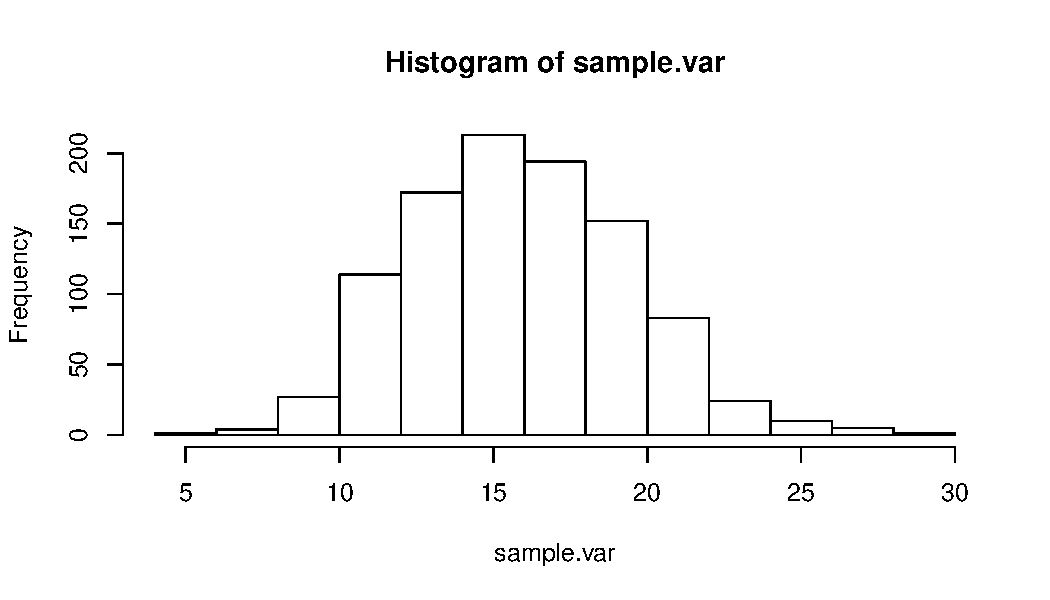
\includegraphics[width=\maxwidth]{figure/unnamed-chunk-26-1} 

\end{knitrout}
  \caption{The distribution of the sample variance,
    sample size 40.}
  \label{fig:varsample}
\end{figure}

Figure~\ref{fig:varsample} shows that the sample variances $s^2$ tend to cluster around the population variance (16). 
%This is related to the fact that $s^2$ is an \index{unbiased estimator}\textsc{unbiased estimator} of $\sigma^2$. 
This is true even if  we have an exponentially distributed population whose variance is 1 (Figure~\ref{fig:varsampleexp}).



\begin{figure}[!htbp]
  \centering
\begin{knitrout}
\definecolor{shadecolor}{rgb}{0.969, 0.969, 0.969}\color{fgcolor}
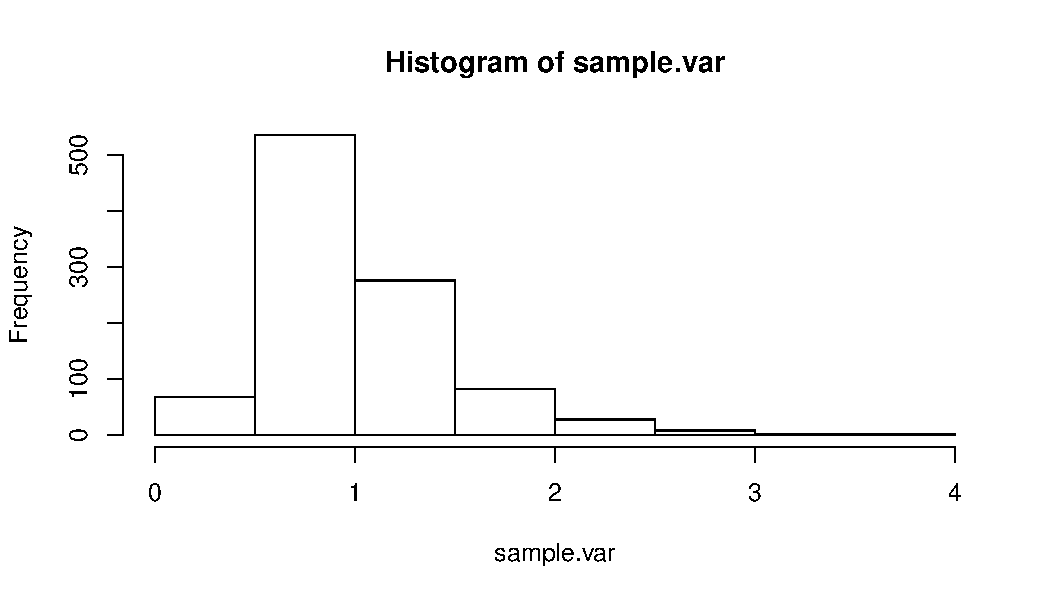
\includegraphics[width=\maxwidth]{figure/unnamed-chunk-27-1} 

\end{knitrout}
  \caption{The sampling distribution of sample variances from an exponentially distributed population.}
  \label{fig:varsampleexp}
\end{figure}

%Now, although $s^2$ is a good estimate of $\sigma^2$, $s$ is not a very good estimator of $\sigma$ (see \cite{lehmann1998theory}). Nevertheless,
We use the square root of the sample variance  $s$ as an estimate of the unknown population standard
deviation $\sigma$. This in turn allows us to estimate the standard deviation of the sampling distribution $\sigma_{\bar{x}}$ using the Standard Error $SE_{\bar{x}}$.

Notice that the Standard Error will vary from sample to sample, since the estimate $s$ of the population parameter $\sigma$ will vary from sample to sample. And of course, as the sample size increases the estimate $s$ becomes more accurate, as does the SE, suggesting that the uncertainty introduced by this extra layer of estimation will be more of an issue for smaller sample sizes.

Our problem now is that 
the sampling distribution of the sample mean will take the estimate $s$ from the sample, not $\sigma$, as a parameter.
If we were to derive some value $v$ for the SE, and simply plug this in to the normal distribution for the sample statistic, this would be equivalent to claiming that $v$ \emph{really was} the population parameter $\sigma$.

What we require is a distribution whose shape has greater uncertainty built into it than
the normal distribution. This is the motivation for using the so-called
t-\textsc{distribution}, which we turn to next.

\section{The \index{t-distribution}t-distribution}

As discussed above, the distribution we use with an estimated $s$ needs to reflect greater uncertainty at small sample sizes. There is in fact a family of t-distribution curves whose shapes vary with sample size. In the limit, if the sample size were infinity, the t-distribution would be indistinguishable from the normal distribution. The t-curve becomes more like the normal distribution in shape as sample size increases.
This t-distribution is formally defined by the \textsc{degrees of freedom} (which is simply sample size
minus 1 in this case; we won't worry too much about what degrees of freedom means at this stage) and, for small sample sizes, it has more of the total probability located in
the tails of the distribution. It follows that the probability of a sample mean being close to the true mean is slightly lower when measured by this distribution, reflecting our
greater uncertainty. You can see this effect in Figure~\ref{fig:tversusnorm} at small sample sizes. But notice
that with about 15 degrees of freedom, the t-distribution is
already very close to normal.




\begin{figure}[!htbp]
  \centering
\begin{knitrout}
\definecolor{shadecolor}{rgb}{0.969, 0.969, 0.969}\color{fgcolor}
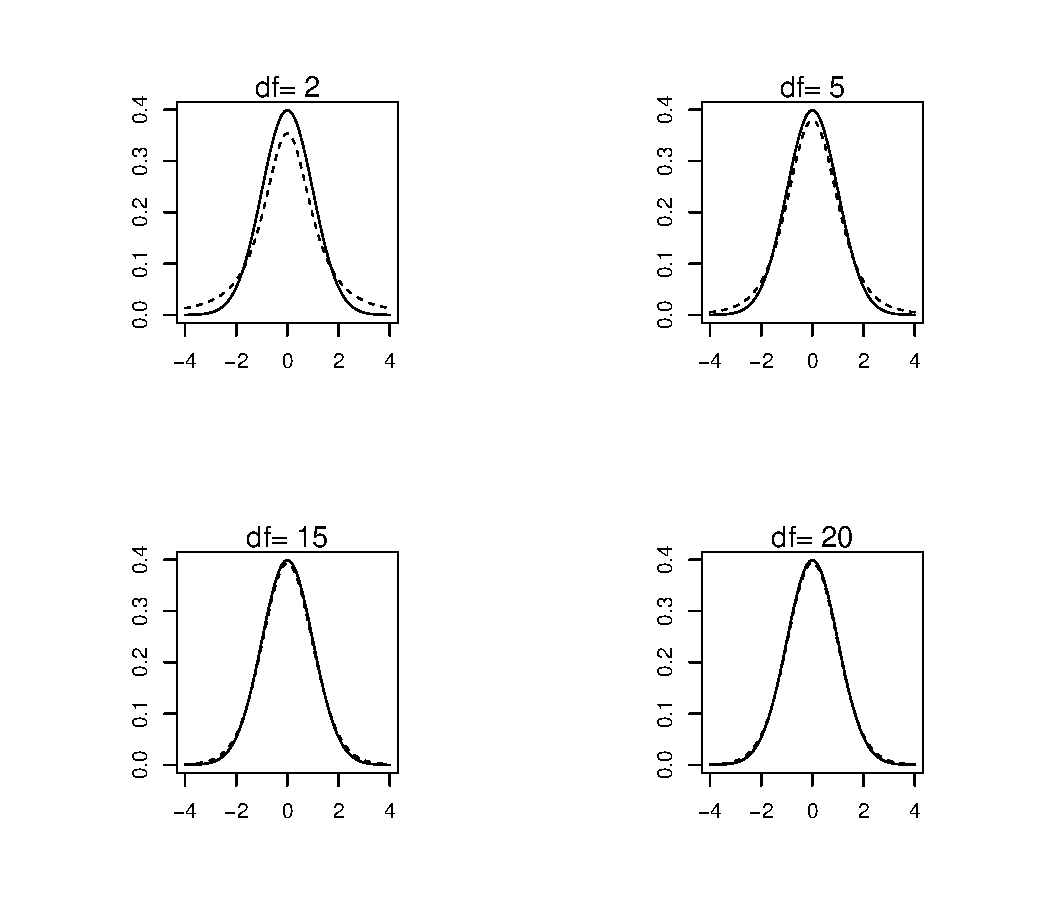
\includegraphics[width=\maxwidth]{figure/unnamed-chunk-28-1} 

\end{knitrout}
  
  \caption{A comparison between the normal (solid line) and t-distribution (broken line) for different degrees of freedom.}
  \label{fig:tversusnorm}
\end{figure}


The formal definition of the t-distribution is as follows:
Suppose we have a random sample of size $n$, say of reading times (RTs), and these RTs come from a $N(\mathtt{mean}=\mu,\,\mathtt{sd}=\sigma)$ distribution. Then the quantity 

\begin{equation}
T=\frac{\overline{X}-\mu}{S/\sqrt{n}}
\end{equation}

has a $\mathsf{t}(\mathtt{df}=n-1)$ sampling distribution. The distribution is defined as ($r$ is degrees of freedom; see below):

\begin{equation}
f_{X}(x,r)=\frac{\Gamma[(r+1)/2]}{\sqrt{r\pi}\ \Gamma(r/2)}\left(1+\frac{x^{2}}{r}\right)^{-(r+1)/2},\quad -\infty < x < \infty.
\end{equation}

[$\Gamma$ refers to the gamma function; in this course we can ignore what this is, but read \cite{kerns} if you are interested.]

The $t$ distribution is defined by its $r=n-1$ degrees of freedom, and we will write that the sample scores are coming from $\mathsf{t}(\mathtt{df}=r)$. The shape of the function for the t distribution is similar to the normal, but the tails are considerably heavier for small sample sizes.  As with the normal distribution, there are four functions in $\mathsf{R}$ associated with the $t$ distribution, namely \texttt{dt}, \texttt{pt}, \texttt{qt}, and \texttt{rt}, which behave like \texttt{dnorm}, \texttt{pnorm}, \texttt{qnorm}, and \texttt{rnorm}.


What do we have available to us to work with now? We have an estimate
$s$ of the population SD, and so an estimate $SE_{\bar{x}}$ of the SD
of the sampling distribution:
\begin{equation}
SE_{\bar{x}} = \frac{s}{\sqrt{n}}
\end{equation}

We also have a more spread-out distribution than the normal (at least for smaller sample sizes), the
t-distribution, defined by the degrees of freedom (sample size minus 1).  We are
now ready to do realistic statistical inference.


\section{The \index{t-test}One-sample t-test}

%How do we build a confidence interval based on this new model of inference?

We start by taking a random sample of
11 peoples' ages from a population with mean age 60 years and standard deviation 4 years.

\begin{knitrout}
\definecolor{shadecolor}{rgb}{0.969, 0.969, 0.969}\color{fgcolor}\begin{kframe}
\begin{alltt}
\hlstd{sample} \hlkwb{<-} \hlkwd{rnorm}\hlstd{(}\hlnum{11}\hlstd{,}\hlkwc{mean}\hlstd{=}\hlnum{60}\hlstd{,}\hlkwc{sd}\hlstd{=}\hlnum{4}\hlstd{)}
\end{alltt}
\end{kframe}
\end{knitrout}

\noindent
%Using this sample, we can compute something very useful called a ``t-value'' by using a built-in t-test function:

%We could have done this ``by hand'':

%We'll just get back to what this t-value tells us.
We can  
ask for the  95\% confidence interval, which (we saw this earlier) is \textit{roughly} two times the Standard Error:

\begin{knitrout}
\definecolor{shadecolor}{rgb}{0.969, 0.969, 0.969}\color{fgcolor}\begin{kframe}
\begin{alltt}
\hlkwd{t.test}\hlstd{(sample)}\hlopt{$}\hlstd{conf.int}
\end{alltt}
\begin{verbatim}
## [1] 59.26122 63.11509
## attr(,"conf.level")
## [1] 0.95
\end{verbatim}
\end{kframe}
\end{knitrout}



Note that all of the information required to calculate this t-value is contained in the sample itself: the sample mean; the sample size and sample standard deviation $s$ (from which we compute the SE), the degrees of freedom (the sample size minus 1, from which we reference the appropriate t-distribution).
Sure enough, if our sample size had been larger, our CI would be narrower:

\begin{knitrout}
\definecolor{shadecolor}{rgb}{0.969, 0.969, 0.969}\color{fgcolor}\begin{kframe}
\begin{alltt}
\hlstd{sample} \hlkwb{<-} \hlkwd{rnorm}\hlstd{(}\hlnum{100}\hlstd{,}\hlkwc{mean}\hlstd{=}\hlnum{60}\hlstd{,}\hlkwc{sd}\hlstd{=}\hlnum{4}\hlstd{)}
\end{alltt}
\end{kframe}
\end{knitrout}

\begin{knitrout}
\definecolor{shadecolor}{rgb}{0.969, 0.969, 0.969}\color{fgcolor}\begin{kframe}
\begin{alltt}
\hlkwd{t.test}\hlstd{(sample)}\hlopt{$}\hlstd{conf.int}
\end{alltt}
\begin{verbatim}
## [1] 59.82366 61.43996
## attr(,"conf.level")
## [1] 0.95
\end{verbatim}
\end{kframe}
\end{knitrout}

%What about the t-value? Is it likely to be smaller if we increase sample size?

Given the specific sample values you get by running the above command that results in the object \texttt{sample}, try to reproduce this confidence interval by hand.  Do this after the lecture for this chapter has been presented.


\section{Some Observations on Confidence Intervals} \label{confidenceintervals}

\label{trickypoint}
\index{confidence interval}
There are some subtleties associated with confidence intervals that
are often not brought up in elementary discussions, simply because the
issues are just too daunting to tackle. However, we will use
simulations to unpack some of these subtleties. The issues are in reality quite simple.

The first critical point to understand is the meaning of the
confidence interval. 
Is the 95\%
confidence interval telling you the range within which we are 95\% sure
that the population mean lies? No!

Notice
is that the range defined by the confidence interval will vary with
each sample even if the sample size is kept constant. The reason is
that the sample mean will vary each time, and the standard deviation will
vary too. We can check this fact quite easily.

First we define a function for computing 95\% CIs:\footnote{Here, we use the built-in R function called \texttt{qt(p,DF)} which, for a given confidence-interval range (say, 0.975), and a given degrees of freedom, DF, tells you the corresponding critical t-value.}

\begin{knitrout}
\definecolor{shadecolor}{rgb}{0.969, 0.969, 0.969}\color{fgcolor}\begin{kframe}
\begin{alltt}
\hlstd{se} \hlkwb{<-} \hlkwa{function}\hlstd{(}\hlkwc{x}\hlstd{)}
      \hlstd{\{}
        \hlstd{y} \hlkwb{<-} \hlstd{x[}\hlopt{!}\hlkwd{is.na}\hlstd{(x)]} \hlcom{# remove the missing values, if any}
        \hlkwd{sqrt}\hlstd{(}\hlkwd{var}\hlstd{(}\hlkwd{as.vector}\hlstd{(y))}\hlopt{/}\hlkwd{length}\hlstd{(y))}
\hlstd{\}}


\hlstd{ci} \hlkwb{<-} \hlkwa{function} \hlstd{(}\hlkwc{scores}\hlstd{)\{}
\hlstd{m} \hlkwb{<-} \hlkwd{mean}\hlstd{(scores,}\hlkwc{na.rm}\hlstd{=}\hlnum{TRUE}\hlstd{)}
\hlstd{stderr} \hlkwb{<-} \hlkwd{se}\hlstd{(scores)}
\hlstd{len} \hlkwb{<-} \hlkwd{length}\hlstd{(scores)}
\hlstd{upper} \hlkwb{<-} \hlstd{m} \hlopt{+} \hlkwd{qt}\hlstd{(}\hlnum{.975}\hlstd{,} \hlkwc{df}\hlstd{=len}\hlopt{-}\hlnum{1}\hlstd{)} \hlopt{*} \hlstd{stderr}
\hlstd{lower} \hlkwb{<-} \hlstd{m} \hlopt{+} \hlkwd{qt}\hlstd{(}\hlnum{.025}\hlstd{,} \hlkwc{df}\hlstd{=len}\hlopt{-}\hlnum{1}\hlstd{)} \hlopt{*} \hlstd{stderr}
\hlkwd{return}\hlstd{(}\hlkwd{data.frame}\hlstd{(}\hlkwc{lower}\hlstd{=lower,}\hlkwc{upper}\hlstd{=upper))}
\hlstd{\}}
\end{alltt}
\end{kframe}
\end{knitrout}

\noindent

Next, we take 100 samples repeatedly from a population with mean 60 and SD 4, computing the 95\% CI each time.

\begin{knitrout}
\definecolor{shadecolor}{rgb}{0.969, 0.969, 0.969}\color{fgcolor}\begin{kframe}
\begin{alltt}
\hlstd{lower} \hlkwb{<-} \hlkwd{rep}\hlstd{(}\hlnum{NA}\hlstd{,}\hlnum{100}\hlstd{)}
\hlstd{upper} \hlkwb{<-} \hlkwd{rep}\hlstd{(}\hlnum{NA}\hlstd{,}\hlnum{100}\hlstd{)}

\hlkwa{for}\hlstd{(i} \hlkwa{in} \hlnum{1}\hlopt{:}\hlnum{100}\hlstd{)\{}
  \hlstd{sample} \hlkwb{<-} \hlkwd{rnorm}\hlstd{(}\hlnum{100}\hlstd{,}\hlkwc{mean}\hlstd{=}\hlnum{60}\hlstd{,}\hlkwc{sd}\hlstd{=}\hlnum{4}\hlstd{)}
  \hlstd{lower[i]} \hlkwb{<-} \hlkwd{ci}\hlstd{(sample)}\hlopt{$}\hlstd{lower}
  \hlstd{upper[i]} \hlkwb{<-} \hlkwd{ci}\hlstd{(sample)}\hlopt{$}\hlstd{upper}
\hlstd{\}}

\hlstd{cis} \hlkwb{<-} \hlkwd{cbind}\hlstd{(lower,upper)}

\hlkwd{head}\hlstd{(cis)}
\end{alltt}
\begin{verbatim}
##         lower    upper
## [1,] 59.04479 60.67648
## [2,] 59.14636 60.83086
## [3,] 59.41300 60.86026
## [4,] 59.69198 61.31214
## [5,] 59.38109 61.23145
## [6,] 58.75346 60.54439
\end{verbatim}
\end{kframe}
\end{knitrout}


Thus, the center and the size of any one confidence interval, based on a single
sample, will depend on the
particular sample mean and standard deviation you happen to observe for
that sample.  The sample mean and standard deviation 
are good estimates the population mean and standard
deviation, but they are ultimately just estimates of these true
parameters.

Importantly, because of the shapes of the distribution of
sample means and the variances, if we
repeatedly sample from a population and compute the confidence
intervals each time, approximately 95\% \textbf{of the confidence
intervals} will contain the population mean. In
the other 5\% or so of the cases, the confidence intervals
will not contain the population mean. 

This is what `the' 95\% confidence
interval means: it's a statement about confidence intervals computed with hypothetical repeated samples. Hypothetical means you haven't actually carried out that repeated sampling.
 More specifically, it's a statement about the probability that the hypothetical confidence intervals (that would be computed
from the hypothetical repeated samples, had you did that repeated sampling) will contain the population mean. It is incorrect to to make any probability statement about the single CI you compute from a single sample.

So let's check the above statement about the meaning of the CI. We can repeatedly sample, and repeatedly build 95\% CIs, and
determine whether the population mean lies within them. The claim is
that the population mean will be in 95\% of the CIs.

\begin{knitrout}
\definecolor{shadecolor}{rgb}{0.969, 0.969, 0.969}\color{fgcolor}\begin{kframe}
\begin{alltt}
\hlstd{store} \hlkwb{<-} \hlkwd{rep}\hlstd{(}\hlnum{NA}\hlstd{,}\hlnum{100}\hlstd{)}

\hlstd{pop.mean}\hlkwb{<-}\hlnum{60}
\hlstd{pop.sd}\hlkwb{<-}\hlnum{4}

\hlkwa{for}\hlstd{(i} \hlkwa{in} \hlnum{1}\hlopt{:}\hlnum{100}\hlstd{)\{}
  \hlstd{sample} \hlkwb{<-} \hlkwd{rnorm}\hlstd{(}\hlnum{100}\hlstd{,}\hlkwc{mean}\hlstd{=pop.mean,}\hlkwc{sd}\hlstd{=pop.sd)}
  \hlstd{lower[i]} \hlkwb{<-} \hlkwd{ci}\hlstd{(sample)}\hlopt{$}\hlstd{lower}
  \hlstd{upper[i]} \hlkwb{<-} \hlkwd{ci}\hlstd{(sample)}\hlopt{$}\hlstd{upper}
  \hlkwa{if}\hlstd{(lower[i]}\hlopt{<}\hlstd{pop.mean} \hlopt{&} \hlstd{upper[i]}\hlopt{>}\hlstd{pop.mean)\{}
    \hlstd{store[i]} \hlkwb{<-} \hlnum{TRUE}\hlstd{\}} \hlkwa{else} \hlstd{\{}
      \hlstd{store[i]} \hlkwb{<-} \hlnum{FALSE}\hlstd{\}}
\hlstd{\}}

\hlcom{## need this for the plot below:}
\hlstd{cis} \hlkwb{<-} \hlkwd{cbind}\hlstd{(lower,upper)}


\hlcom{## convert store to factor:}
\hlstd{store}\hlkwb{<-}\hlkwd{factor}\hlstd{(store)}

\hlkwd{summary}\hlstd{(store)}
\end{alltt}
\begin{verbatim}
## FALSE  TRUE 
##     8    92
\end{verbatim}
\end{kframe}
\end{knitrout}


So that's more or less true. 
To drive home the point, we can also plot the confidence intervals to visualize the proportion of cases where each CI contains the population mean (Figure~\ref{repeatedCIsplot}). 



In this figure, we control the width of the lines marking the CI using the information we extracted above (in the object \texttt{store}) to determine whether the population mean is contained in the CI or not: when a CI does not contain the population mean, the line is thicker than when it does contain the mean.
You should try repeatedly sampling from the population as we did above, computing the lower and upper ranges of the 95\% confidence interval, and then plotting the results as shown in Figure~\ref{repeatedCIsplot}.


\begin{figure}
\begin{knitrout}
\definecolor{shadecolor}{rgb}{0.969, 0.969, 0.969}\color{fgcolor}
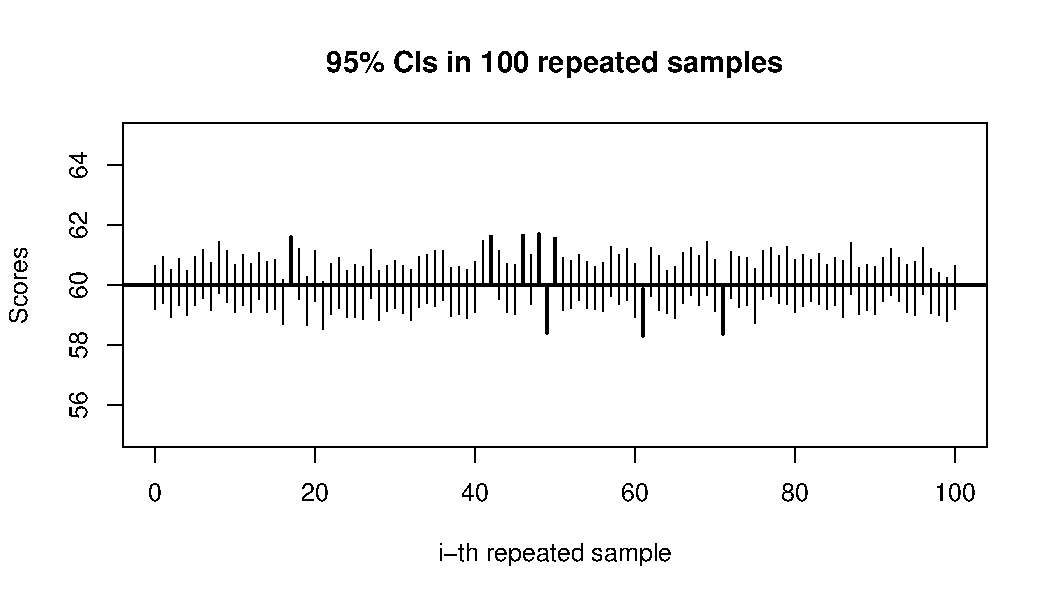
\includegraphics[width=\maxwidth]{figure/unnamed-chunk-36-1} 

\end{knitrout}
\caption{A visualization of the proportion of cases where the
  population mean is contained in the 95\% CI, computed from repeated samples. The CIs that do not contain the population mean are marked with thicker lines.}\label{repeatedCIsplot}
\end{figure}


Note that when we compute a 95\% confidence interval for a particular
sample, we have only \emph{one} interval. 
That \textit{particular} interval does
\emph{not} have the interpretation that the probability that the population mean lies
\emph{within that interval} is $0.95$. 

Thus, the meaning of the confidence interval
depends crucially on hypothetical repeated samples: 95\% of the confidence
intervals in these repeated samples will contain the
population mean. In essence, the confidence interval from a single
sample is in the set $S$ of a random variable, just like heads and tails in a coin toss are in the set $S$ of a random variable. Just as a
fair coin has a 0.5 chance of yielding a heads, a confidence interval has a 0.95 chance of containing the population mean.

The meaning of confidence intervals is confusing enough,
but often (e.g., \cite{mooreetal}), statisticians confuse the issue even further by writing, for a single sample: ``We are 95\% confident that the population mean lies within this [a particular sample's] 95\% CI.'' Here, they are using the word `confidence' with a very specific meaning. Normally, when I say that I am 100\% confident that it will rain today, I mean that the probability of it raining today is 100\%. The above statement, ``We are 95\% confident that the population mean lies within \underline{this} [a particular sample's] 95\% CI.'', uses `confidence' differently; it even uses the word ``this'' in a very misleading way.
Statistics textbooks do not mean that the probability of the population mean being in \underline{that} \underline{one} \underline{specific} confidence interval is 95\%, but rather that ``95\% of the confidence intervals will contain the population mean''. Why this misleading wording? Either they were not paying attention to what they were writing, or they found it cumbersome to say the whole thing each time, so they (statisticians) came up with a short-cut formulation that is incorrect.  Read \cite{hoekstra2014robust} on more discussion about misinterpretations of confidence intervals.

\section{Sample SD and \index{degrees of freedom}Degrees of Freedom} \label{ch3nminusone}

Let's revisit the question: Why do we use $n-1$ in the
equation for standard deviation?  
Recall that the sample standard deviation $s$ is just the square root of the variance:
the average distance of the numbers in the list from the mean of the
numbers:
\begin{equation} 
s^2 = \frac{1}{n-1} \underset{i=1}{\overset{n}{\sum}}(x_i - \bar{x})^2  \label{nminusone}
\end{equation}

We can explore the reason why we use $n-1$ in the context of
estimation by considering what would happen 
if we simply used $n$ instead. As we will see, if we use $n$, then $s^2$
(which is an estimate of the population variance $\sigma^2$) would be
smaller than the true population variance. This smaller $s^2$ turns out to provide a poorer estimate than
when we use $n-1$. Let's verify this using simulations.

We define new variance functions that use $n$, and simulate the sampling distribution of this new statistic from a population with known variance $\sigma^2=1$).
\begin{knitrout}
\definecolor{shadecolor}{rgb}{0.969, 0.969, 0.969}\color{fgcolor}\begin{kframe}
\begin{alltt}
\hlcom{# re-define variance to see whether it underestimates:}
\hlstd{new.var} \hlkwb{<-} \hlkwa{function}\hlstd{(}\hlkwc{x}\hlstd{)\{}
        \hlkwd{sum}\hlstd{((x}\hlopt{-}\hlkwd{mean}\hlstd{(x))}\hlopt{^}\hlnum{2}\hlstd{)} \hlopt{/} \hlkwd{length}\hlstd{(x)}
\hlstd{\}}

\hlstd{correct} \hlkwb{<-} \hlkwd{rep}\hlstd{(}\hlnum{NA}\hlstd{,}\hlnum{1000}\hlstd{)}
\hlstd{incorrect} \hlkwb{<-} \hlkwd{rep}\hlstd{(}\hlnum{NA}\hlstd{,}\hlnum{1000}\hlstd{)}

\hlkwa{for}\hlstd{(i} \hlkwa{in} \hlnum{1}\hlopt{:}\hlnum{1000}\hlstd{)\{}
  \hlstd{sample.10} \hlkwb{<-} \hlkwd{rnorm}\hlstd{(}\hlnum{10}\hlstd{,} \hlkwc{mean}\hlstd{=}\hlnum{0}\hlstd{,} \hlkwc{sd}\hlstd{=}\hlnum{1}\hlstd{)}
  \hlstd{correct[i]} \hlkwb{<-} \hlkwd{var}\hlstd{(sample.10)}
  \hlstd{incorrect[i]} \hlkwb{<-} \hlkwd{new.var}\hlstd{(sample.10)}
\hlstd{\}}
\end{alltt}
\end{kframe}
\end{knitrout}

As shown in Figure~\ref{fig:nminus1}, 
using $n$ gives, on average, an underestimated value of the true
variance. Try this simulation with very large n to see if dividing by n or n-1 makes any difference.




\begin{figure}[!htbp]
  \centering
\begin{knitrout}
\definecolor{shadecolor}{rgb}{0.969, 0.969, 0.969}\color{fgcolor}
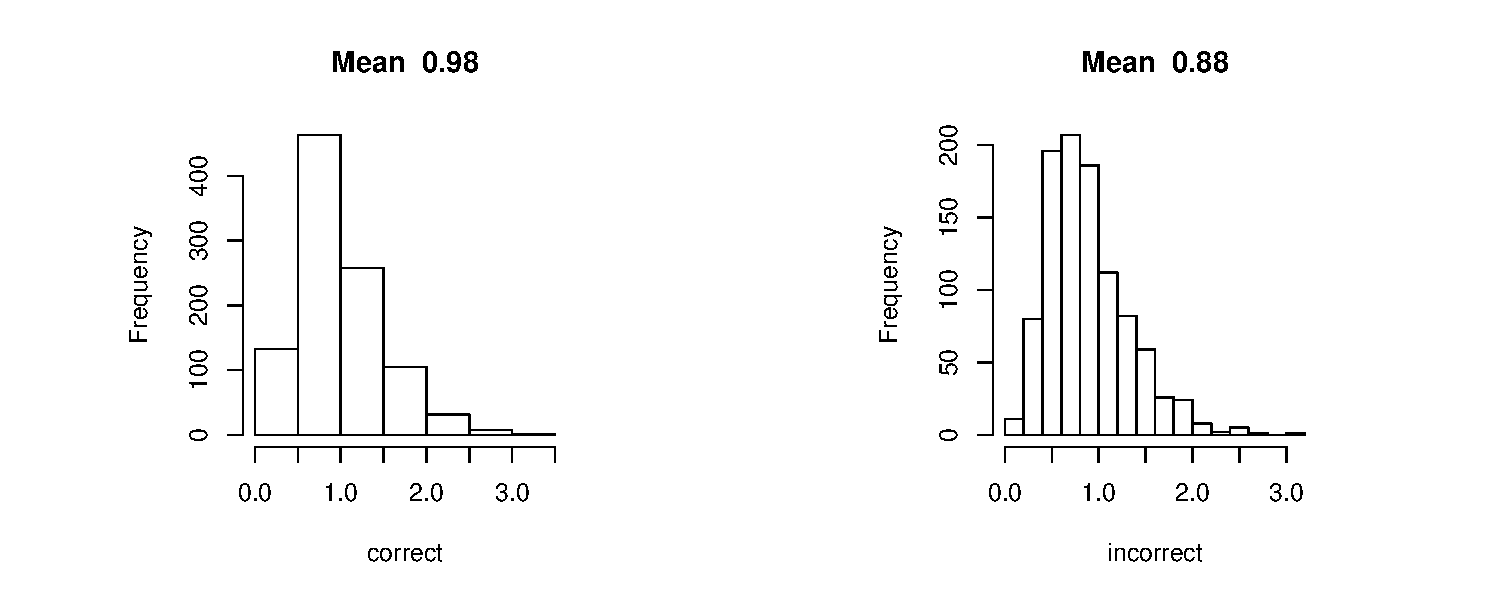
\includegraphics[width=\maxwidth]{figure/unnamed-chunk-38-1} 

\end{knitrout}
\caption{The consequence of taking $n-1$ versus $n$ in the
denominator for calculating variance, sample size 10.}
\label{fig:nminus1}
\end{figure}

As we mentioned earlier, for large $n$ it will not matter much whether we take $n$ or $n-1$. Try it out yourself for large $n$ to see if this is true. For more formal details on the $n$ vs $n-1$ issue, read the book by \cite{kerns}.

\section{Summary of the Sampling Process}

It is useful at this point to summarize the terminology we have been
using, and the logic of sampling. First, take a look at the concepts
we have covered so far. 

We provide a list of the different concepts in
Table~\ref{summaryofnotation} below for easy reference.
Here, $\sigma_{\bar{x}} = \frac{\sigma}{\sqrt{n}}$ and $SE_{\bar{x}} = \frac{s}{\sqrt{n}}$.

\begin{table}[!htbp]
\begin{center}
\caption{A summary of the notation used.}\label{summaryofnotation}
\begin{tabular}{r|r}
The sample statistic~~ & ~~is an estimate of \\
\hline
sample mean $\bar{x}$~~               & population mean $\mu$   \\
sample SD $s$~~                       & population SD $\sigma$ \\
standard error $SE_{\bar{x}}$~~ & sampling distribution $\sigma_{\bar{x}}$ \\ 
\end{tabular}
\end{center}
\end{table}



\begin{enumerate}
\item
Statistical inference usually involves a single sample; due to the central limit theorem, we know that
for large sample sizes, the sampling distribution of the sample mean is normal. \textbf{Important}: this does not mean that you can assume that the distribution of the data, i.e., the individual data points $x_1,\dots, x_n$ that we use to calculate the mean $\bar{x}= \sum_i x_i/n$, is normal. The distribution of the $x_i$ can be LogNormal, Gamma, Exponential, etc. It is a common mistake to think that because the central limit theorem holds for the sampling distribution of the mean, we can now assume that $x_i$ are normally distributed.
\item
The statistic (e.g., sample mean) in a random sample is a good estimate of the population parameter (the population mean).  \textbf{Important}: This is only true in general when sample sizes are large---we return to this point in the next chapter.
\item
The standard
deviation of the sampling distribution of the sample means, $\sigma_{\bar{x}}$, is 
determined by two things: the inherent variability $\sigma$ in the population, and the sample size. 
It tells us how ``tight'' the sampling distribution is.
If $\sigma_{\bar{x}}$ is small, then the distribution has a narrow shape: random samples are more likely to have means very close to
the true population mean, 
and inference about the true mean is more certain.  If $\sigma_{\bar{x}}$ is large, then
the fall-off in probability from the center is gradual: means of random samples
far from the true mean are more likely to occur, and the means from particular samples may not be such good
indicators of the population parameters, and inference is less
certain.
\item
We usually do not know $\sigma_{\bar{x}}$, but we can estimate it using $SE_{\bar{x}}$ and we can perform inference using the t-distribution.
\end{enumerate}



\section{\index{significance tests}Null Hypothesis Significance Tests}

Recall the discussion of 95\% confidence intervals:
The sample gives us a mean $\bar{x}$.  We compute $SE_{\bar{x}}$ (an
estimate of $\sigma_{\bar{x}}$) using $s$ (an estimate of $\sigma$)
and sample size $n$.  Then we calculate the (approximate) range $\bar{x} \pm 2 \times
SE_{\bar{x}}$.  
That's the 95\% CI. 
Make sure you understand why I am multiplying the standard error by 2; it's an approximation that I will presently make more precise.

We don't know the population mean---if we did, why bother sampling?
But suppose we have a \textit{hypothesis} that the population mean
has a certain value.  If we have a hypothesis about the
population mean, 
then we also know what the corresponding sampling distribution  of the mean would look like.
We then take an actual sample, measure the distance of our sample mean
from the hypothesized population mean, and use the
sampling distribution to determine the probability of obtaining 
such a sample mean or some value that is more extreme, 
\textit{assuming the hypothesis
is true}. This amounts to a \emph{test} of the hypothesis. 

Intuitively, if the probability of obtaining the sample mean or a value more extreme (given the hypothesis) is high, this provides evidence that the hypothesis \textit{could} be true. In a sense, this is what our hypothesis predicts. Conversely, if the probability of tobtaining the sample mean or a value more extreme (given the hypothesis), this is evidence against the hypothesis. 
The hypothesis being tested in this way is termed the \textsc{null hypothesis}. Let's do some simulations to
better understand this concept.

Suppose our hypothesis, based perhaps on previous research, 
is that the population mean is 70, and let's assume for the moment the population $\sigma = 4$. This in turn means that the sampling distribution of the mean, given some sample size, say 11, would have a mean of 70, and a standard deviation $\sigma_{\bar{x}} = 4/\sqrt{11} = 1.2$:

\begin{knitrout}
\definecolor{shadecolor}{rgb}{0.969, 0.969, 0.969}\color{fgcolor}\begin{kframe}
\begin{alltt}
\hlstd{SD.distribution} \hlkwb{<-} \hlnum{4}\hlopt{/}\hlkwd{sqrt}\hlstd{(}\hlnum{11}\hlstd{)}
\end{alltt}
\end{kframe}
\end{knitrout}

Figure~\ref{fig:nullhypexample} shows what we expect our sampling
distribution to look like if our hypothesis \textit{were in fact}
true. This hypothesized distribution is going to be our reference
distribution on which we base our test.




\begin{figure}[!htbp]
  \centering
\begin{knitrout}
\definecolor{shadecolor}{rgb}{0.969, 0.969, 0.969}\color{fgcolor}
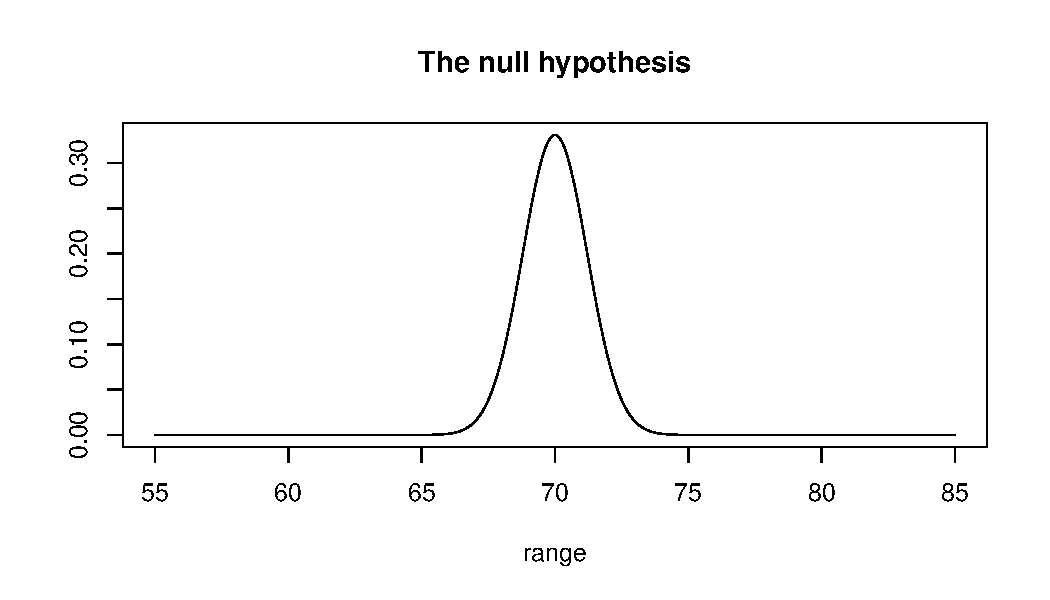
\includegraphics[width=\maxwidth]{figure/unnamed-chunk-40-1} 

\end{knitrout}
\caption{A sampling distribution with mean 70 and $\sigma_{\bar{x}}$ =
1.206.} \label{fig:nullhypexample}
\end{figure}

Suppose now
that we take an actual sample of 11 from a population whose mean $\mu$ is in fact (contra the hypothesis)
60:

\begin{knitrout}
\definecolor{shadecolor}{rgb}{0.969, 0.969, 0.969}\color{fgcolor}\begin{kframe}
\begin{alltt}
\hlstd{sample} \hlkwb{<-} \hlkwd{rnorm}\hlstd{(}\hlnum{11}\hlstd{,}\hlkwc{mean}\hlstd{=}\hlnum{60}\hlstd{,}\hlkwc{sd}\hlstd{=}\hlnum{4}\hlstd{)}
\end{alltt}
\end{kframe}
\end{knitrout}

\begin{knitrout}
\definecolor{shadecolor}{rgb}{0.969, 0.969, 0.969}\color{fgcolor}\begin{kframe}
\begin{alltt}
\hlstd{sample.mean} \hlkwb{<-} \hlkwd{mean}\hlstd{(sample)}
\end{alltt}
\end{kframe}
\end{knitrout}



Inspection of (Figure~\ref{fig:nullhypexample}) shows that, in a world
in which the population mean was really 70, the probability of obtaining a sample whose mean is 60 or something more extreme is extremely low. Intuitively, this sample is ``evidence against the null hypothesis''.

A \textsc{significance test} provides a formal way of quantifying this reasoning. 
The result of such a test yields a probability that
indicates exactly how well or poorly the data and the null hypothesis agree.


\section{The \index{null hypothesis}Null Hypothesis}

While this perfectly symmetrical, intuitive way of viewing things (`evidence for', `evidence against') is on the right track, there is a further fact about the null hypothesis which gives rise to an asymmetry in the way we perform significance tests.

The statement being tested in a significance test--- the
\textsc{null hypothesis}, $H_0$--- is usually formulated in such a way
that the statement represents `no effect'. 
Scientists are usually not so interested in proving `no effect.' This is where the asymmetry comes in: we are usually not interested in finding evidence \emph{for} the null hypothesis, conceived in this way. Rather, we are interested in evidence \emph{against} the null hypothesis. This is what a formal significance test does: it determines whether the result provides sufficient evidence against the null hypothesis for us to reject it.
Note that if it doesn't provide sufficient evidence against the null, we have \emph{not} proved the contrary---we have not `proved the null hypothesis.' We simply don't have enough evidence, \emph{based on this single result}, to reject it. 
\textbf{Absence of evidence is not evidence of absence}.
We come back to this in a later lecture.

In order to achieve a high degree of skepticism about the interpretation of the data, we require the evidence against the null hypothesis to be very great. 
In our current example, you might think the result we obtained, 60, was fairly compelling evidence against it. But how do we quantify this? Intuitively, the further away from the mean of the sampling distribution our data lies, the greater the evidence against it. Statistically significant results reside out in the tails of the distribution. How far out? The actual values and ranges of values we get will vary from experiment to experiment, and statistic to statistic. How can we determine a general rule?

\section{\index{z-scores}z-scores} \label{zscores}

We have already seen that, in a normal distribution, about 95\% of the total probability falls within 2 SD of the mean, and thus 5\% of the probability falls far out in the tails. One way of setting a general rule is to say that if an observed value falls far out in the tail of the distribution, we will consider the result extreme enough to reject the null hypothesis (we can set this threshold anywhere we choose: 95\% is a conventional setting).

Recall our model: we know the sampling distribution we would see in a world in which the null hypothesis is true, in which the population mean is really 70 (and whose population $\sigma$ is known to be 4). We also know this distribution is normal. How many SDs from the mean is our observation? Is it more than 2 SDs?

We need to express the difference between our observation $\bar{x}$ and hypothesized mean of the distribution $\mu_0$ in units of the standard deviation of the distribution: i.e., some number $z$ times
$\sigma_{\bar{x}}$. 
We want to know how many standard deviations (of the sampling distribution of the mean) we are away from the hypothesized mean. 
We want to know this number, call it $z$.

\begin{equation}
\bar{x} - \mu_0 =  z \sigma_{\bar{x}} 
\end{equation}

Solving for $z$:

\begin{align}
z = & \frac{\bar{x} - \mu_0}{\sigma_{\bar{x}}} \\ 
  = & \frac{\bar{x} - \mu_0}{\sigma/\sqrt{n}} 
\end{align}

$z$ is called the \textsc{standardized value} or the \textsc{z-score}. One could imagine computing this standardized version of the sample mean every time we take a sample, in which case we have effectively defined a new statistic. Viewed in this way, the score is also referred to as a \textsc{test statistic}.


Let's make this concrete. Suppose in our current simulation we draw a sample whose mean is precisely 60: then $\bar{x} =  
60, \mu_0 = 70, 
\sigma = 4, n = 11$. So we get:


\begin{align}
z = & \frac{60 - 70}{4/\sqrt{11}} \\
  = & -8.291562
\end{align}

We see that this observation is well beyond 2 SDs from the hypothesized mean (it is -8 SDs away from the hypothesized mean), and thus represents evidence against the null hypothesis.

z-scores are a way of expressing `how far away' from the hypothetical value an observation falls, and for determining if that observation is beyond some accepted threshold. Associated with the z-score is a p-value, which I explain next.

\section{\index{p-values}P-values} \label{pvals}

We reason as follows:
`If, given the null hypothesis, the probability of the obtaining the sample mean that we got, or some value more extreme than that, is less than 0.05, then we reject the null hypothesis.' 

Why do we ask for the probability of the obtaining the sample mean that we got, or some value more extreme than that
Recall that in continuous distributions, the probability of getting exactly a particular value is zero, because the area under the curve at any point (which is its probability) is zero. 

So we cannot use the actual probability of the observed value. But we can ask \emph{how much of
the total probability lies beyond the observed value}, out into the tail of the distribution. In the discrete case this is a sum of probabilities, in the continuous case (normal distribution) an area under the curve. Call $o_1$ the observed value, $o_2$ the next value out, $o_3$ the next, and so on until we exhaust all the possibilities. The sum of these is the probability of a complex event, the probability of `observing the value $o_1$ or a value more extreme.' (Once again, we couch our probability measure in terms of a range of values). 

The smaller this probability, the more extreme the observed sample mean.
We can now say, if this probability is less than $0.05$, we reject the null hypothesis. The technical name for this measure is the \textsc{p-value}.

In short, the p-value of a statistical test is the probability, computed assuming
that $H_0$ is true, that the test statistic would take a
value as extreme
or more extreme than that actually observed. 


\label{pvaluefallacy}
Note that the probability of observing a particular sample
mean (or something more extreme) \textbf{assuming} that
the null hypothesis is true. Abusing notation slightly, we can write this probability
as a conditional probability $P(\hbox{Observed mean or something more extreme}\mid H_0$), or even more succinctly as
$P(x\geq X   \mid H_0)$.\footnote{Technically, it is not correct to call this a conditional probability, because $H_0$ is not a random variable. But we will tell this white lie and keep going.} 

The p-value does \textit{not} measure the
probability of the null hypothesis given the sample mean or something more extreme, $P(H_0 \mid
x\geq X$).  There is a widespread misunderstanding that the
p-value tells you the probability that the null hypothesis is true (in
light of some observation); it doesn't. You can confirm easily that we
cannot ``switch'' conditional probabilities. The probability of the
streets being wet given that rain has fallen $P(\hbox{Wet Streets} \mid
\hbox{Rain})$ (presumably close to 1) is not at all the same as the
probability of rain having fallen given that the streets are wet
$P(\hbox{Rain}\mid \hbox{Wet Streets})$. There are many reasons why the streets may
be wet (street cleaning, burst water pipes, etc.), rain is just one of
the possibilities.


How do we determine this p-value? We simply sum up
(integrate) the area under the normal curve, going out from our observed
value. (For the moment, we are assuming we \emph{know}
the population parameter $\sigma$; we will just make a more realistic assumption soon). We actually have two completely equivalent ways
to do this, since we now have two values (the actual observed value
and its z-score), and two corresponding curves (the  sampling
distribution where the statistic is the sample mean, and the sampling
distribution where the statistic is the standardized mean, the
`z-statistic'). We have seen what the sampling distribution of the sample mean looks like, assuming the null hypothesis is true (i.e. $\mu_0 = 70$, Figure~\ref{fig:nullhypexample}). What is the sampling distribution of the z-statistic under this hypothesis? Let's do a simulation to find out.

In Figure~\ref{fig:sampleMeanVsZ}, we repeat the simulation of sample
means that we carried out at the beginning of the chapter, but now using the parameters of our current null hypothesis $\mu_0 = 70$, $\sigma = 4$, sample size $=11$. But in addition, for each sample we also compute the z-statistic, according to the formula provided above. We also include the corresponding normal curves for reference (recall these represent the limiting case of the simulations). As you can see, the distribution of the z-statistic is normal, with mean $=0$, and SD $=1$. A normal distribution with precisely these parameters is known as the \textsc{standardized normal distribution}.




\begin{figure}[!htbp]
  \centering
\begin{knitrout}
\definecolor{shadecolor}{rgb}{0.969, 0.969, 0.969}\color{fgcolor}
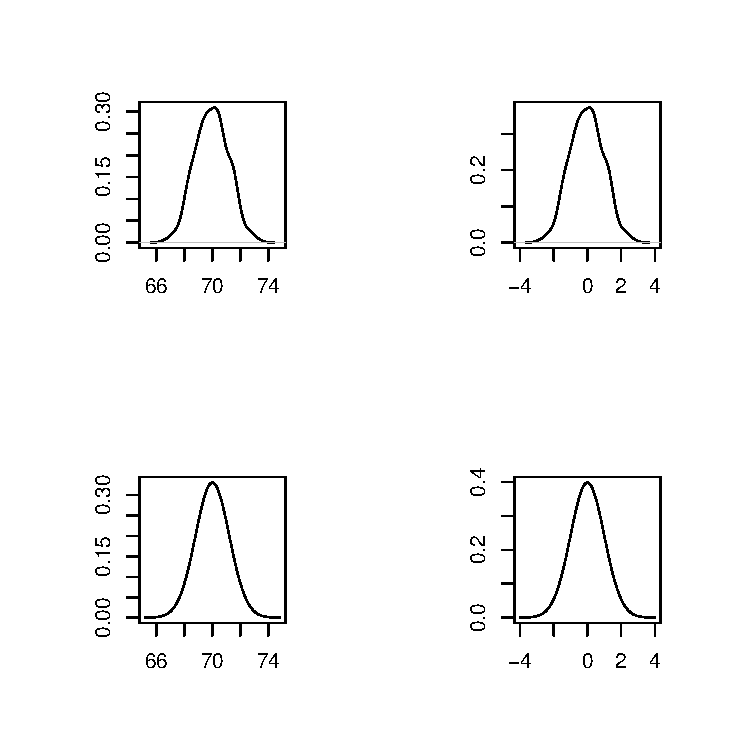
\includegraphics[width=\maxwidth]{figure/unnamed-chunk-43-1} 

\end{knitrout}
\caption{The sampling distribution of the sample mean (left) and its z-statistic (right).}
  \label{fig:sampleMeanVsZ}
\end{figure}

The crucial thing to note is that the area from either value out to the edge, which is the probability of interest, is precisely the same in the two cases, so we can use either. It is traditional to work with the standardized values, for reasons that will become clear very soon.

Recall the z-score for our actual observation was $-8.291562$. This is an extreme value, well beyond 2 standard errors 
from the mean, so we would expect there to be very little probability between it and the left tail of the distribution. We can calculate it directly by integration: 

\begin{knitrout}
\definecolor{shadecolor}{rgb}{0.969, 0.969, 0.969}\color{fgcolor}\begin{kframe}
\begin{alltt}
\hlkwd{integrate}\hlstd{(}\hlkwa{function}\hlstd{(}\hlkwc{x}\hlstd{)} \hlkwd{dnorm}\hlstd{(x,} \hlkwc{mean} \hlstd{=} \hlnum{0}\hlstd{,} \hlkwc{sd} \hlstd{=} \hlnum{1}\hlstd{),} \hlopt{-}\hlnum{Inf}\hlstd{,} \hlopt{-}\hlnum{8.291562}\hlstd{)}
\end{alltt}
\begin{verbatim}
## 5.588542e-17 with absolute error < 4.5e-24
\end{verbatim}
\begin{alltt}
\hlcom{## alternative, more standard way:}
\hlkwd{pnorm}\hlstd{(}\hlkwc{mean}\hlstd{=}\hlnum{0}\hlstd{,}\hlkwc{sd}\hlstd{=}\hlnum{1}\hlstd{,}\hlopt{-}\hlnum{8.291562}\hlstd{)}
\end{alltt}
\begin{verbatim}
## [1] 5.588542e-17
\end{verbatim}
\end{kframe}
\end{knitrout}

This yields a vanishingly small probability. We also get precisely the same result using the actual observed sample mean with the original sampling distribution:

\begin{knitrout}
\definecolor{shadecolor}{rgb}{0.969, 0.969, 0.969}\color{fgcolor}\begin{kframe}
\begin{alltt}
\hlkwd{integrate}\hlstd{(}\hlkwa{function}\hlstd{(}\hlkwc{x}\hlstd{)} \hlkwd{dnorm}\hlstd{(x,} \hlkwc{mean} \hlstd{=} \hlnum{70}\hlstd{,} \hlkwc{sd} \hlstd{=} \hlnum{4}\hlopt{/}\hlkwd{sqrt}\hlstd{(}\hlnum{11}\hlstd{)),} \hlopt{-}\hlnum{Inf}\hlstd{,} \hlnum{60}\hlstd{)}
\end{alltt}
\begin{verbatim}
## 5.588543e-17 with absolute error < 6.2e-20
\end{verbatim}
\begin{alltt}
\hlkwd{pnorm}\hlstd{(}\hlnum{60}\hlstd{,}\hlkwc{mean}\hlstd{=}\hlnum{70}\hlstd{,}\hlkwc{sd}\hlstd{=}\hlnum{4}\hlopt{/}\hlkwd{sqrt}\hlstd{(}\hlnum{11}\hlstd{))}
\end{alltt}
\begin{verbatim}
## [1] 5.588543e-17
\end{verbatim}
\end{kframe}
\end{knitrout}

Suppose now we had observed a sample mean of $67.58$. This is much closer to the hypothetical mean of $70$. The standardized value here is almost exactly $-2.0$:

\begin{knitrout}
\definecolor{shadecolor}{rgb}{0.969, 0.969, 0.969}\color{fgcolor}\begin{kframe}
\begin{alltt}
\hlstd{(}\hlnum{67.58}\hlopt{-}\hlnum{70}\hlstd{)}\hlopt{/}\hlstd{(}\hlnum{4}\hlopt{/}\hlkwd{sqrt}\hlstd{(}\hlnum{11}\hlstd{))}
\end{alltt}
\begin{verbatim}
## [1] -2.006558
\end{verbatim}
\end{kframe}
\end{knitrout}

Integrating under the standardized normal curve we find the following probability:

\begin{knitrout}
\definecolor{shadecolor}{rgb}{0.969, 0.969, 0.969}\color{fgcolor}\begin{kframe}
\begin{alltt}
\hlkwd{integrate}\hlstd{(}\hlkwa{function}\hlstd{(}\hlkwc{x}\hlstd{)} \hlkwd{dnorm}\hlstd{(x,} \hlnum{0}\hlstd{,} \hlnum{1}\hlstd{),} \hlopt{-}\hlnum{Inf}\hlstd{,} \hlopt{-}\hlnum{2.0}\hlstd{)}
\end{alltt}
\begin{verbatim}
## 0.02275013 with absolute error < 1.5e-05
\end{verbatim}
\begin{alltt}
\hlkwd{pnorm}\hlstd{(}\hlopt{-}\hlnum{2}\hlstd{,}\hlkwc{mean}\hlstd{=}\hlnum{0}\hlstd{,}\hlkwc{sd}\hlstd{=}\hlnum{1}\hlstd{)}
\end{alltt}
\begin{verbatim}
## [1] 0.02275013
\end{verbatim}
\end{kframe}
\end{knitrout}

This accords well with our rule-of-thumb. About 95\% of the probability is within 2 standard errors of the mean. The remainder is split into two, one at each end of the distribution, each representing a probability of about 0.025.

In the code above, we have used the \texttt{integrate} function, but the standard way to do this in R (and this is what we will do from now on) is to use \texttt{pnorm}.
For example: we can compute the probability of getting a z-score like $-8.291562$ or smaller using:

\begin{knitrout}
\definecolor{shadecolor}{rgb}{0.969, 0.969, 0.969}\color{fgcolor}\begin{kframe}
\begin{alltt}
\hlkwd{pnorm}\hlstd{(}\hlopt{-}\hlnum{8.291562}\hlstd{)}
\end{alltt}
\begin{verbatim}
## [1] 5.588542e-17
\end{verbatim}
\end{kframe}
\end{knitrout}

Note that I did not specify the mean and sd; this is because the default assumption in this function is that mean is 0 and sd=1.

\section{Hypothesis Testing: A More Realistic Scenario}

In the above example we were able to use the standard deviation of the sampling distribution $\sigma_{\bar{x}}$, because we were given the standard deviation of the population
$\sigma$. As we remarked earlier, in the real world we usually do not know $\sigma$, it's just another unknown parameter of the population. Just as in the case of computing real world confidence intervals, instead of
$\sigma$ we use the estimate $s$; instead of
$\sigma_{\bar{x}}$ we use the estimate $SE_{\bar{x}}$;
instead of the normal distribution we use the t-distribution.

Recall the $z$-score:
\begin{align}
z = & \frac{\bar{x} - \mu_0}{\sigma_{\bar{x}}} \\ 
  = & \frac{\bar{x} - \mu_0}{\sigma/\sqrt{n}} 
\end{align}

And recall our formal definition of a statistic: a number that describes some aspect of the sample. Using this definition, the z-score seems to fail as a statistic, since it makes reference to a population \emph{parameter} $\sigma$. 
But if we now replace that parameter with an estimate $s$ derived from the sample itself, we get the so-called t-statistic:

\begin{align} \label{ttestequation}
t = & \frac{\bar{x} - \mu_0}{SE_{\bar{x}}} \\ 
  = & \frac{\bar{x} - \mu_0}{s/\sqrt{n}} 
\end{align}

This then can also be interpreted as yet another sampling statistic, with its own distribution.

Note that our null hypothesis $H_0$ was that
the hypothesized mean has some specific value $\mu=\mu_0$.
What's the alternative hypothesis? One alternative hypothesis could be that $mu<0$. Another possibility could be that $\mu>0$. A third possibility, which is conventional in the psycholinguistic literature, is that the true value is less than the hypothesized mean \emph{or} the true value is greater than the mean:

\begin{equation}
H_a: \mu\neq \mu_0 \Leftrightarrow \mu < \mu_0 \hbox{ or } \mu > \mu_0
\end{equation}

This means that as evidence for rejection of $H_0$ we will
count extreme values on \emph{both} sides of the sample mean $\bar{x}$. For this reason, the above test is called a \index{significance test, two-sided}\textsc{two-sided significance test} (also known as the \index{significance test, two-tailed}\textsc{two-tailed significance test}). 

In a two-sided test, since the distributions are symmetrical, the p-value will be twice the value of the probability corresponding to the particular t-value we obtain.
If the p-value is
$\leq \alpha$, we say that the data are ``significant'' at level $\alpha$. Purely by convention, $\alpha=0.05$.

\textbf{Important}: The word ``significant'' is very misleading.  It sounds like the finding is ``important'' or ``real''. Researchers also use the word ``reliable'', which is also misleading because it suggests that we know something about reality for sure. As we see in the next chapter, this is not necessarily the case. A lot depends on the properties of the experiment under repeated sampling.

The null hypothesis doesn't need to be that $\mu=0$. If our null hypothesis were that $\mu \geq \mu_0$, then the alternative hypothesis is:

\begin{equation}
H_a:  \mu < \mu_0	
\end{equation}
 
In this situation, we would use a \index{significance test, one-sided}one-sided significance test, reporting the probability in the relevant direction only.

R does everything required for a t-test of significance as follows,
and you can specify (inter alia) what your $\mu_0$ is (note that it
need not be zero), whether it is two-sided or not (see the
documentation for the \texttt{t.test} for details on how to specify
this), and the confidence level (the $\alpha$ level) you desire, as follows:

\begin{knitrout}
\definecolor{shadecolor}{rgb}{0.969, 0.969, 0.969}\color{fgcolor}\begin{kframe}
\begin{alltt}
\hlstd{sample.11} \hlkwb{<-} \hlkwd{rnorm}\hlstd{(}\hlnum{11}\hlstd{,}\hlkwc{mean}\hlstd{=}\hlnum{60}\hlstd{,}\hlkwc{sd}\hlstd{=}\hlnum{4}\hlstd{)}

\hlkwd{t.test}\hlstd{(sample.11,}
       \hlkwc{alternative} \hlstd{=} \hlstr{"two.sided"}\hlstd{,}
       \hlkwc{mu} \hlstd{=} \hlnum{70}\hlstd{,}
       \hlkwc{conf.level} \hlstd{=} \hlnum{0.95}\hlstd{)}
\end{alltt}
\begin{verbatim}
## 
## 	One Sample t-test
## 
## data:  sample.11
## t = -11.359, df = 10, p-value = 4.886e-07
## alternative hypothesis: true mean is not equal to 70
## 95 percent confidence interval:
##  57.82821 61.82023
## sample estimates:
## mean of x 
##  59.82422
\end{verbatim}
\end{kframe}
\end{knitrout}

Experiment with the above code: change the hypothetical mean, change the mean of the sampled population and its SD, change the sample size, etc. In each case, see how the sample mean, the t-score, the p-value and the confidence interval differ. Make sure you understand what the output says---you have the relevant background at this point to do so.

It is also instructive to keep the parameters the same and simply repeat the experiment, taking different random samples each time (effectively, \textsc{replicating} the experiment). Watch how the p-values change, watch how they change from replicate to replicate under different parameter settings. Do you ever find you would accept the null hypothesis when it is in fact false? How likely is it that you would make a mistake like that? This is an issue we will return to in more depth in the next chapter.

The t-value we see above is indeed the t in equation \ref{ttestequation}; we can verify this by doing the calculation by hand:

\begin{knitrout}
\definecolor{shadecolor}{rgb}{0.969, 0.969, 0.969}\color{fgcolor}\begin{kframe}
\begin{alltt}
\hlstd{observed_t}\hlkwb{<-}\hlkwd{round}\hlstd{(((}\hlkwd{mean}\hlstd{(sample.11)}\hlopt{-}\hlnum{70}\hlstd{)}\hlopt{/}\hlkwd{se}\hlstd{(sample.11)),}\hlnum{3}\hlstd{)}
\hlstd{observed_t}
\end{alltt}
\begin{verbatim}
## [1] -11.359
\end{verbatim}
\end{kframe}
\end{knitrout}


\section{Comparing Two Samples}

In one-sample situations our null hypothesis is that the population mean has some specific value $\mu_0$:

\begin{equation}
H_0: \mu=\mu_0
\end{equation}

When we compare samples from two (possibly) different populations, we ask the question: are the
population means identical or not? Our goal now is to
figure out some way to define our null hypothesis in this situation.

Consider this example of a common scenario in experimental research. Let us assume that the 
mean reading times and standard deviations are available 
for children and adults reading English sentences,  
and let us say that we want to know whether children are
faster or slower than adults in terms of reading time.
You probably don't need to do an experiment to answer this question,
but it will do as an illustration of this type of experiment.

We know that, due to the nature of repeated sampling,  
there is bound to be
\emph{some} difference in sample means even if the population means
are identical. We can reframe the research question as follows: is the
difference observed between the two sample means  
consistent or inconsistent with our null hypothesis.  The data are shown in Table~\ref{adultchilddata}.

\begin{table}
\begin{center}
\caption{Hypothetical data showing reading times for adults and children.}
\label{adultchilddata}       % Give a unique label
\begin{tabular}{p{2cm}p{3cm}p{3cm}p{3cm}}
group & sample size $n$ & Mean (secs) & SD \\
\hline
children & $n_1=$ 10 & $\bar{x}_1=30$ & $s_1=43$ \\
adults   & $n_2=$ 20 & $\bar{x}_2=7$ & $s_2=25$ \\
\end{tabular}
\end{center}
\end{table}

Notice a few facts about the data. We have different sample sizes in each case. How will that affect our analysis? Notice too that we have different standard deviations in each case: this makes sense, since children exhibit a wider range of abilities than literate adults. But we now know how great an effect the variability of the data has on statistical inference. How will we cope with these different SD's? Finally, the mean reading times certainly `look'  different. We will quantify this difference with reference to the null hypothesis.

Such research problems have the properties that 
(i) the goal is to compare the responses in two groups;
(ii) each group is considered a sample from a distinct population (a `between-subjects' design);
(iii) the responses in each group are independent of those in the other group; and
(iv) the sample sizes of each group may or may not be different. 

The question now is, given that we have a research question involving two means, how can we formulate the null hypothesis?

\subsection{$H_0$ in \index{two sample problems}Two-sample Problems}

Let us start by saying that the unknown population mean of children is $\mu_1$, and that of adults is $\mu_2$. 
We can state our null hypothesis as follows:

\begin{equation}
H_0: \mu_1 = \mu_2
\end{equation}

\label{twosampleproblemsnull}
Equivalently, we can say that our null hypothesis is that the difference between the two means is zero:

\begin{equation}
H_0: \mu_1 - \mu_2 = 0 = \delta
\end{equation}

We have effectively created a new population parameter $\delta$:

\begin{equation}
H_0: \delta = 0
\end{equation}

We can now define a new \index{statistic}statistic $d = \bar{x}_1 - \bar{x}_2$ and
use that as an estimate of $\delta$, which we've hypothesized to be
equal to zero.  But to do this we need a sampling distribution of the
difference of the two sample means $\bar{x}_1$ and  $\bar{x}_2$.

Let's do a simulation to get an understanding of this approach.
For simplicity we will use the sample means and standard deviations from the example above as our population parameters in the simulation, and we will also use the sample sizes above for the repeated sampling.
Assume a population with $\mu_1 = 30$, $\sigma_1 = 43$, and
another with mean $\mu_2 = 7$, $\sigma_2 = 25$.  So we already know
in this case that the null hypothesis is false, since $\mu_1 \neq \mu_2$.  But let's take 1000
sets of samples of each population, compute the differences in mean in
each set of samples, and plot that distribution of \emph{the differences of
the sample mean}:

%First we simulate 1000 replications from the two populations, compute the difference in means in each of the simulations.


\begin{knitrout}
\definecolor{shadecolor}{rgb}{0.969, 0.969, 0.969}\color{fgcolor}\begin{kframe}
\begin{alltt}
\hlstd{d} \hlkwb{<-} \hlkwd{rep}\hlstd{(}\hlnum{NA}\hlstd{,}\hlnum{1000}\hlstd{)}

\hlkwa{for}\hlstd{(i} \hlkwa{in} \hlnum{1}\hlopt{:}\hlnum{1000}\hlstd{)\{}
  \hlstd{sample1} \hlkwb{<-} \hlkwd{rnorm}\hlstd{(}\hlnum{10}\hlstd{,}\hlkwc{mean}\hlstd{=}\hlnum{30}\hlstd{,}\hlkwc{sd}\hlstd{=}\hlnum{43}\hlstd{)}
  \hlstd{sample2} \hlkwb{<-} \hlkwd{rnorm}\hlstd{(}\hlnum{20}\hlstd{,}\hlkwc{mean}\hlstd{=}\hlnum{7}\hlstd{,}\hlkwc{sd}\hlstd{=}\hlnum{25}\hlstd{)}
  \hlstd{d[i]} \hlkwb{<-} \hlkwd{mean}\hlstd{(sample1)} \hlopt{-} \hlkwd{mean}\hlstd{(sample2)}
\hlstd{\}}
\end{alltt}
\end{kframe}
\end{knitrout}

Note that the vector representing the mean of the
differences vector \texttt{d} is close to the true difference:

\begin{knitrout}
\definecolor{shadecolor}{rgb}{0.969, 0.969, 0.969}\color{fgcolor}\begin{kframe}
\begin{alltt}
\hlnum{30}\hlopt{-}\hlnum{7}
\end{alltt}
\begin{verbatim}
## [1] 23
\end{verbatim}
\begin{alltt}
\hlkwd{mean}\hlstd{(d)}
\end{alltt}
\begin{verbatim}
## [1] 22.51256
\end{verbatim}
\end{kframe}
\end{knitrout}

\noindent
Then we plot the distribution of \texttt{d}; we see a normal distribution  (Figure~\ref{fig:diff}). 



So, the distribution of the differences between the two sample means is normally distributed, and centered around the true difference between
the two populations. It is because of these properties that we can safely take $d$ to be an estimate of $\delta$. How accurate an
estimate is it? In other words, what is the standard deviation of this new sampling distribution? It is clearly dependent on (a function of) the standard deviation of the two populations in some way: 

\begin{equation} \sigma_{\bar{x}_1 - \bar{x}_2} = f(\sigma_1,\sigma_2) \end{equation}

Try increasing one or other or both of the $\sigma$ in the above simulation to see what happens. The precise relationship is fundamentally additive: instead of taking the root of the variance, we take the root of the sum of variances:

\begin{figure}[!htbp]
  \centering
\begin{knitrout}
\definecolor{shadecolor}{rgb}{0.969, 0.969, 0.969}\color{fgcolor}
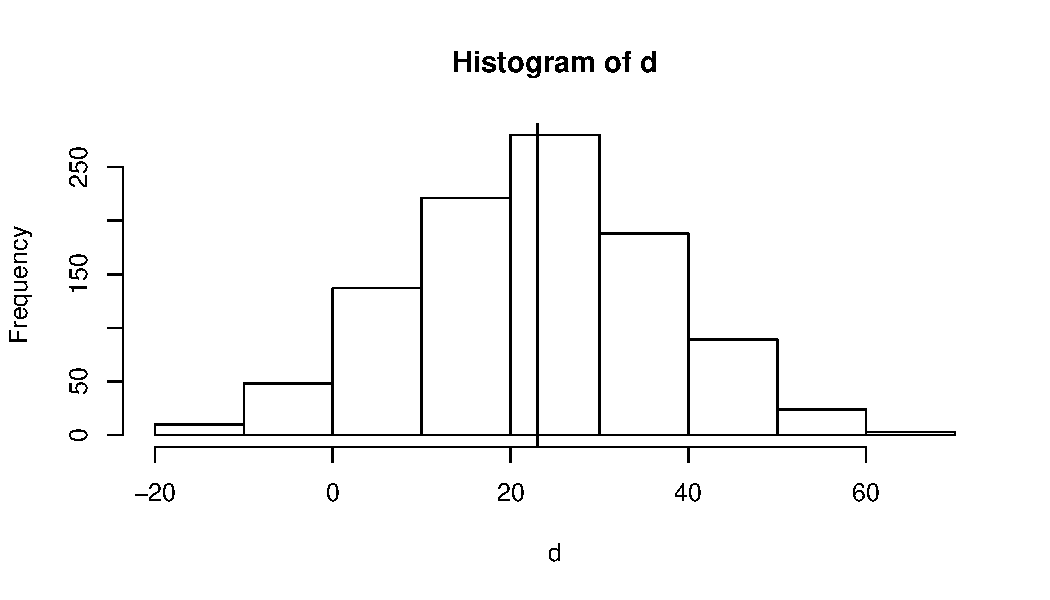
\includegraphics[width=\maxwidth]{figure/unnamed-chunk-53-1} 

\end{knitrout}
  \caption{The distribution of the difference of sample means of two samples. The vertical line shows the true difference between the means (30-7).}
\end{figure}






\begin{equation}
\sigma_{\bar{x}_1 - \bar{x}_2} 
= \sqrt{\frac{\sigma_1^2}{n_1} + \frac{\sigma_2^2}{n_2}} = \sqrt{\frac{43^2}{10} + \frac{25^2}{20}} = 14.702.
\end{equation}

\begin{knitrout}
\definecolor{shadecolor}{rgb}{0.969, 0.969, 0.969}\color{fgcolor}\begin{kframe}
\begin{alltt}
\hlstd{newsigma}\hlkwb{<-}\hlkwd{round}\hlstd{(}\hlkwd{sqrt}\hlstd{((}\hlnum{43}\hlopt{^}\hlnum{2}\hlopt{/}\hlnum{10}\hlstd{)}\hlopt{+}\hlstd{(}\hlnum{25}\hlopt{^}\hlnum{2}\hlopt{/}\hlnum{20}\hlstd{)),}\hlkwc{digits}\hlstd{=}\hlnum{4}\hlstd{)}
\end{alltt}
\end{kframe}
\end{knitrout}


In our single sample, $\bar{x}_1 - \bar{x}_2 = 17$.
The null hypothesis is $\mu_1 - \mu_2 = 0$.
How should we proceed? Is this sample difference sufficiently far away from the hypothetical difference (0) to allow us to reject the null hypothesis? Let's first translate the observed difference 17 into a z-score. Recall how the z-score is calculated:

\begin{equation}
z = \frac{\bar{x} - \mu_0}{\sigma/\sqrt{n}} = \frac{\hbox{sample mean} - \hbox{pop.\ mean}}{\hbox{sd of sampling distribution}}
\end{equation}

If we replace $\bar{x}$ with $d$, and the new standard deviation from the two populations' standard deviations,
we are ready to work out the answer:

\begin{align}
z & = \frac{(\bar{x}_1 - \bar{x}_2) - (\mu_1- \mu_2)}{
\sqrt{\frac{\sigma_1^2}{n_1} + \frac{\sigma_2^2}{n_2}}} \\
  & = \frac{17 - 0}{14.702} \\
  & = 1.1563
\end{align}

Using exactly the same logic as previously, because we don't know the
population parameters in realistic settings, we replace the $\sigma$'s with the sample standard deviations to get the t-statistic:

\begin{align}
t & = \frac{(\bar{x}_1 - \bar{x}_2) - (\mu_1- \mu_2)}{
\sqrt{\frac{s_1^2}{n_1} + \frac{s_2^2}{n_2}}} 
\end{align}

This is the \index{t-statistic, two-sample}\textsc{two-sample} t-\textsc{statistic}. 

So far so good, but we want to now translate this into a p-value, for which we need
the appropriate t-distribution. The problem we face here is that
the degrees of freedom needed for the correct t-distribution are not obvious.
The t-distribution assumes that only one $s$ replaces a single $\sigma$; but
we have two of these.
If $\sigma_1 =\sigma_2$, we could just take a \textit{weighted
    average} of the two sample SDs $s_1$ and $s_2$.

  In our case the correct t-distribution
has $n_1 - 1 + n_2 - 1$ degrees of freedom (the sum of the degrees of freedom
of the two sample variances; see
\cite[422]{rice1995mathematical} for a formal
proof).

In real life we don't know whether $\sigma_1 =\sigma_2$.  One
response would be to err on the side of caution, and simply use
degrees of freedom corresponding to the smaller sample size. Recall
that smaller degrees of freedom reflect greater uncertainty, so the
estimate we get from this simple approach will be a conservative one.

However, in a more sophisticated approach, something called Welch's
correction corrects for possibly unequal variances
in the t-curve. R does this correction for you if you specify that
the variances are to be assumed to be unequal (\texttt{var.equal=FALSE}).

\begin{knitrout}
\definecolor{shadecolor}{rgb}{0.969, 0.969, 0.969}\color{fgcolor}\begin{kframe}
\begin{alltt}
\hlstd{t.test.result}\hlkwb{<-}\hlkwd{t.test}\hlstd{(sample1,sample2,}
       \hlkwc{mu}\hlstd{=}\hlnum{0}\hlstd{,}
       \hlkwc{alternative} \hlstd{=} \hlstr{"two.sided"}\hlstd{,}
        \hlkwc{conf.level} \hlstd{=} \hlnum{0.95}\hlstd{,}\hlkwc{var.equal}\hlstd{=}\hlnum{FALSE}\hlstd{)}
\end{alltt}
\end{kframe}
\end{knitrout}

If you print out the contents of \texttt{t.test.result}, you will see
detailed output. For our current discussion it is sufficient to note
that the t-value is 2.64,
the degrees of freedom are  
15.21 (a value somewhere
between the two sample sizes), 
and the p-value is 0.02. Recall that every
time you run the t-test with newly sampled data (you should try this), your results will be
slightly different; so do not be surprised if you occasionally fail to
find a significant difference between the two groups even though you
already know that in reality there is such a difference. We turn to this
issue in the next lecture.





\chapter{Calibrating the model's properties under repeated sampling}

Let's assume we do an experiment, compute the t-value and p-value for
our sample, and based on these values, reject the null hypothesis. As
we mentioned in the previous chapter, and as you can demonstrate to yourself
through simulated replication of experiments, due to the very nature
of random sampling it is always \emph{possible} to stumble on an unusual sample, one whose statistic just happens to be far from the population parameter. In this case it would, in fact, be an error to reject the hypothesis, though we wouldn't know it. The technical name for this is a \index{error, Type I}\textsc{Type I error}: the null hypothesis is true, but our sample incorrectly leads us to reject it.

The converse can also happen. Suppose the null hypothesis is indeed
false---there is a real difference between two population means, for
example---but the sample values we have happen to be so close to each other that this difference is not detectable. Here, the null hypothesis is false, but we fail to reject it based on our sample. Again, we have
been misled by the sampling process: this is known as a \index{error,
  Type II}\textsc{Type II error}.

In the first case, we would think our experiment had succeeded, publish our result, and move on, unaware of our mistake. Can we minimize this risk? In the second case, we don't get a significant difference, it appears our experiment has failed. Is there some way to minimize the risk? Our problems boil down to controlling \textbf{false discovery rate} (Type I error), and controlling \textbf{false non-discovery rate} (Type II error).

Addressing these questions is of fundamental importance in experimental design. It turns out that a couple of the obvious things we \emph{might} do to improve our experiments have unpleasant implications. For example, we might think that making the probability threshold more stringent---0.01 instead of 0.05, for example---will minimize the chance of error. We pay a price for that, however. The reason is that there is an intimate relationship between the two types of error, and a technique that simply aims to minimize one kind can unwittingly increase the chance of the other. This chapter uses simulation to explore this interaction.

\section{\index{Type I and Type II errors}Type I and Type II Errors}


We fix some conventions first for the text below. Let: $R$ = `Reject the null hypothesis $H_0$'; 
$\neg R$ = `Fail to reject the null hypothesis $H_0$.' These are \textbf{decisions} we make based on an experiment's outcome.

The decision $R$ or $\neg R$ is based on the sample.
Keep in mind that when we do an experiment we don't know whether the null
hypothesis is true or not.

The first step in attempting to minimize error is to have some way to measure it. It turns out we can use probability for this as well: we will use conditional probabilities of the following kind:
Let $P(R\mid H_0)$ = `Probability of rejecting the null
hypothesis \textit{conditional on the assumption that the null hypothesis is in fact true}.'

Let's work through the logical possibilities that could hold: the null
hypothesis could be in fact true or in fact false (but we don't know
which), and in addition our decision could be to accept or reject the
null hypothesis (see Table~\ref{nulltruefalse}). In only two of these
four possible cases do we make the right decision. In the table, think
of $\alpha$ as the threshold probability we have been using all along,
0.05.

\begin{table}
\centering
\caption{The logical possibilities given the two possible situations:
  null hypothesis true ($H_0$) or false  ($\neg H_0$).}
\label{nulltruefalse}       % Give a unique label
\begin{tabular}{p{5cm}p{3cm}p{3cm}}
\hline
Reality: & $H_0$ TRUE & $H_0$ FALSE \\
\hline
Decision from sample is `reject': & $\alpha$ & $1~-~\beta$ \\
                                     & \textbf{Type I error}                         & \textbf{Power} \\                                      
                                     & & \\
\hline
Decision from sample is `accept': & $1 - \alpha$ & $\beta$ \\
                                    &                                 & \textbf{Type II error}\\
\hline
\end{tabular}
\end{table}

As shown in Table~\ref{nulltruefalse}, the probability of a Type I
error $P(R\mid H_0)$ is $\alpha$, conventionally set at
0.05. We will see why this is so shortly. But it immediately follows
that the probability of the logical complement $P(\neg R\mid H_0)$ is
$1-\alpha$. We define the probability of a Type II error $P(\neg
R\mid\neg H_0)$ to be $\beta$ (more on this below), but it immediately
follows that the probability of the logical complement $P(\neg
R\mid\neg H_0) = 1 - \beta$. We call this probability
\textsc{power}. Thus, if we want to decrease the chance of a Type II
error, we need to increase the power of the statistical test.

Let's do some simulations to get a better understanding of these various
definitions. We focus on the case where the null hypothesis is in
fact 
false: there is a real difference between population means.

Assume a population with mean $\mu_1 = 60$, $\sigma_1 = 1$, and another with mean $\mu_2 = 62$, $\sigma_2 = 1$.
In this case we already \textit{know} that the null hypothesis is false.
The distribution corresponding to the null hypothesis is shown in Figure~\ref{fig:nullhyprejectionregion}. It is centered around 0, consistent with the null hypothesis that the difference between the means is 0.

We define a function for easily shading the regions of the plot we are
interested in. The function below, \texttt{shadenormal2}, is a
modified version of the function \texttt{shadenormal.fnc} available
from the package \texttt{languageR}  (you do not
need to load the library \texttt{languageR} to use the function below). 

First, we define a function that will plot Type I error
intervals. This function requires that several parameters be set (our
use of this function will clarify how to use these parameters):


\begin{knitrout}
\definecolor{shadecolor}{rgb}{0.969, 0.969, 0.969}\color{fgcolor}\begin{kframe}
\begin{alltt}
\hlcom{## function for plotting type 1 error.}
\hlstd{plot.type1.error}\hlkwb{<-}\hlkwa{function}\hlstd{(}\hlkwc{x}\hlstd{,}
                           \hlkwc{x.min}\hlstd{,}
                           \hlkwc{x.max}\hlstd{,}
                           \hlkwc{qnts}\hlstd{,}
                           \hlkwc{mean}\hlstd{,}
                           \hlkwc{sd}\hlstd{,}
                           \hlkwc{gray.level}\hlstd{,}\hlkwc{main}\hlstd{,}\hlkwc{show.legend}\hlstd{=}\hlnum{TRUE}\hlstd{)\{}

        \hlkwd{plot}\hlstd{(x,}\hlkwd{dnorm}\hlstd{(x,mean,sd),}
                     \hlkwc{type} \hlstd{=} \hlstr{"l"}\hlstd{,}\hlkwc{xlab}\hlstd{=}\hlstr{""}\hlstd{,}\hlkwc{ylab}\hlstd{=}\hlstr{""}\hlstd{,}\hlkwc{main}\hlstd{=main)}
        \hlkwd{abline}\hlstd{(}\hlkwc{h} \hlstd{=} \hlnum{0}\hlstd{)}

\hlcom{## left side    }
    \hlstd{x1} \hlkwb{=} \hlkwd{seq}\hlstd{(x.min,} \hlkwd{qnorm}\hlstd{(qnts[}\hlnum{1}\hlstd{]), qnts[}\hlnum{1}\hlstd{]}\hlopt{/}\hlnum{5}\hlstd{)}
    \hlstd{y1} \hlkwb{=} \hlkwd{dnorm}\hlstd{(x1, mean, sd)}

    \hlkwd{polygon}\hlstd{(}\hlkwd{c}\hlstd{(x1,} \hlkwd{rev}\hlstd{(x1)),}
            \hlkwd{c}\hlstd{(}\hlkwd{rep}\hlstd{(}\hlnum{0}\hlstd{,} \hlkwd{length}\hlstd{(x1)),} \hlkwd{rev}\hlstd{(y1)),}
            \hlkwc{col} \hlstd{= gray.level)}

\hlcom{## right side            }
    \hlstd{x1} \hlkwb{=} \hlkwd{seq}\hlstd{(}\hlkwd{qnorm}\hlstd{(qnts[}\hlnum{2}\hlstd{]), x.max, qnts[}\hlnum{1}\hlstd{]}\hlopt{/}\hlnum{5}\hlstd{)}
    \hlstd{y1} \hlkwb{=} \hlkwd{dnorm}\hlstd{(x1, mean, sd)}
    \hlkwd{polygon}\hlstd{(}\hlkwd{c}\hlstd{(x1,} \hlkwd{rev}\hlstd{(x1)),}
            \hlkwd{c}\hlstd{(}\hlkwd{rep}\hlstd{(}\hlnum{0}\hlstd{,} \hlkwd{length}\hlstd{(x1)),} \hlkwd{rev}\hlstd{(y1)),}
            \hlkwc{col} \hlstd{= gray.level)}
\hlkwa{if}\hlstd{(show.legend}\hlopt{==}\hlnum{TRUE}\hlstd{)\{}\hlkwd{legend}\hlstd{(}\hlnum{2}\hlstd{,}\hlnum{0.3}\hlstd{,} \hlkwc{legend}\hlstd{=}\hlstr{"Type I error"}\hlstd{,}\hlkwc{fill}\hlstd{=gray.level,}\hlkwc{cex}\hlstd{=}\hlnum{1}\hlstd{)\}}
        \hlstd{\}}
\end{alltt}
\end{kframe}
\end{knitrout}

Next, we define a function for plotting Type I and Type II errors;
this function additionally allows us to specify the mean of the null
hypothesis and the population mean that the sample is drawn from
(\texttt{mean.true}):

\begin{knitrout}
\definecolor{shadecolor}{rgb}{0.969, 0.969, 0.969}\color{fgcolor}\begin{kframe}
\begin{alltt}
\hlstd{plot.type1type2.error}\hlkwb{<-}\hlkwa{function}\hlstd{(}\hlkwc{x}\hlstd{,}
                           \hlkwc{x.min}\hlstd{,}
                           \hlkwc{x.max}\hlstd{,}
                           \hlkwc{qnts}\hlstd{,}
                           \hlkwc{mean.null}\hlstd{,}
                           \hlkwc{mean.true}\hlstd{,}
                           \hlkwc{sd}\hlstd{,}
                           \hlkwc{gray1}\hlstd{,}
                           \hlkwc{gray2}\hlstd{,}\hlkwc{main}\hlstd{,}\hlkwc{show.legend}\hlstd{=}\hlnum{TRUE}\hlstd{)\{}
        \hlcom{## the reality:}
        \hlkwd{plot}\hlstd{(x,} \hlkwd{dnorm}\hlstd{(x,mean.true,sd),}
             \hlkwc{type} \hlstd{=} \hlstr{"l"}\hlstd{,}\hlkwc{ylab}\hlstd{=}\hlstr{""}\hlstd{,}\hlkwc{xlab}\hlstd{=}\hlstr{""}\hlstd{,}\hlkwc{main}\hlstd{=main)}
        \hlcom{## null hypothesis distribution:}
      \hlkwd{lines}\hlstd{(x,}\hlkwd{dnorm}\hlstd{(x,mean.null,sd),}\hlkwc{col}\hlstd{=}\hlstr{"black"}\hlstd{)}
      \hlkwd{abline}\hlstd{(}\hlkwc{h} \hlstd{=} \hlnum{0}\hlstd{)}

    \hlcom{## plot Type II error region: }

        \hlstd{x1} \hlkwb{=} \hlkwd{seq}\hlstd{(}\hlkwd{qnorm}\hlstd{(qnts[}\hlnum{1}\hlstd{]), x.max, qnts[}\hlnum{1}\hlstd{]}\hlopt{/}\hlnum{5}\hlstd{)}
        \hlstd{y1} \hlkwb{=} \hlkwd{dnorm}\hlstd{(x1, mean.true, sd)}

      \hlkwd{polygon}\hlstd{(}\hlkwd{c}\hlstd{(x1,} \hlkwd{rev}\hlstd{(x1)),}
              \hlkwd{c}\hlstd{(}\hlkwd{rep}\hlstd{(}\hlnum{0}\hlstd{,} \hlkwd{length}\hlstd{(x1)),}
              \hlkwd{rev}\hlstd{(y1)),} \hlkwc{col} \hlstd{= gray2)}

    \hlcom{## plot Type I error region assuming alpha 0.05:}

    \hlstd{x1} \hlkwb{=} \hlkwd{seq}\hlstd{(x.min,} \hlkwd{qnorm}\hlstd{(qnts[}\hlnum{1}\hlstd{]), qnts[}\hlnum{1}\hlstd{]}\hlopt{/}\hlnum{5}\hlstd{)}
    \hlstd{y1} \hlkwb{=} \hlkwd{dnorm}\hlstd{(x1, mean.null, sd)}
    \hlkwd{polygon}\hlstd{(}\hlkwd{c}\hlstd{(x1,} \hlkwd{rev}\hlstd{(x1)),} \hlkwd{c}\hlstd{(}\hlkwd{rep}\hlstd{(}\hlnum{0}\hlstd{,} \hlkwd{length}\hlstd{(x1)),} \hlkwd{rev}\hlstd{(y1)),} \hlkwc{col} \hlstd{= gray1)}

    \hlstd{x1} \hlkwb{=} \hlkwd{seq}\hlstd{(}\hlkwd{qnorm}\hlstd{(qnts[}\hlnum{2}\hlstd{]), x.max, qnts[}\hlnum{1}\hlstd{]}\hlopt{/}\hlnum{5}\hlstd{)}
    \hlstd{y1} \hlkwb{=} \hlkwd{dnorm}\hlstd{(x1, mean.null, sd)} \hlcom{## changed}
    \hlkwd{polygon}\hlstd{(}\hlkwd{c}\hlstd{(x1,} \hlkwd{rev}\hlstd{(x1)),} \hlkwd{c}\hlstd{(}\hlkwd{rep}\hlstd{(}\hlnum{0}\hlstd{,} \hlkwd{length}\hlstd{(x1)),} \hlkwd{rev}\hlstd{(y1)),} \hlkwc{col} \hlstd{= gray1)}

\hlkwa{if}\hlstd{(show.legend}\hlopt{==}\hlnum{TRUE}\hlstd{)\{}
    \hlkwd{legend}\hlstd{(}\hlnum{2}\hlstd{,}\hlnum{0.3}\hlstd{,} \hlkwc{legend}\hlstd{=}\hlkwd{c}\hlstd{(}\hlstr{"Type I error"}\hlstd{,}\hlstr{"Type II error"}\hlstd{),}
    \hlkwc{fill}\hlstd{=}\hlkwd{c}\hlstd{(gray1,gray2),}\hlkwc{cex}\hlstd{=}\hlnum{1}\hlstd{)\}}
\hlstd{\}}
\end{alltt}
\end{kframe}
\end{knitrout}

The above two functions are then used within another function,
\texttt{shadenormal2} (below), that plots either the Type I error probability region alone, or both Type I and Type II error probability regions. Playing with the parameter settings in this function allows us to examine the relationship between Type I and II errors.

\begin{knitrout}
\definecolor{shadecolor}{rgb}{0.969, 0.969, 0.969}\color{fgcolor}\begin{kframe}
\begin{alltt}
\hlstd{shadenormal2}\hlkwb{<-}
\hlkwa{function} \hlstd{(}\hlkwc{plot.only.type1}\hlstd{=}\hlnum{TRUE}\hlstd{,}
          \hlkwc{alpha}\hlstd{=}\hlnum{0.05}\hlstd{,}
          \hlkwc{gray1}\hlstd{=}\hlkwd{gray}\hlstd{(}\hlnum{0.3}\hlstd{),} \hlcom{## type I shading}
          \hlkwc{gray2}\hlstd{=}\hlkwd{gray}\hlstd{(}\hlnum{0.7}\hlstd{),} \hlcom{## type II shading}
          \hlkwc{x.min}\hlstd{=}\hlopt{-}\hlnum{6}\hlstd{,}
          \hlkwc{x.max}\hlstd{=}\hlkwd{abs}\hlstd{(x.min),}
          \hlkwc{x} \hlstd{=} \hlkwd{seq}\hlstd{(x.min, x.max,} \hlnum{0.01}\hlstd{),}
          \hlkwc{mean.null}\hlstd{=}\hlnum{0}\hlstd{,}
          \hlkwc{mean.true}\hlstd{=}\hlopt{-}\hlnum{2}\hlstd{,}
          \hlkwc{sd}\hlstd{=}\hlnum{1}\hlstd{,}\hlkwc{main}\hlstd{=}\hlstr{""}\hlstd{,}\hlkwc{show.legend}\hlstd{=}\hlnum{TRUE}\hlstd{)}
\hlstd{\{}

    \hlstd{qnt.lower}\hlkwb{<-}\hlstd{alpha}\hlopt{/}\hlnum{2}
    \hlstd{qnt.upper}\hlkwb{<-}\hlnum{1}\hlopt{-}\hlstd{qnt.lower}
    \hlstd{qnts}\hlkwb{<-}\hlkwd{c}\hlstd{(qnt.lower,qnt.upper)}

    \hlkwa{if}\hlstd{(plot.only.type1}\hlopt{==}\hlnum{TRUE}\hlstd{)\{}

     \hlkwd{plot.type1.error}\hlstd{(x,x.min,x.max,qnts,mean.null,sd,}
     \hlstd{gray1,main,show.legend)}

    \hlstd{\}} \hlkwa{else} \hlstd{\{} \hlcom{## plot type I and type II error regions}

   \hlkwd{plot.type1type2.error}\hlstd{(x,}
                         \hlstd{x.min,}
                         \hlstd{x.max,}
                         \hlstd{qnts,}
                         \hlstd{mean.null,}
                         \hlstd{mean.true,}
                         \hlstd{sd,}
                         \hlstd{gray1,}
                         \hlstd{gray2,main,show.legend)}
     \hlstd{\}}
\hlstd{\}}
\end{alltt}
\end{kframe}
\end{knitrout}



\begin{figure}[!htbp]
  \centering
\begin{knitrout}
\definecolor{shadecolor}{rgb}{0.969, 0.969, 0.969}\color{fgcolor}
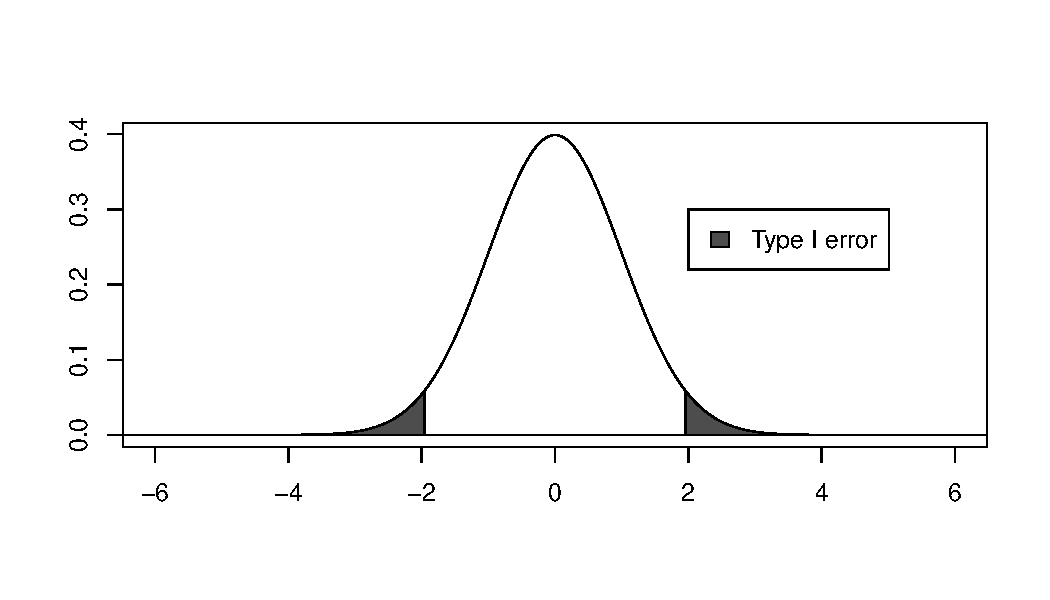
\includegraphics[width=\maxwidth]{figure/unnamed-chunk-60-1} 

\end{knitrout}
  \caption{The distribution corresponding to the null hypothesis,
    along with rejection regions (the Type I error probability region $\alpha$).}
  \label{fig:nullhyprejectionregion}
\end{figure}

The vertical lines in Figure~\ref{fig:nullhyprejectionregion}
represent the 95\% CI, and the shaded areas are the Type I error
regions for a two-sided t-test (with probability in the two regions
summing to $\alpha = 0.05$). A sample mean from one sample taken from
a population with mean zero could possibly lie in this region
(although it's unlikely, given the shape of the distribution), and
based on that one sample, we would incorrectly decide that the null
hypothesis is false when it is actually true. 

In the present example we \emph{know} there is a difference of
$-2$ between the population means. Let's plot the \emph{actual} (as opposed to hypothetical) sampling distribution of mean differences corresponding to this state of the world.



\begin{figure}[!htbp]
\centering 
\begin{knitrout}
\definecolor{shadecolor}{rgb}{0.969, 0.969, 0.969}\color{fgcolor}
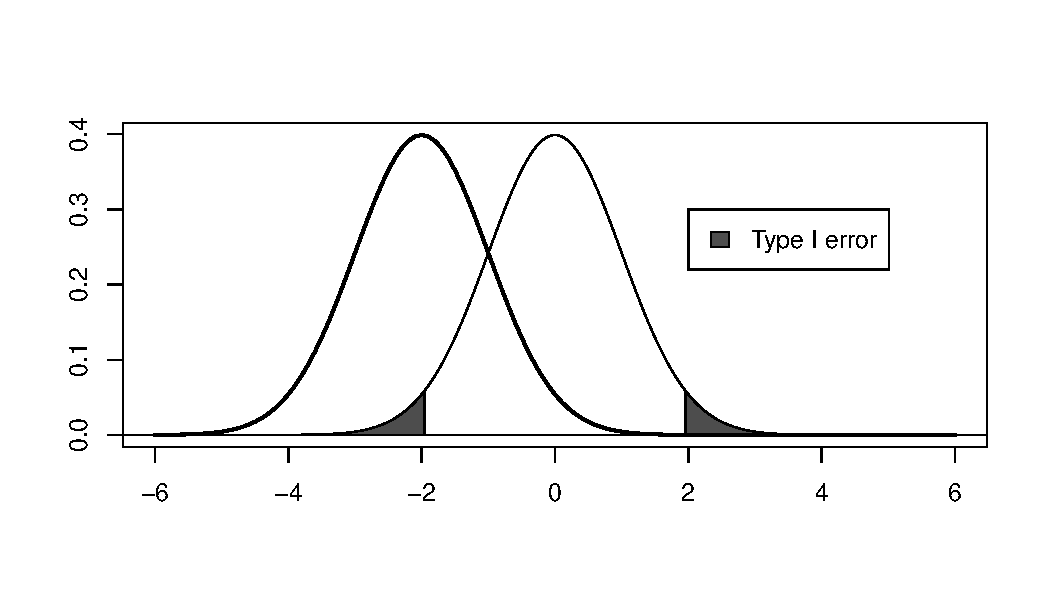
\includegraphics[width=\maxwidth]{figure/unnamed-chunk-61-1} 

\end{knitrout}
  \caption{The distribution corresponding to the null hypothesis and
    the distribution corresponding to the true population scores.}
  \label{fig:nullvstrue}
\end{figure}

Figure~\ref{fig:nullvstrue} shows the distribution corresponding to
the null hypothesis overlaid with the \emph{actual} distribution,
which we \emph{know} is centered around $-2$.  The vertical lines are again the
95\% CI, assuming the null hypothesis is true.

Now let's shade in the region that corresponds to Type II error; see Figure~\ref{fig:nullvstrue2}.
Notice that the values in this region lie \emph{within} the 95\% CI of the null hypothesis. To take a specific example, given that the population means really differ by $-2$, if in our particular sample the difference happened to be $-1$, we would fail to reject $H_0$ even though it is false. This is true for any value in this Type II error range.



\begin{figure}[!htbp]
\centering 
\begin{knitrout}
\definecolor{shadecolor}{rgb}{0.969, 0.969, 0.969}\color{fgcolor}
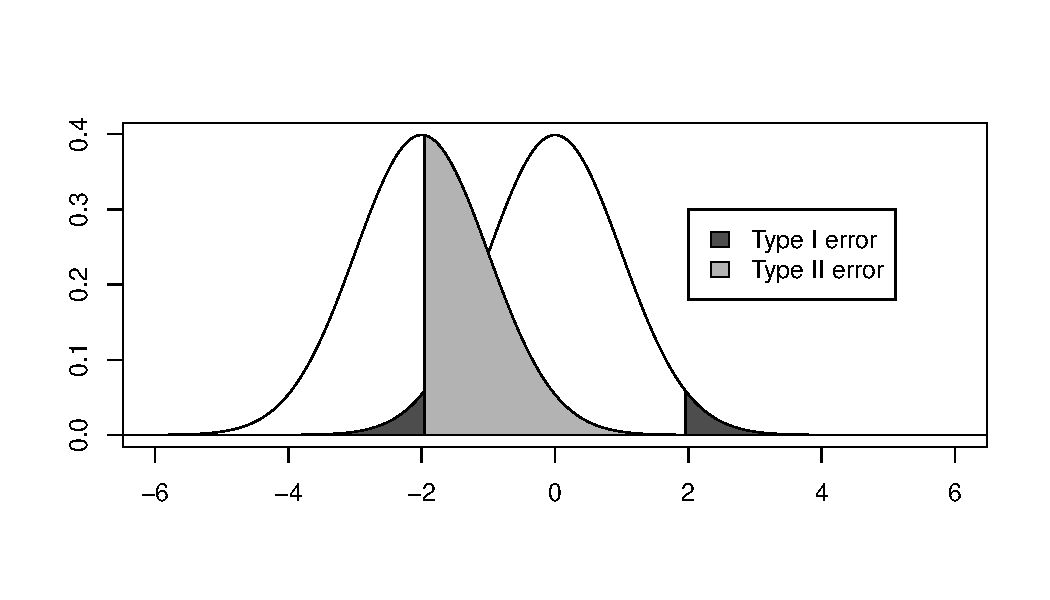
\includegraphics[width=\maxwidth]{figure/unnamed-chunk-62-1} 

\end{knitrout}
  \caption{The distribution corresponding to the true population
    scores along with the confidence intervals from the distribution
    corresponding to the null hypothesis.}
  \label{fig:nullvstrue2}
\end{figure}

Some important insights emerge from  Figure~\ref{fig:nullvstrue2}.  First, if the true
difference between the means had been not $-2$ but $-4$ (i.e., the
\index{effect size} \textsc{effect size} had been greater), then the Type II
error probability ($\beta$) will go down, and therefore power
($1-\beta$) will go up.  Let's confirm this visually (Figure~\ref{fig:nullvstrue3}). 



\begin{figure}[!htbp]
\centering 
\begin{knitrout}
\definecolor{shadecolor}{rgb}{0.969, 0.969, 0.969}\color{fgcolor}
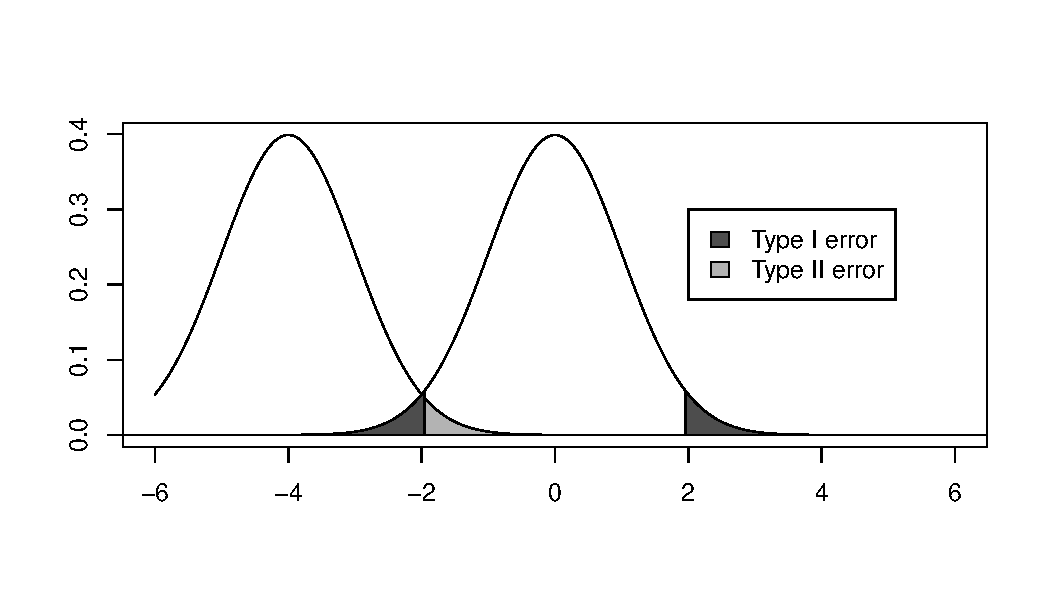
\includegraphics[width=\maxwidth]{figure/unnamed-chunk-63-1} 

\end{knitrout}
  \caption{When the true difference, i.e., the effect size, increases
    from -2 to -4, Type II error probability decreases, and therefore
    power increases. Compare with Figure~\ref{fig:nullvstrue2}.}
  \label{fig:nullvstrue3}
\end{figure}

The second insight is that, for a fixed effect size, if we reduce $\alpha$, we also increase Type II error probability, which reduces power. Suppose $\alpha$ were 0.01; then the Type II error region would be as in Figure~\ref{fig:nullvstrue4}.




\begin{figure}[!htbp]
\centering 
\begin{knitrout}
\definecolor{shadecolor}{rgb}{0.969, 0.969, 0.969}\color{fgcolor}
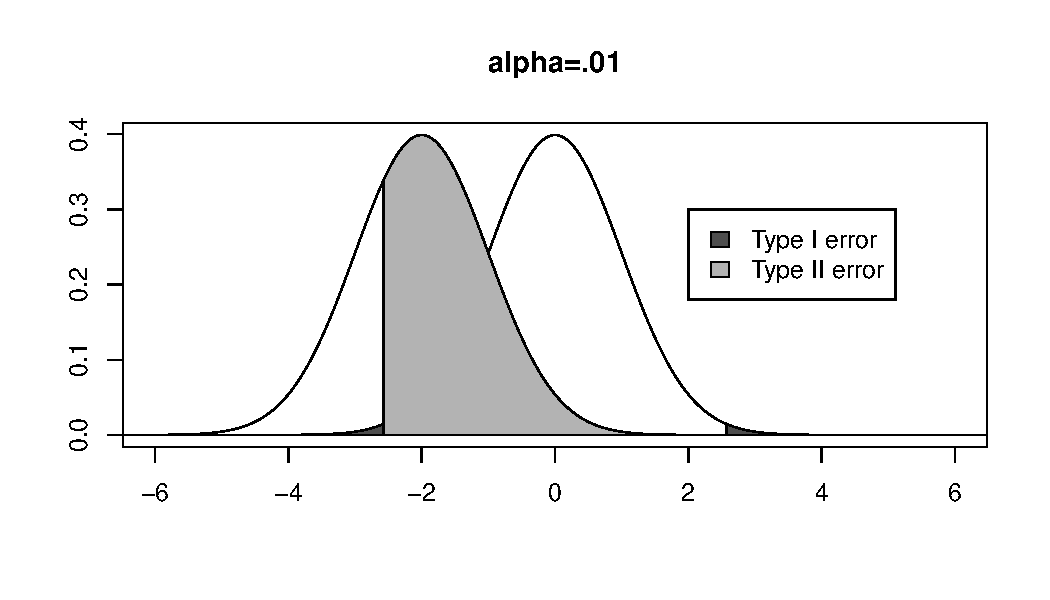
\includegraphics[width=\maxwidth]{figure/unnamed-chunk-64-1} 

\end{knitrout}
  \caption{When we decrease $\alpha$ from 0.05 to 0.01, Type II error probability increases, and therefore power decreases (compare Figure~\ref{fig:nullvstrue2}).}
  \label{fig:nullvstrue4}
\end{figure}

The third insight is that, for a given effect size, as we increase sample size, the 95\%
confidence intervals become tighter. This decreases Type II error
probability, and therefore increases power, as shown in Figure~\ref{fig:nullvstrue5}.



\begin{figure}[!htbp]
\centering 
\begin{knitrout}
\definecolor{shadecolor}{rgb}{0.969, 0.969, 0.969}\color{fgcolor}
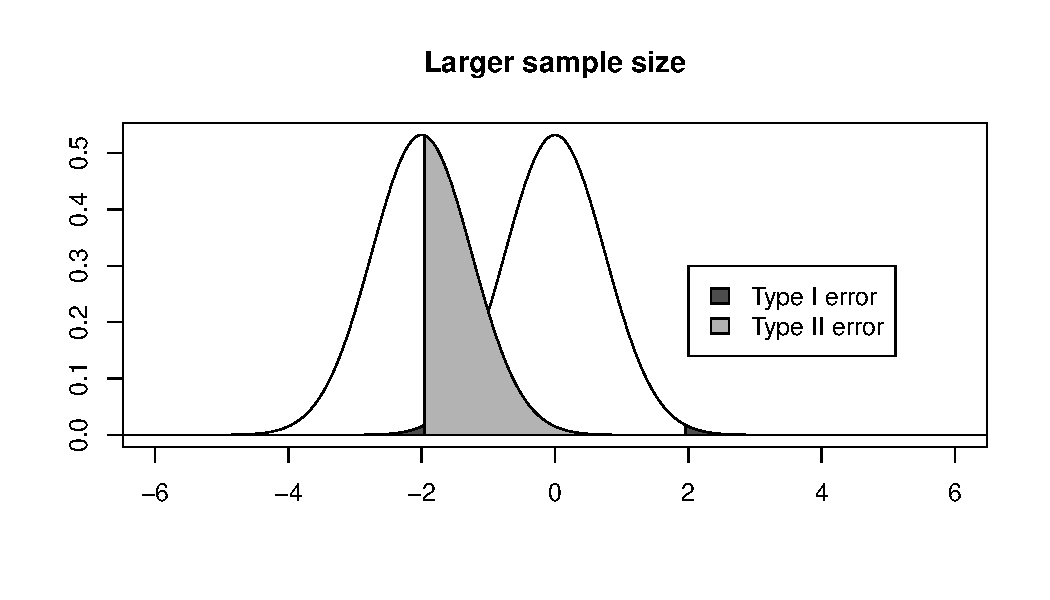
\includegraphics[width=\maxwidth]{figure/unnamed-chunk-65-1} 

\end{knitrout}
  \caption{Increasing sample size will tighten 95\% confidence intervals, decreasing Type II error probability, which increases power (compare with Figure~\ref{fig:nullvstrue2}).}
  \label{fig:nullvstrue5}
\end{figure}

To summarize, the best situation is when we have relatively high power
(low Type II error probability) and low Type I error probability
($\alpha$). By convention, we keep $\alpha$ at 0.05. We usually do not
want to change that: lowering $\alpha$ is costly in the sense that it
reduces power as well, as we just saw. What we do want to ensure is
that power is reasonably high; after all, why would you want to do an
experiment where you have only 50\% power or less? That would mean
that you have an a priori chance of finding a true effect (i.e., an
effect that is actually present in nature) only 50\% of the time or
less. As we just saw, we can increase power by increasing sample size,
and/or by increasing the sensitivity of our experimental design so that
we have larger effect sizes.

Researchers in psycholinguistics and other areas often do experiments
with low power (for logistical or other reasons); it is not unheard of
to publish reading studies (eyetracking or self-paced reading, etc.) or event-related potentials studies with 12 or 20 participants. When power is low, the frequentist method is dead on arrival: a null result tells you nothing if Type I error is high. 
On the other hand, a significant result is guaranteed to be 
exaggerated.  

We would like to make four observations here. These points are also discussed in detail in \cite{VasishthMertzenJaegerGelman2018}.

\begin{enumerate}
	\item
	At least in areas such as psycholinguistics, the null
        hypothesis is, strictly speaking, usually always false: When
        you compare reading times or any other dependent variable in
        two conditions, the a priori chance that the two means to be
        compared are \emph{exactly} identical is zero. The interesting
        question therefore is not whether the null hypothesis is
        false, but what counts as a null effect, and what the estimate of the true effect (the difference between the means) is. 
	\item
	One can in principle nearly always get a statistically
        significant effect given a large enough sample size; the
        question is whether the effect is large enough to be
        theoretically important and whether the difference between
        means has the expected sign. 
      \item Especially in areas like psycholinguistics, replication is
        not given the importance it deserves.  Note that we run a 5\%
        risk of declaring a significant difference when in fact there
        is none (or effectively none, see point 1 above). Replication is the only method to convince
        oneself that an effect is truly present. High power, reasonably large effect sizes, and
        actually replicated results should be your goal in
        experimental science.
A p-value of less than 0.05 does not tell you that you got a ``true effect''. Fisher himself pointed this out:

\begin{quote}
It is usual and convenient for experimenters to take-5 per cent. as a standard level of significance, in the sense that they are prepared to ignore all results which fail to reach this standard, and, by this means, to eliminate from further discussion the greater part of the fluctuations which chance causes have introduced into their experimental results. No such selection can eliminate the whole of the possible effects of chance. coincidence, and if we accept this convenient convention, and agree that an event which would occur by chance only once in 70 trials is decidedly ``significant," in the statistical sense, we thereby admit that \textbf{no isolated experiment, however significant in itself, can suffice for the experimental demonstration of any natural phenomenon; for the ``one chance in a million'' will undoubtedly occur, with no less and no more than its appropriate frequency}, however surprised we may be that it should occur to us. In order to assert that a natural phenomenon is experimentally demonstrable we need, not an isolated record, but a reliable method of procedure. In relation to the test of significance, we may say that a phenomenon is experimentally demonstrable when we know how to conduct an experiment which will rarely fail to give us a statistically significant result.
\end{quote}

\item
	Many researchers also believe that the lower the p-value, the lower the probability that the null hypothesis is true. However, as discussed earlier, this is a misunderstanding that stems from a
failure to attend to the meaning of the p-value.
\end{enumerate}

It follows from the above discussion that if you have a relatively narrow CI, and a nonsignificant result
($p > .05$), you have relatively high power and a relatively low
probability of making a Type II error (accepting the null hypothesis
as true when it is in fact false).
This is particularly important for interpreting null results (results where the p-value is greater than $0.05$).
\cite{hoenigheisey} suggest a heuristic: 
if you have a narrow CI, and a
nonsignificant result, you have some justification for concluding that
the null hypothesis may in fact be effectively true. Conversely, if you have a
wide CI and a nonsignificant result the result really is inconclusive.

\section{Computing sample size for a t-test using R}

Suppose you want to compute the sample size you need to have power 0.8 and alpha 0.05. I look at the paired sample case.

You need to decide on a few things:

\begin{itemize}
\item The magnitude of the effect you expect (based on previous work, or theory): delta (the difference between the means you're comparing)
\item  The standard deviation of the difference that between means that you expect (also based on previous data or theory)
\item Your significance level (alpha)
\item The power you want (APA recommends at least 0.80)
\item Type of t-test (usually a paired t-test in psycholinguistics)
\item The type of alternative hypothesis you have (we will always do the two-sided case)
\end{itemize}

\begin{knitrout}
\definecolor{shadecolor}{rgb}{0.969, 0.969, 0.969}\color{fgcolor}\begin{kframe}
\begin{alltt}
\hlkwd{power.t.test}\hlstd{(}\hlkwc{n} \hlstd{=} \hlkwa{NULL}\hlstd{,} \hlkwc{delta} \hlstd{=} \hlnum{100}\hlstd{,} \hlkwc{sd} \hlstd{=} \hlnum{100}\hlstd{,} \hlkwc{sig.level} \hlstd{=} \hlnum{0.05}\hlstd{,}
             \hlkwc{power} \hlstd{=} \hlnum{0.80}\hlstd{,}
             \hlkwc{type} \hlstd{=} \hlkwd{c}\hlstd{(}\hlstr{"paired"}\hlstd{),}
             \hlkwc{alternative} \hlstd{=} \hlkwd{c}\hlstd{(}\hlstr{"two.sided"}\hlstd{),}
             \hlkwc{strict} \hlstd{=} \hlnum{FALSE}\hlstd{)}
\end{alltt}
\begin{verbatim}
## 
##      Paired t test power calculation 
## 
##               n = 9.937864
##           delta = 100
##              sd = 100
##       sig.level = 0.05
##           power = 0.8
##     alternative = two.sided
## 
## NOTE: n is number of *pairs*, sd is std.dev. of *differences* within pairs
\end{verbatim}
\end{kframe}
\end{knitrout}

The calculation suggests a sample size of 10 (rounding up). For other tests there are comparable functions in R, just look in the R help.

\section{The form of the power function}

Assume that the null hypothesis has mean 93, true sd is 5, and sample size is 20. If the null were true, the rejection region would be bounded by 

\begin{knitrout}
\definecolor{shadecolor}{rgb}{0.969, 0.969, 0.969}\color{fgcolor}\begin{kframe}
\begin{alltt}
\hlkwd{qnorm}\hlstd{(}\hlnum{0.025}\hlstd{,}\hlkwc{mean}\hlstd{=}\hlnum{93}\hlstd{,}\hlkwc{sd}\hlstd{=}\hlnum{5}\hlopt{/}\hlkwd{sqrt}\hlstd{(}\hlnum{20}\hlstd{))}
\end{alltt}
\begin{verbatim}
## [1] 90.80869
\end{verbatim}
\begin{alltt}
\hlkwd{qnorm}\hlstd{(}\hlnum{0.975}\hlstd{,}\hlkwc{mean}\hlstd{=}\hlnum{93}\hlstd{,}\hlkwc{sd}\hlstd{=}\hlnum{5}\hlopt{/}\hlkwd{sqrt}\hlstd{(}\hlnum{20}\hlstd{))}
\end{alltt}
\begin{verbatim}
## [1] 95.19131
\end{verbatim}
\end{kframe}
\end{knitrout}

Intuitively, power will go up if the true value of the mean is far from the hypothesized mean, in either direction (greater than, or less than the hypothesized mean). We can look at how power changes as a function of how far away the true mean is from the hypothesized mean:


\begin{knitrout}
\definecolor{shadecolor}{rgb}{0.969, 0.969, 0.969}\color{fgcolor}\begin{kframe}
\begin{alltt}
\hlstd{sd}\hlkwb{<-}\hlnum{5}
\hlstd{n}\hlkwb{<-}\hlnum{20}
\hlstd{power.fn}\hlkwb{<-}\hlkwa{function}\hlstd{(}\hlkwc{mu}\hlstd{)\{}
\hlcom{## lower and upper bounds of rejection regions}
\hlcom{## defined by null hypothesis mean:}
\hlstd{lower}\hlkwb{<-}\hlkwd{qnorm}\hlstd{(}\hlnum{0.025}\hlstd{,}\hlkwc{mean}\hlstd{=}\hlnum{93}\hlstd{,}\hlkwc{sd}\hlstd{=}\hlnum{5}\hlopt{/}\hlkwd{sqrt}\hlstd{(}\hlnum{20}\hlstd{))}
\hlstd{upper}\hlkwb{<-}\hlkwd{qnorm}\hlstd{(}\hlnum{0.975}\hlstd{,}\hlkwc{mean}\hlstd{=}\hlnum{93}\hlstd{,}\hlkwc{sd}\hlstd{=}\hlnum{5}\hlopt{/}\hlkwd{sqrt}\hlstd{(}\hlnum{20}\hlstd{))}

\hlcom{## lower rejection region:}
\hlstd{z.l}\hlkwb{<-}\hlstd{(lower}\hlopt{-}\hlstd{mu)}\hlopt{/}\hlstd{(sd}\hlopt{/}\hlkwd{sqrt}\hlstd{(n))}
\hlcom{## upper rejection region for given true mu:	}
\hlstd{z.u}\hlkwb{<-}\hlstd{(upper}\hlopt{-}\hlstd{mu)}\hlopt{/}\hlstd{(sd}\hlopt{/}\hlkwd{sqrt}\hlstd{(n))}
\hlcom{## return rejection probability:}
    \hlkwd{return}\hlstd{(}\hlkwd{pnorm}\hlstd{(z.u,}\hlkwc{lower.tail}\hlstd{=F)}\hlopt{+}
          \hlkwd{pnorm}\hlstd{(z.l,}\hlkwc{lower.tail}\hlstd{=T))\}}

\hlcom{## a range of true values:	}
\hlstd{alt}\hlkwb{<-}\hlkwd{seq}\hlstd{(}\hlnum{86}\hlstd{,}\hlnum{100}\hlstd{,}\hlkwc{by}\hlstd{=}\hlnum{0.1}\hlstd{)}
\hlstd{pow}\hlkwb{<-}\hlkwd{power.fn}\hlstd{(alt)}
\hlkwd{plot}\hlstd{(alt,pow,}\hlkwc{type}\hlstd{=}\hlstr{"l"}\hlstd{,}
\hlkwc{xlab}\hlstd{=}\hlstr{"Specific parameters 
     for alternative hypothesis"}\hlstd{,}
     \hlkwc{ylab}\hlstd{=}\hlstr{"Power"}\hlstd{,}\hlkwc{main}\hlstd{=}\hlstr{"Power function 
     for H0: mu=93"}\hlstd{)}
\end{alltt}
\end{kframe}
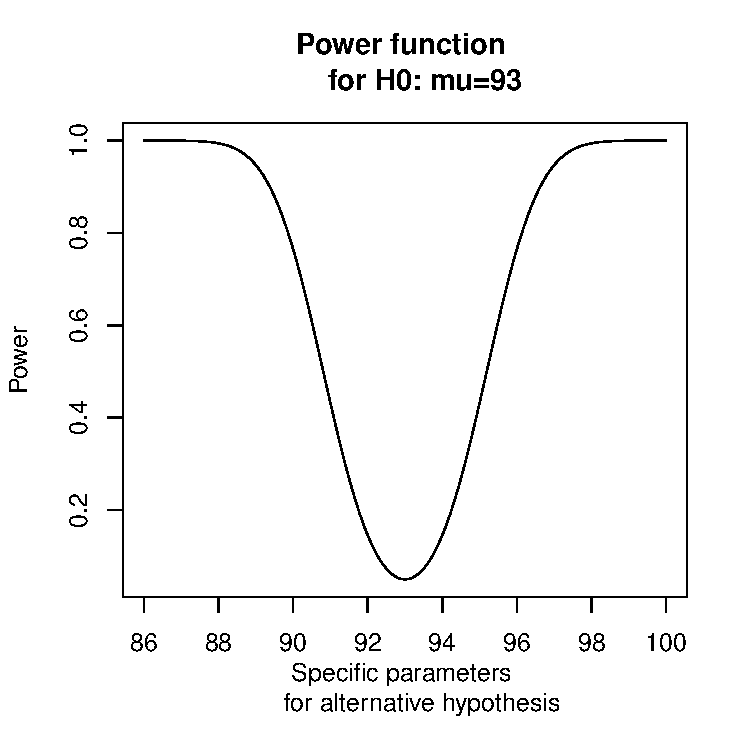
\includegraphics[width=\maxwidth]{figure/unnamed-chunk-68-1} 

\end{knitrout}

What do you think would be the shape of this function if you increased sample size? What would be the shape if you increased standard deviation?
First try to sketch the shapes on paper, and then use the above function to display the shape.

\section{Computing the power function (optional reading)}

You don't need to know this material, but I added it in case anyone is interested in finding out how exactly the power calculation is done.

As an example, let $H_0: \mu = 93$, and let $H_1: \mu \neq 93$. Assume that population sd $\sigma$ and sample size $n$ are given. Note that in realistic situations we don't know $\sigma$ but we can estimate it using $s$.

We can get a sample mean that is greater than $\mu$ or one that is smaller than $\mu$. Call these $\bar{x}_g$ and $\bar{x}_s$ respectively. 

In the case where we know $\sigma$, the test \textbf{under the null hypothesis} is:

\begin{equation}
\frac{\bar{x}_g-93}{\sigma / \sqrt{n}} > 1.96
\quad \hbox{ or }
\quad
\frac{\bar{x}_s-93}{\sigma / \sqrt{n}} > -1.96
\end{equation}

Solving for the two $\bar{x}$'s, we get:

\begin{equation}
\bar{x}_g > 1.96\frac{\sigma}{\sqrt{n}} + 93  
\quad \hbox{ or }
\quad
\bar{x}_s > -1.96\frac{\sigma}{\sqrt{n}} + 93  
\end{equation}

Now, power is the probability of rejecting the null hypothesis when the mean is whatever the alternative hypothesis mean is (some specific value $\mu$).

That, the test \textbf{under the alternative hypothesis} is:

\begin{equation}
\frac{\bar{x}_g - \mu}{\sigma / \sqrt{n}} > 1.96 
\quad
or 
\quad 
\frac{\bar{x}_s - \mu}{\sigma / \sqrt{n}} < -1.96 
\end{equation}

We can replace the $\bar{x}_g$ with its full form, and do the same with $\bar{x}_s$.

\begin{equation}
\frac{1.96\frac{\sigma}{\sqrt{n}} + 93 - \mu}{\sigma / \sqrt{n}} > 1.96 
\quad
or 
\quad 
\frac{-1.96\frac{\sigma}{\sqrt{n}} + 93 - \mu}{\sigma / \sqrt{n}} < -1.96 
\end{equation}

We can rewrite the above as:

\begin{equation}
\frac{1.96\frac{\sigma}{\sqrt{n}} - (\mu - 93)}{\sigma / \sqrt{n}} > 1.96 
\quad
or 
\quad 
\frac{-1.96\frac{\sigma}{\sqrt{n}} - (\mu - 93)}{\sigma / \sqrt{n}} < -1.96 
\end{equation}

Simplifying:

\begin{equation}
1.96 - \frac{(\mu - 93)}{\sigma / \sqrt{n}} > 1.96 
\quad
or 
\quad 
-1.96 - \frac{(\mu - 93)}{\sigma / \sqrt{n}} < -1.96 
\end{equation}

This is now easy to solve! We will use R's pnorm function in the equation below, which is the cumulative distribution function for the normal distribution. 
We can rewrite the above expression as:

\begin{equation}
[1 - pnorm(1.96 - \frac{(\mu - 93)}{\sigma / \sqrt{n}})] + pnorm(-1.96 - \frac{(\mu - 93)}{\sigma / \sqrt{n}})
\end{equation}

The above equation allows us to 

\begin{itemize}
\item
compute sample size for any given null (here 93) and alternative hypotheses, provided I have the population standard deviation.
\item 
compute power given a null and alternative hypothesis, population standard deviation, and sample size.
\end{itemize}

Example: 
suppose I need power of $0.99$ for
$H_0: \mu=93$ 
and $H_1: \mu=98$, $\sigma=5$. 

For this example, what sample size do I need? I take the above equation and fill in the values:

\begin{equation}
[1 - pnorm(1.96 - \frac{(98 - 93)}{5 / \sqrt{n}})] + pnorm(-1.96 - \frac{(98 - 93)}{5 / \sqrt{n}})
\end{equation}

Simplifying, this gives us:

\begin{equation}
[1 - pnorm(1.96 - \sqrt{n})] + pnorm(-1.96 - \sqrt{n})
\end{equation}

Note that the second term will be effectively zero for some reasonable n like 10:

\begin{knitrout}
\definecolor{shadecolor}{rgb}{0.969, 0.969, 0.969}\color{fgcolor}\begin{kframe}
\begin{alltt}
\hlkwd{pnorm}\hlstd{(}\hlopt{-}\hlnum{1.96}\hlopt{-}\hlkwd{sqrt}\hlstd{(}\hlnum{10}\hlstd{))}
\end{alltt}
\begin{verbatim}
## [1] 1.509335e-07
\end{verbatim}
\end{kframe}
\end{knitrout}

So we can concentrate on the first term:

\begin{equation}
[1 - pnorm(1.96 - \sqrt{n})]
\end{equation}

If the above has to be equal to $0.99$, then 

\begin{equation}
pnorm(1.96 - \sqrt{n})=0.01
\end{equation}

So, we just need to find the value of the z-score that will give us a probability of approximately 0.01. You can do this analytically (exercise), but you could also play with some values of n to see what you get. The answer is $n=18$.

\begin{knitrout}
\definecolor{shadecolor}{rgb}{0.969, 0.969, 0.969}\color{fgcolor}\begin{kframe}
\begin{alltt}
\hlkwd{pnorm}\hlstd{(}\hlnum{1.96}\hlopt{-}\hlkwd{sqrt}\hlstd{(}\hlnum{18}\hlstd{))}
\end{alltt}
\begin{verbatim}
## [1] 0.01122577
\end{verbatim}
\end{kframe}
\end{knitrout}

\section{Stopping rules}

Psycholinguists and psychologists often adopt the following type of data-gathering procedure.
The experimenter gathers $n$ data points, then checks for significance ($p<0.05$ or not). If it's not significant, he gets more data ($n$ more data points). Since time and money are limited, he might decide to stop anyway at sample size, say, some multiple of $n$. 
One can play with different scenarios here. A typical $n$ might be $15$.

This approach would give us a range of p-values under repeated sampling. Theoretically, under the standard assumptions of frequentist methods, we expect a Type I error to be $0.05$. This is the case in standard analyses (I also track the t-statistic, in order to compare it with my stopping rule code below).

\begin{knitrout}
\definecolor{shadecolor}{rgb}{0.969, 0.969, 0.969}\color{fgcolor}\begin{kframe}
\begin{alltt}
\hlcom{##Standard:}
\hlstd{pvals}\hlkwb{<-}\hlkwa{NULL}
\hlstd{tstat_standard}\hlkwb{<-}\hlkwa{NULL}
\hlstd{n}\hlkwb{<-}\hlnum{10}
\hlstd{nsim}\hlkwb{<-}\hlnum{1000}
\hlcom{## assume a standard dev of 1:}
\hlstd{stddev}\hlkwb{<-}\hlnum{1}
\hlstd{mn}\hlkwb{<-}\hlnum{0}
\hlkwa{for}\hlstd{(i} \hlkwa{in} \hlnum{1}\hlopt{:}\hlstd{nsim)\{}
  \hlstd{samp}\hlkwb{<-}\hlkwd{rnorm}\hlstd{(n,}\hlkwc{mean}\hlstd{=mn,}\hlkwc{sd}\hlstd{=stddev)}
  \hlstd{pvals[i]}\hlkwb{<-}\hlkwd{t.test}\hlstd{(samp)}\hlopt{$}\hlstd{p.value}
  \hlstd{tstat_standard[i]}\hlkwb{<-}\hlkwd{t.test}\hlstd{(samp)}\hlopt{$}\hlstd{statistic}
\hlstd{\}}

\hlcom{## Type I error rate: about 5% as theory says:}
\hlkwd{table}\hlstd{(pvals}\hlopt{<}\hlnum{0.05}\hlstd{)[}\hlnum{2}\hlstd{]}\hlopt{/}\hlstd{nsim}
\end{alltt}
\begin{verbatim}
##  TRUE 
## 0.052
\end{verbatim}
\end{kframe}
\end{knitrout}

But the situation quickly deteriorates as soon as adopt the strategy I outlined above. I will also track the distribution of the t-statistic below.

\begin{knitrout}
\definecolor{shadecolor}{rgb}{0.969, 0.969, 0.969}\color{fgcolor}\begin{kframe}
\begin{alltt}
\hlstd{pvals}\hlkwb{<-}\hlkwa{NULL}
\hlstd{tstat}\hlkwb{<-}\hlkwa{NULL}
\hlcom{## how many subjects can I run?}
\hlstd{upper_bound}\hlkwb{<-}\hlstd{n}\hlopt{*}\hlnum{6}

\hlkwa{for}\hlstd{(i} \hlkwa{in} \hlnum{1}\hlopt{:}\hlstd{nsim)\{}
\hlcom{## at the outset we have no significant result:}
  \hlstd{significant}\hlkwb{<-}\hlnum{FALSE}
\hlcom{## null hyp is going to be true,}
\hlcom{## so any rejection is a mistake.}
\hlcom{## take sample:}
  \hlstd{x}\hlkwb{<-}\hlkwd{rnorm}\hlstd{(n,}\hlkwc{mean}\hlstd{=mn,}\hlkwc{sd}\hlstd{=stddev)}
\hlkwa{while}\hlstd{(}\hlopt{!}\hlstd{significant} \hlopt{&} \hlkwd{length}\hlstd{(x)}\hlopt{<}\hlstd{upper_bound)\{}
  \hlcom{## if not significant:}
\hlkwa{if}\hlstd{(}\hlkwd{t.test}\hlstd{(x)}\hlopt{$}\hlstd{p.value}\hlopt{>}\hlnum{0.05}\hlstd{)\{}
  \hlcom{## get more data:}
  \hlstd{x}\hlkwb{<-}\hlkwd{append}\hlstd{(x,}\hlkwd{rnorm}\hlstd{(n,}\hlkwc{mean}\hlstd{=mn,}\hlkwc{sd}\hlstd{=stddev))}
  \hlcom{## otherwise stop:}
\hlstd{\}} \hlkwa{else} \hlstd{\{significant}\hlkwb{<-}\hlnum{TRUE}\hlstd{\}}
\hlstd{\}}
\hlcom{## will be either significant or not:}
\hlstd{pvals[i]}\hlkwb{<-}\hlkwd{t.test}\hlstd{(x)}\hlopt{$}\hlstd{p.value}
\hlstd{tstat[i]}\hlkwb{<-}\hlkwd{t.test}\hlstd{(x)}\hlopt{$}\hlstd{statistic}
\hlstd{\}}

\hlcom{## Type I error rate:}
\hlcom{## much higher than 5%:}
\hlkwd{table}\hlstd{(pvals}\hlopt{<}\hlnum{0.05}\hlstd{)[}\hlnum{2}\hlstd{]}\hlopt{/}\hlstd{nsim}
\end{alltt}
\begin{verbatim}
##  TRUE 
## 0.169
\end{verbatim}
\end{kframe}
\end{knitrout}

Now let's compare the distribution of the t-statistic in the standard case vs with the above stopping rule:

\begin{knitrout}
\definecolor{shadecolor}{rgb}{0.969, 0.969, 0.969}\color{fgcolor}\begin{kframe}
\begin{alltt}
\hlkwd{hist}\hlstd{(tstat_standard,}\hlkwc{main}\hlstd{=}\hlstr{"The t-distributions for the standard case (white) \textbackslash{}n
     vs the stopping rule (gray)"}\hlstd{,}\hlkwc{freq}\hlstd{=F)}
\hlkwd{hist}\hlstd{(tstat,}\hlkwc{add}\hlstd{=T,}\hlkwc{col}\hlstd{=}\hlstr{"#0000ff22"}\hlstd{,}\hlkwc{freq}\hlstd{=F)}
\end{alltt}
\end{kframe}
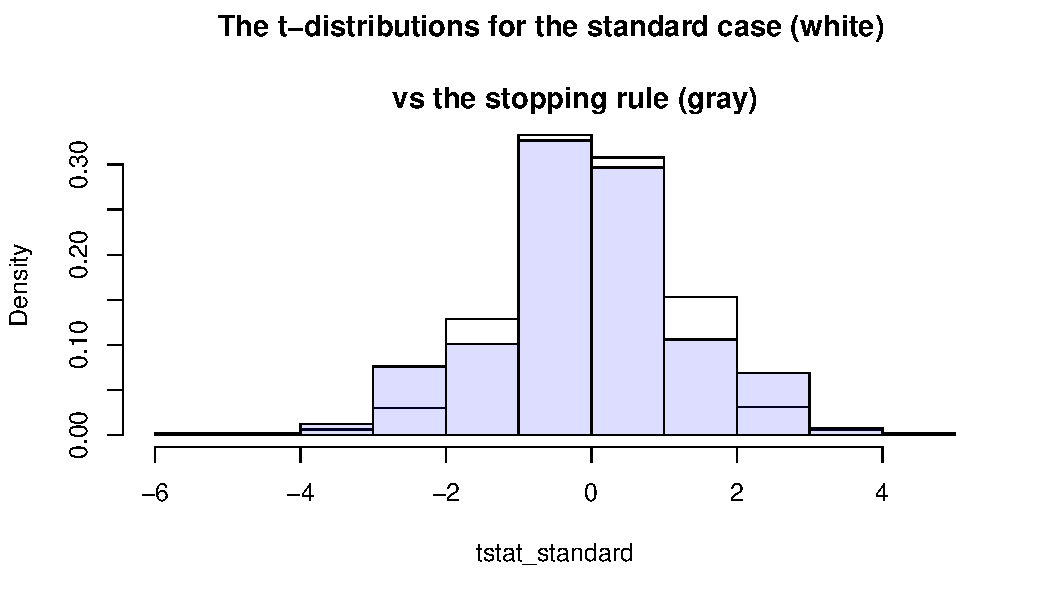
\includegraphics[width=\maxwidth]{figure/unnamed-chunk-73-1} 

\end{knitrout}

We get fatter tails with the above stopping rule. Thus, this common strategy in psycholinguistics of running until significance is reached is at best a questionable research practice, and comes dangerously close to being classified as scientific misconduct.

One should fix one's sample size in advance based on a prospective  power analysis, not deploy a stopping rule like the one above; if we used such a stopping rule, we are much more likely to incorrectly declare a result as statistically significant.

Nevertheless, it is important not to unncessarily get subjects to do an experiment when the results are already clear. In order to collect subjects efficiently, one can decide on a data collection plan, deciding in advance how many times one will check for significance. \cite{pocock2013clinical} explains how to correct $\alpha$ for such a procedure. A better way (in my opinion) is to switch to Bayesian adaptive methods. See Experiment 7 in \cite{VasishthMertzenJaegerGelman2018} for an example.

%This strategy of p-value dependent stopping changes the distribution of the sampling distribution of the means.
%Crucially, the central limit theorem no longer applies.

%The t-test statistic you build from your experiment is distributed as:

%$
%\prod_{i=1}^{10m} \phi(x_i) \times %\prod_{j=1}^{m-1} I_{t(x_1,\ldots,x_{10j})>.05} \times
%I_{t(x_1,\ldots,x_{10j})<.05}
%$

%if $10m<60$ and from

%$
%\prod_{i=1}^{60} \phi(x_i) \times \prod_{j=1}^{5} I_{t(x_1,\ldots,x_{10j})>.05}
%$
%otherwise.



\chapter{Linear models}

\section{Introduction}

\subsection{Example: Subject and object relative clauses}

As a concrete example, consider a classic question from the psycholinguistics literature: are subject relatives easier to process than object relatives? The data come from Experiment 1 in a well-known paper by Grodner and Gibson \cite{grodner}.

In two important papers, Gibson and colleagues \cite{gibson00} and \cite{grodner} argued that object relative clause sentences are more difficult to process than subject relative clause sentences because the distance between the relative clause verb \textit{sent} and the head noun phrase of the relative clause, \textit{reporter}, is longer in object vs subject relatives. Examples are shown below.

(1a) The reporter who the photographer sent to the editor was hoping for a good story. (object relative)

(1b) The reporter who sent the photographer to the editor was hoping for a good story. (subject relative)

The underlying explanation that Grodner and Gibson provided has to do with memory processes: shorter linguistic dependencies are easier to process due to either reduced interference or decay, or both. For implemented computational models that investigate closely related issues, see \cite{lewisvasishth:cogsci05,EngelmannJaegerVasishthSubmitted2018}.

In the Grodner and Gibson data, the dependent measure is reading time at the relative clause verb, in milliseconds. We are expecting longer reading times in object relatives sentences compared to subject relatives.

First, load and reformat the data:




Each subject is seeing 8 items per condition:

\begin{knitrout}
\definecolor{shadecolor}{rgb}{0.969, 0.969, 0.969}\color{fgcolor}\begin{kframe}
\begin{alltt}
\hlkwd{head}\hlstd{(}\hlkwd{xtabs}\hlstd{(}\hlopt{~}\hlstd{subject}\hlopt{+}\hlstd{condition,gge1crit))}
\end{alltt}
\begin{verbatim}
##        condition
## subject objgap subjgap
##       1      8       8
##       2      8       8
##       3      8       8
##       4      8       8
##       5      8       8
##       6      8       8
\end{verbatim}
\end{kframe}
\end{knitrout}

That is, there are 16 items, and 42 subjects, and two conditions.

Isolate the relevant columns, and aggregate the data such that we have one set of paired data for each subject (instead of 8 pairs). (This aggregation is a common way to do data analysis in psycholinguistics. We will use a better method in the next chapter.)

\begin{knitrout}
\definecolor{shadecolor}{rgb}{0.969, 0.969, 0.969}\color{fgcolor}\begin{kframe}
\begin{alltt}
\hlstd{dat}\hlkwb{<-}\hlstd{gge1crit[,}\hlkwd{c}\hlstd{(}\hlnum{1}\hlstd{,}\hlnum{2}\hlstd{,}\hlnum{3}\hlstd{,}\hlnum{6}\hlstd{)]}
\hlkwd{head}\hlstd{(dat)}
\end{alltt}
\begin{verbatim}
##    subject item condition rawRT
## 6        1    1    objgap   320
## 19       1    2   subjgap   424
## 34       1    3    objgap   309
## 49       1    4   subjgap   274
## 68       1    5    objgap   333
## 80       1    6   subjgap   266
\end{verbatim}
\begin{alltt}
\hlstd{dat}\hlkwb{<-}\hlkwd{aggregate}\hlstd{(}\hlkwc{data}\hlstd{=gge1crit,rawRT}\hlopt{~}\hlstd{subject}\hlopt{+}
                           \hlstd{condition,}
          \hlkwc{FUN}\hlstd{=mean)}
\hlkwd{head}\hlstd{(dat)}
\end{alltt}
\begin{verbatim}
##   subject condition   rawRT
## 1       1    objgap 335.000
## 2       2    objgap 419.375
## 3       3    objgap 247.250
## 4       4    objgap 616.375
## 5       5    objgap 395.750
## 6       6    objgap 330.250
\end{verbatim}
\end{kframe}
\end{knitrout}

\subsubsection{The simple linear model}

Suppose $y$ is a vector of continuous responses; assume for now that it is coming from a normal distribution. In other words, the random variable $Y$ has the pdf:

\begin{equation}
Y \sim Normal(\mu,\sigma)
\end{equation}

A crucial assumption here is that the vector of data $y$ is \textbf{independent and identically distributed}. This implies that if we have $n$ data points, $y_1,y_2,\dots,y_n$, each one of these data points has the same distribution, and is indepenent from each other. We write this assumption into the equation as follows:

\begin{equation}
Y \overset{iid}{\sim} Normal(\mu,\sigma)
\end{equation}



One can equivalently write the above model as a so-called linear model (I'm dropping the expression iid, as it's understood in this chapter from this point on):

\begin{equation}
y = \mu + \varepsilon \hbox{ where } \varepsilon \sim Normal(0,\sigma)
\end{equation}

The goal is to estimate two parameters, $\mu,\sigma$. 
Here, we will have the R function lm do the estimation.

\begin{knitrout}
\definecolor{shadecolor}{rgb}{0.969, 0.969, 0.969}\color{fgcolor}\begin{kframe}
\begin{alltt}
\hlstd{m}\hlkwb{<-}\hlkwd{lm}\hlstd{(rawRT}\hlopt{~}\hlnum{1}\hlstd{,dat)}
\hlkwd{summary}\hlstd{(m)}
\end{alltt}
\begin{verbatim}
## 
## Call:
## lm(formula = rawRT ~ 1, data = dat)
## 
## Residuals:
##     Min      1Q  Median      3Q     Max 
## -252.22 -124.59  -54.40   59.47  904.41 
## 
## Coefficients:
##             Estimate Std. Error t value Pr(>|t|)    
## (Intercept)   420.22      22.59   18.61   <2e-16 ***
## ---
## Signif. codes:  0 '***' 0.001 '**' 0.01 '*' 0.05 '.' 0.1 ' ' 1
## 
## Residual standard error: 207 on 83 degrees of freedom
\end{verbatim}
\end{kframe}
\end{knitrout}

The Intercept shown above is an estimate of the grand mean from the data:

\begin{knitrout}
\definecolor{shadecolor}{rgb}{0.969, 0.969, 0.969}\color{fgcolor}\begin{kframe}
\begin{alltt}
\hlkwd{round}\hlstd{(}\hlkwd{mean}\hlstd{(dat}\hlopt{$}\hlstd{rawRT),}\hlnum{2}\hlstd{)}
\end{alltt}
\begin{verbatim}
## [1] 420.22
\end{verbatim}
\end{kframe}
\end{knitrout}

But this model is actually not the relevant one for these data: It doesn't answer our question, which is ``are SRs easier to process than ORs?''

To answer this question, we have to think about our data as containing not one vector of $y$ responses, but  two vectors. The first vector, of length $n_{obj}=42$, is:

\begin{equation}
y_{obj} \sim Normal(\mu_{obj},\sigma)
\end{equation}


and the second vector, also of length $n_{subj}=42$, is:

\begin{equation}
y_{subj} \sim Normal(\mu_{subj},\sigma)
\end{equation}

Thus, the vector $y_{obj}$ contains $n_{obj}$ data points: 
$y_{obj,1}, y_{obj,2},\dots, y_{obj,42}$. Similarly, the 
vector $y_{subj}$ contains $n_{subj}$ data points: 
$y_{subj,1}, y_{subj,2},\dots, y_{subj,42}$

It happens to be the case here that the data are \textbf{paired}: the first pair of data points $y_{obj,1}$ and  $y_{subj,1}$ comes from the same subject with id 1, the second set from some other subject with id 2, etc. You can check this by looking at the number of data points from each subject in each condition:

\begin{knitrout}
\definecolor{shadecolor}{rgb}{0.969, 0.969, 0.969}\color{fgcolor}\begin{kframe}
\begin{alltt}
\hlkwd{head}\hlstd{(}\hlkwd{xtabs}\hlstd{(}\hlopt{~}\hlstd{subject}\hlopt{+}\hlstd{condition,dat))}
\end{alltt}
\begin{verbatim}
##        condition
## subject objgap subjgap
##       1      1       1
##       2      1       1
##       3      1       1
##       4      1       1
##       5      1       1
##       6      1       1
\end{verbatim}
\end{kframe}
\end{knitrout}

We want to know the average difference in reading times between the two conditions. Under the NHST way of thinking, we set up our null hypothesis to be that the difference in means is 0:

\begin{equation}
H_0: \mu_{obj} = \mu_{subj} \Leftrightarrow \mu_{obj} - \mu_{subj} = 0
\end{equation}

We could have reversed object and subject relatives' means above, the order is irrelevant.

Let us now consider the relative clause example.
First, let's plot the distributions of reading times by factor levels:


\begin{knitrout}
\definecolor{shadecolor}{rgb}{0.969, 0.969, 0.969}\color{fgcolor}\begin{kframe}
\begin{alltt}
\hlstd{OR}\hlkwb{<-}\hlkwd{subset}\hlstd{(dat,condition} \hlopt{==} \hlstr{"objgap"}\hlstd{)}\hlopt{$}\hlstd{rawRT}
\hlstd{SR}\hlkwb{<-}\hlkwd{subset}\hlstd{(dat,condition} \hlopt{==} \hlstr{"subjgap"}\hlstd{)}\hlopt{$}\hlstd{rawRT}

\hlstd{op} \hlkwb{<-} \hlkwd{par}\hlstd{(}\hlkwc{mfrow}\hlstd{=}\hlkwd{c}\hlstd{(}\hlnum{1}\hlstd{,}\hlnum{2}\hlstd{),}\hlkwc{pty}\hlstd{=}\hlstr{"s"}\hlstd{)}
\hlkwd{plot}\hlstd{(}\hlkwd{density}\hlstd{(OR),}\hlkwc{main}\hlstd{=}\hlstr{"OR"}\hlstd{,}\hlkwc{xlab}\hlstd{=}\hlstr{""}\hlstd{)}
\hlkwd{plot}\hlstd{(}\hlkwd{density}\hlstd{(SR),}\hlkwc{main}\hlstd{=}\hlstr{"SR"}\hlstd{,}\hlkwc{xlab}\hlstd{=}\hlstr{""}\hlstd{)}
\end{alltt}
\end{kframe}
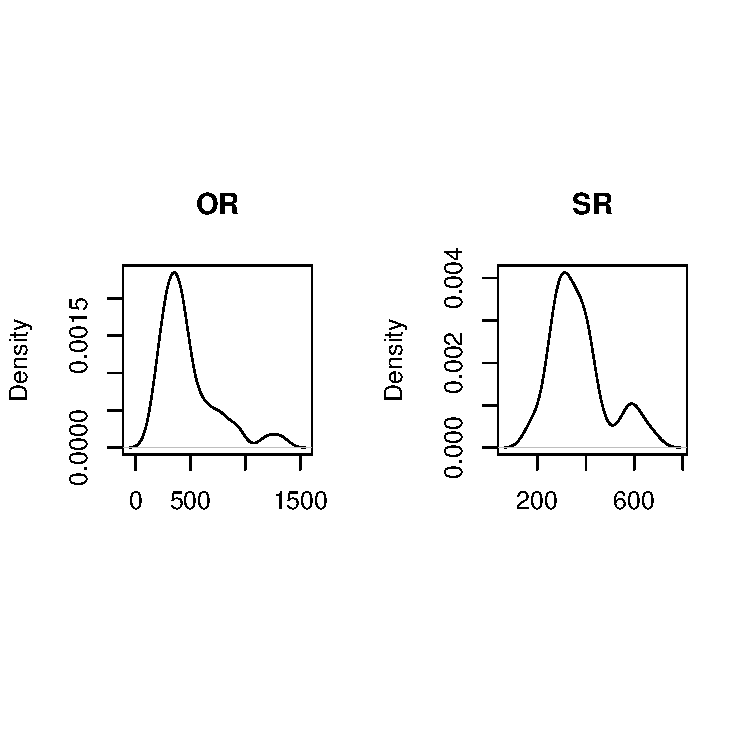
\includegraphics[width=\maxwidth]{figure/unnamed-chunk-80-1} 

\end{knitrout}

The empirical density plots shown above don't seem to show a normal distribution, as assumed in the equation we wrote above:

\begin{equation}
Y \sim Normal(\mu,\sigma)
\end{equation}

If anything, in each condition, the underlying pdf is more like a LogNormal:

\begin{equation}
Y \sim LogNormal(\mu,\sigma)
\end{equation}

Actually, it's even more complicated than that: it seems to be a mixture distribution. See \cite{VasishthMixture2017} for more discussion on this point. 

It is pretty common in psycholinguistics to ignore the normality violation of the modeling assumption! For now, we will also ignore it; later on, we will return to this point. 

Looking at the means by condition, it is clear that object relatives have a longer reading time at the relative clause verb \textit{sent}.

\begin{knitrout}
\definecolor{shadecolor}{rgb}{0.969, 0.969, 0.969}\color{fgcolor}\begin{kframe}
\begin{alltt}
\hlstd{means}\hlkwb{<-}\hlkwd{round}\hlstd{(}\hlkwd{with}\hlstd{(dat,}
                  \hlkwd{tapply}\hlstd{(rawRT,condition,mean)))}
\hlstd{means}
\end{alltt}
\begin{verbatim}
##  objgap subjgap 
##     471     369
\end{verbatim}
\end{kframe}
\end{knitrout}

This is how one could do a t-test with such data, to compare means across (sets of) conditions. 

\begin{knitrout}
\definecolor{shadecolor}{rgb}{0.969, 0.969, 0.969}\color{fgcolor}\begin{kframe}
\begin{alltt}
\hlkwd{t.test}\hlstd{(SR,OR,}\hlkwc{paired}\hlstd{=}\hlnum{TRUE}\hlstd{)}
\end{alltt}
\begin{verbatim}
## 
## 	Paired t-test
## 
## data:  SR and OR
## t = -3.1093, df = 41, p-value = 0.003404
## alternative hypothesis: true difference in means is not equal to 0
## 95 percent confidence interval:
##  -168.72119  -35.85024
## sample estimates:
## mean of the differences 
##               -102.2857
\end{verbatim}
\end{kframe}
\end{knitrout}

This is the one-sample t-test we saw earlier, where we subtract each subject's OR reading time from that subject's SR reading time and get a vector of scores.

\begin{knitrout}
\definecolor{shadecolor}{rgb}{0.969, 0.969, 0.969}\color{fgcolor}\begin{kframe}
\begin{alltt}
\hlkwd{t.test}\hlstd{(SR}\hlopt{-}\hlstd{OR)}
\end{alltt}
\begin{verbatim}
## 
## 	One Sample t-test
## 
## data:  SR - OR
## t = -3.1093, df = 41, p-value = 0.003404
## alternative hypothesis: true mean is not equal to 0
## 95 percent confidence interval:
##  -168.72119  -35.85024
## sample estimates:
## mean of x 
## -102.2857
\end{verbatim}
\end{kframe}
\end{knitrout}

For comparison, the published result in \cite{grodner} is:  t1(1, 41) = 11.9, p $<$ .001. The t1 refers to aggregation over items we did above. The published effect is larger because they deleted some extreme values. On p.\ 268, the authors write:


\begin{quote}
Reading times that differed from the mean of a condition and region by more than 3 SDs were omitted from analyses. This adjustment discarded 1.6\% of the data. 
\end{quote}

It's not clear from this text whether this is on the unaggregated data or the aggregated data. It cannot be on the aggregated data, because then 19 out of 42 data points would be considered extreme in subject relatives:

\begin{knitrout}
\definecolor{shadecolor}{rgb}{0.969, 0.969, 0.969}\color{fgcolor}\begin{kframe}
\begin{alltt}
\hlnum{3}\hlopt{*}\hlkwd{sd}\hlstd{(OR)}
\end{alltt}
\begin{verbatim}
## [1] 779.6772
\end{verbatim}
\begin{alltt}
\hlnum{3}\hlopt{*}\hlkwd{sd}\hlstd{(SR)}
\end{alltt}
\begin{verbatim}
## [1] 353.0165
\end{verbatim}
\begin{alltt}
\hlstd{deletionOR}\hlkwb{<-}\hlkwd{ifelse}\hlstd{(OR}\hlopt{>}\hlnum{3}\hlopt{*}\hlkwd{sd}\hlstd{(OR),}\hlstr{"remove"}\hlstd{,}\hlstr{"keep"}\hlstd{)}
\hlstd{deletionSR}\hlkwb{<-}\hlkwd{ifelse}\hlstd{(SR}\hlopt{>}\hlnum{3}\hlopt{*}\hlkwd{sd}\hlstd{(SR),}\hlstr{"remove"}\hlstd{,}\hlstr{"keep"}\hlstd{)}
\hlkwd{table}\hlstd{(deletionOR)}
\end{alltt}
\begin{verbatim}
## deletionOR
##   keep remove 
##     37      5
\end{verbatim}
\begin{alltt}
\hlkwd{table}\hlstd{(deletionSR)}
\end{alltt}
\begin{verbatim}
## deletionSR
##   keep remove 
##     23     19
\end{verbatim}
\end{kframe}
\end{knitrout}

For now we ignore this discrepancy between the published result and our finding above in the t-test.

Next, we will fit a \textbf{linear model} to these data. First, create a data frame in so-called long format for doing the data analysis.

\begin{knitrout}
\definecolor{shadecolor}{rgb}{0.969, 0.969, 0.969}\color{fgcolor}\begin{kframe}
\begin{alltt}
\hlstd{aggregated_data}\hlkwb{<-}\hlkwd{data.frame}\hlstd{(}
  \hlkwc{subj}\hlstd{=}\hlkwd{rep}\hlstd{(}\hlnum{1}\hlopt{:}\hlnum{42}\hlstd{,}\hlnum{2}\hlstd{),}
  \hlkwc{cond}\hlstd{=}\hlkwd{factor}\hlstd{(}\hlkwd{rep}\hlstd{(}\hlkwd{c}\hlstd{(}\hlstr{"or"}\hlstd{,}\hlstr{"sr"}\hlstd{),}\hlkwc{each}\hlstd{=}\hlnum{42}\hlstd{)),}
              \hlkwc{rt}\hlstd{=}\hlkwd{c}\hlstd{(OR,SR))}
\end{alltt}
\end{kframe}
\end{knitrout}

\begin{knitrout}
\definecolor{shadecolor}{rgb}{0.969, 0.969, 0.969}\color{fgcolor}\begin{kframe}
\begin{alltt}
\hlstd{m0}\hlkwb{<-}\hlkwd{lm}\hlstd{(rt}\hlopt{~}\hlstd{cond,aggregated_data)}
\hlkwd{summary}\hlstd{(m0)}
\end{alltt}
\begin{verbatim}
## 
## Call:
## lm(formula = rt ~ cond, data = aggregated_data)
## 
## Residuals:
##     Min      1Q  Median      3Q     Max 
## -303.36 -116.35  -51.59   49.05  853.26 
## 
## Coefficients:
##             Estimate Std. Error t value Pr(>|t|)    
## (Intercept)   471.36      31.13  15.143   <2e-16 ***
## condsr       -102.29      44.02  -2.324   0.0226 *  
## ---
## Signif. codes:  0 '***' 0.001 '**' 0.01 '*' 0.05 '.' 0.1 ' ' 1
## 
## Residual standard error: 201.7 on 82 degrees of freedom
## Multiple R-squared:  0.06177,	Adjusted R-squared:  0.05033 
## F-statistic: 5.399 on 1 and 82 DF,  p-value: 0.02263
\end{verbatim}
\end{kframe}
\end{knitrout}

This linear model fits the same model as the  \textbf{two-sample} t-test we saw earlier:

\begin{knitrout}
\definecolor{shadecolor}{rgb}{0.969, 0.969, 0.969}\color{fgcolor}\begin{kframe}
\begin{alltt}
\hlkwd{t.test}\hlstd{(SR,OR,}\hlkwc{paired}\hlstd{=}\hlnum{FALSE}\hlstd{)}
\end{alltt}
\begin{verbatim}
## 
## 	Welch Two Sample t-test
## 
## data:  SR and OR
## t = -2.3235, df = 57.132, p-value = 0.02373
## alternative hypothesis: true difference in means is not equal to 0
## 95 percent confidence interval:
##  -190.43245  -14.13898
## sample estimates:
## mean of x mean of y 
##  369.0744  471.3601
\end{verbatim}
\end{kframe}
\end{knitrout}

Notice that the t-value is the same in the t-test and the linear model.

Since the two-sample t-test is the wrong model (this is paired data), the linear model is obviously also an incorrect model for the aggregated data. We don't want to treat the data as unpaired if they are paired. We will soon fit the correct model. For now, let's focus on understanding what the linear model gives us.

\subsubsection{Unpacking the linear model output}

First, look at the coefficients, which define the \textbf{intercept} and \textbf{slope} of the fitted line respectively:

\begin{knitrout}
\definecolor{shadecolor}{rgb}{0.969, 0.969, 0.969}\color{fgcolor}\begin{kframe}
\begin{alltt}
\hlcom{## coefficients:}
\hlkwd{coef}\hlstd{(m0)}
\end{alltt}
\begin{verbatim}
## (Intercept)      condsr 
##    471.3601   -102.2857
\end{verbatim}
\end{kframe}
\end{knitrout}

Compare these coefficients with the means we computed above.

\begin{knitrout}
\definecolor{shadecolor}{rgb}{0.969, 0.969, 0.969}\color{fgcolor}\begin{kframe}
\begin{alltt}
\hlstd{means}
\end{alltt}
\begin{verbatim}
##  objgap subjgap 
##     471     369
\end{verbatim}
\end{kframe}
\end{knitrout}

The mean for SRs is 369 ms, and the mean for ORs is 369+102=471.

The fitted linear model implies two generative processes for the two conditions:

ORs:

\begin{equation}
y_{obj} =  471 + \varepsilon \hbox{ where } \varepsilon \sim Normal(0,201)
\end{equation}

SRs:

\begin{equation}
y_{subj} =  471 - 102 +  \varepsilon \hbox{ where } \varepsilon \sim Normal(0,201)
\end{equation}

This is encoded in the data frame by coding rows containing object relatives as 0's and rows containing subject relatives as 1's. This is called \textbf{treatment contrast coding}. We return to this below.

One assumption the model makes is that the $\varepsilon$, which are called the residuals, are normally distributed: $\varepsilon \sim Normal(0,\sigma)$. We can check whether this assumption is met by examining the distribution of the residuals.
We can extract the residuals:

\begin{knitrout}
\definecolor{shadecolor}{rgb}{0.969, 0.969, 0.969}\color{fgcolor}\begin{kframe}
\begin{alltt}
\hlcom{## residuals:}
\hlstd{res.m0}\hlkwb{<-}\hlkwd{residuals}\hlstd{(m0)}
\end{alltt}
\end{kframe}
\end{knitrout}


and plot them by comparing them to a standard normal distribution. If the residuals are approximately normal, you should see the data points along a straight line angled at 45 degrees. This is clearly not true in our data.

\begin{figure}[!htbp]
\centering
\begin{knitrout}
\definecolor{shadecolor}{rgb}{0.969, 0.969, 0.969}\color{fgcolor}\begin{kframe}
\begin{alltt}
\hlkwd{library}\hlstd{(car)}
\hlkwd{qqPlot}\hlstd{(res.m0)}
\end{alltt}
\end{kframe}
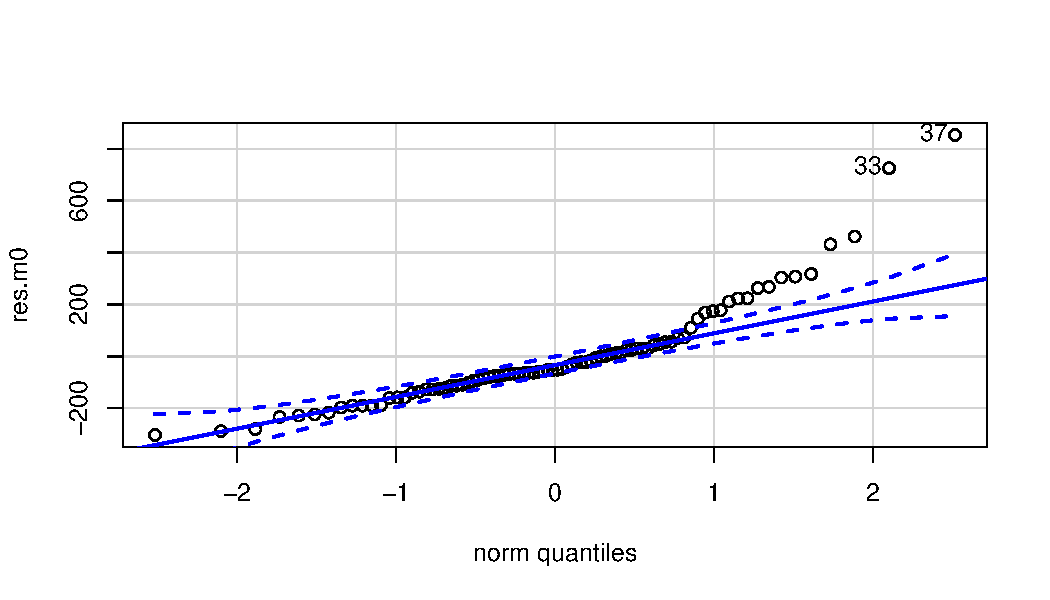
\includegraphics[width=\maxwidth]{figure/unnamed-chunk-91-1} 
\begin{kframe}\begin{verbatim}
## [1] 37 33
\end{verbatim}
\end{kframe}
\end{knitrout}
\caption{Residuals of the model m0.}
\label{fig:residuals}
\end{figure}

A straightforward solution we will consider later is a log-transform of the reading times.

\begin{knitrout}
\definecolor{shadecolor}{rgb}{0.969, 0.969, 0.969}\color{fgcolor}\begin{kframe}
\begin{alltt}
\hlstd{m0log}\hlkwb{<-}\hlkwd{lm}\hlstd{(}\hlkwd{log}\hlstd{(rt)}\hlopt{~}\hlstd{cond,aggregated_data)}
\hlkwd{summary}\hlstd{(m0log)}
\end{alltt}
\begin{verbatim}
## 
## Call:
## lm(formula = log(rt) ~ cond, data = aggregated_data)
## 
## Residuals:
##      Min       1Q   Median       3Q      Max 
## -0.90909 -0.23721 -0.02533  0.17128  1.15583 
## 
## Coefficients:
##             Estimate Std. Error t value Pr(>|t|)    
## (Intercept)  6.03305    0.06278  96.098   <2e-16 ***
## condsr      -0.16858    0.08878  -1.899   0.0611 .  
## ---
## Signif. codes:  0 '***' 0.001 '**' 0.01 '*' 0.05 '.' 0.1 ' ' 1
## 
## Residual standard error: 0.4069 on 82 degrees of freedom
## Multiple R-squared:  0.04211,	Adjusted R-squared:  0.03043 
## F-statistic: 3.605 on 1 and 82 DF,  p-value: 0.06111
\end{verbatim}
\end{kframe}
\end{knitrout}

Notice two things that changed. First, our significant effect is no longer significant.
This is because the effect we found above was driven by a few extreme values. Of course, if we had done the analysis correctly (treating the data as paired, as it should be), we would have obtained a significant effect:

\begin{knitrout}
\definecolor{shadecolor}{rgb}{0.969, 0.969, 0.969}\color{fgcolor}\begin{kframe}
\begin{alltt}
\hlkwd{t.test}\hlstd{(}\hlkwd{log}\hlstd{(OR)}\hlopt{-}\hlkwd{log}\hlstd{(SR))}
\end{alltt}
\begin{verbatim}
## 
## 	One Sample t-test
## 
## data:  log(OR) - log(SR)
## t = 2.9227, df = 41, p-value = 0.005624
## alternative hypothesis: true mean is not equal to 0
## 95 percent confidence interval:
##  0.05209544 0.28506346
## sample estimates:
## mean of x 
## 0.1685795
\end{verbatim}
\end{kframe}
\end{knitrout}




Second, the residuals are now much more normal---model assumptions are met much better than when we analyzed the raw reading times.

\begin{knitrout}
\definecolor{shadecolor}{rgb}{0.969, 0.969, 0.969}\color{fgcolor}\begin{kframe}
\begin{alltt}
\hlkwd{qqPlot}\hlstd{(}\hlkwd{residuals}\hlstd{(m0log))}
\end{alltt}
\end{kframe}
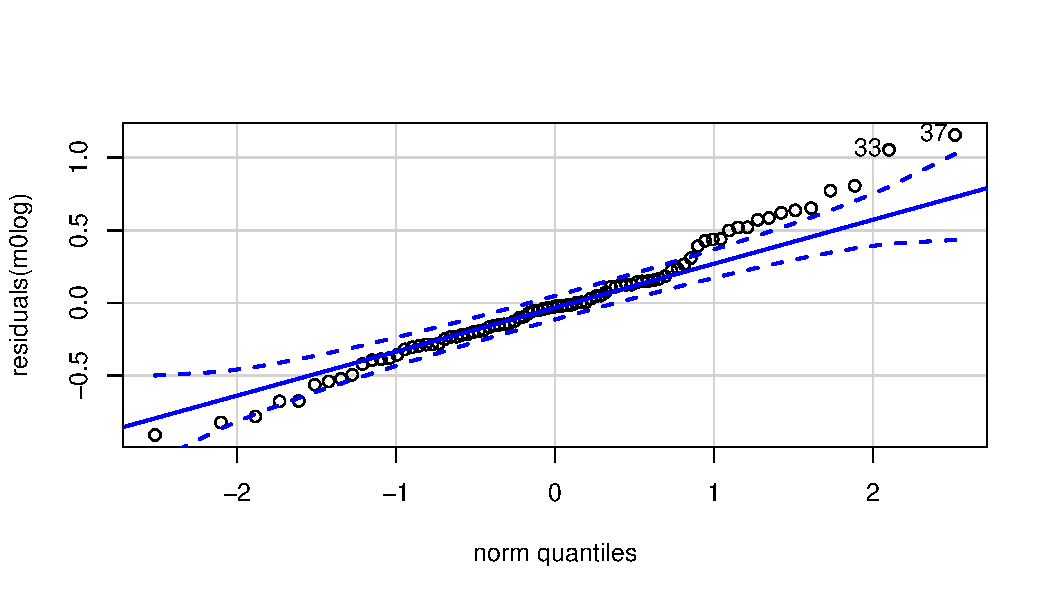
\includegraphics[width=\maxwidth]{figure/unnamed-chunk-94-1} 
\begin{kframe}\begin{verbatim}
## [1] 37 33
\end{verbatim}
\end{kframe}
\end{knitrout}

Subjects 33 and 37 seem to show interestingly extreme behavior; a topic we will return to later in the next chapter.

\subsubsection{How the coefficient estimates are computed}

Underlyingly, R uses a design matrix or model matrix, which is being used by R to estimate the coefficients:

\begin{knitrout}
\definecolor{shadecolor}{rgb}{0.969, 0.969, 0.969}\color{fgcolor}\begin{kframe}
\begin{alltt}
\hlcom{##}
\hlkwd{head}\hlstd{(}\hlkwd{model.matrix}\hlstd{(m0),}\hlkwc{n}\hlstd{=}\hlnum{7}\hlstd{)}
\end{alltt}
\begin{verbatim}
##   (Intercept) condsr
## 1           1      0
## 2           1      0
## 3           1      0
## 4           1      0
## 5           1      0
## 6           1      0
## 7           1      0
\end{verbatim}
\end{kframe}
\end{knitrout}

It is very useful to understand a little bit about what these parts of the linear model are.
Our linear model equation for the relative clause model m0 above is a system of equations. The single equation:

\begin{equation} \label{eq1a}
Y_i = \beta_{0} + \beta_{1}X_i + \epsilon_i 
\end{equation}

\noindent
can be expanded to:

\begin{equation} \label{matrixeq1}
 \begin{array}{ccccccc}
Y_1    & = & \beta_0 & + & X_1 \beta_1 & + & \epsilon_1 \\
Y_2    & = & \beta_0 & + & X_2 \beta_1 & + & \epsilon_2 \\
Y_3    & = & \beta_0  & + & X_3 \beta_1 & + & \epsilon_3 \\
Y_4    & = & \beta_0 & + & X_4 \beta_1 & + & \epsilon_4 \\
\vdots &   & \vdots  &   & \vdots      &   & \vdots  \\
Y_{84}    & = & \beta_0 & + & X_{84} \beta_1 & + & \epsilon_{84} \\
\end{array} 
\end{equation}

The total number of rows $n$ here is 42*2=84 in the Grodner and Gibson data. This is because in the aggregated data we created above, each subject delivers two data points, one for SRs and one for ORs, and there are 42 subjects.

This system of linear equations can be restated in compact matrix form:

\begin{equation}
\mathbf{Y} = \mathbf{X} \mathbf{\beta} + \mathbf{\epsilon}
\end{equation}



\noindent
where

\textbf{Vector of responses}:

\begin{equation} \label{matrixsum}
\mathbf{Y} = \left( \begin{array}{c}
Y_1 \\
Y_2 \\
Y_3 \\
Y_4 \\
\vdots \\
Y_n \\
\end{array} \right)
\end{equation}

\textbf{The design matrix (in R this is called the model matrix)}:

\begin{equation} \label{matrixsum}
\mathbf{X} = \left( \begin{array}{cc}
1 & X_1 \\
1 & X_2 \\
1 & X_3 \\
1 & X_4 \\
\vdots & \vdots \\
1 & X_n \\
\end{array} \right)
\end{equation}

\textbf{Vector of coefficient parameters to be estimated}:

\begin{equation} \label{matrixsum}
\mathbf{\beta} = \left( \begin{array}{c}
\beta_0 \\
\beta_1 \\
\end{array} \right)
\end{equation}

and 

\textbf{Vector of error terms (residuals)}:

\begin{equation} \label{matrixsum}
\mathbf{\epsilon} = \left( \begin{array}{c}
\epsilon_1 \\
\epsilon_2 \\
\epsilon_3 \\
\epsilon_4 \\
\vdots \\
\epsilon_n \\
\end{array} \right)
\end{equation}

We could write the whole equation as:

\begin{equation} \label{matrixsum}
\left( \begin{array}{c}
Y_1 \\
Y_2 \\
Y_3 \\
Y_4 \\
\vdots \\
Y_n \\
\end{array} \right)
=
\left( \begin{array}{cc}
1 & X_1 \\
1 & X_2 \\
1 & X_3 \\
1 & X_4 \\
\vdots & \vdots \\
1 & X_n \\
\end{array} \right) 
\times 
\left( \begin{array}{c}
\beta_1 \\
\beta_2 \\
\end{array} \right)
+
\left( \begin{array}{c}
\epsilon_1 \\
\epsilon_2 \\
\epsilon_3 \\
\epsilon_4 \\
\vdots \\
\epsilon_n \\
\end{array} \right)
\end{equation}

Our principal goal when we fit a linear model is to find estimates of the parameters $\beta_0$ and $\beta_1$, the intercept and slope respectively; we will call the estimates from the data $\hat{\beta}_0$ and $\hat{\beta}_1$, in order to distinguish them from the unknown population parameters $\beta_0$ and $\beta_1$. This can be done by ``solving'' for the beta's using linear algebra. X is the model matrix, and X$'$ is the transpose of the model matrix. Y is the vector of dependent variables.

\begin{equation}
\beta=(X'X)^{-1} X'Y 
\end{equation}

You do not need to know how the above equation comes about; all you need to know is that given X, and Y, we can estimate the parameters.
In case you are interested in more details, please see my lecture notes on Linear Modeling: https://osf.io/ces89/.


Let's focus now on the vector $X_1,\dots,X_n$ in the model matrix. The first 42 values are 0 and the last 42 values are 1. This is because of the treatment contrast coding, which we examine in more detail next.

\subsubsection{Contrast coding}

Look at how each level of the relative clause conditions is converted into a numeric value:

\begin{knitrout}
\definecolor{shadecolor}{rgb}{0.969, 0.969, 0.969}\color{fgcolor}\begin{kframe}
\begin{alltt}
\hlkwd{contrasts}\hlstd{(aggregated_data}\hlopt{$}\hlstd{cond)}
\end{alltt}
\begin{verbatim}
##    sr
## or  0
## sr  1
\end{verbatim}
\end{kframe}
\end{knitrout}


The above contrast coding says the following: code object relatives as 0 and subject relatives as 1. 
Alphabetic order of the factor levels determines which level gets the 0 value. You can switch the order of the coding manually by doing the following:

\begin{knitrout}
\definecolor{shadecolor}{rgb}{0.969, 0.969, 0.969}\color{fgcolor}\begin{kframe}
\begin{alltt}
\hlstd{aggregated_data}\hlopt{$}\hlstd{cond}\hlkwb{<-}\hlkwd{factor}\hlstd{(aggregated_data}\hlopt{$}\hlstd{cond,}\hlkwc{levels}\hlstd{=}\hlkwd{c}\hlstd{(}\hlstr{"sr"}\hlstd{,}\hlstr{"or"}\hlstd{))}
\end{alltt}
\end{kframe}
\end{knitrout}

Another way, which we will use in future, is to just create a new vector of 0,1 values using ifelse:

\begin{knitrout}
\definecolor{shadecolor}{rgb}{0.969, 0.969, 0.969}\color{fgcolor}\begin{kframe}
\begin{alltt}
\hlstd{aggregated_data}\hlopt{$}\hlstd{c_trtmt}\hlkwb{<-}\hlkwd{ifelse}\hlstd{(aggregated_data}\hlopt{$}\hlstd{cond}\hlopt{==}\hlstr{"sr"}\hlstd{,}\hlnum{0}\hlstd{,}\hlnum{1}\hlstd{)}
\end{alltt}
\end{kframe}
\end{knitrout}

As mentioned above, this kind of contrast is called treatment contrast coding.  

An alternative contrast coding is called sum contrasts: under this coding, object relatives are coded as 1 and subject relatives as -1 (the coding is arbitrary; we could have had it the other way around).

\begin{knitrout}
\definecolor{shadecolor}{rgb}{0.969, 0.969, 0.969}\color{fgcolor}\begin{kframe}
\begin{alltt}
\hlkwd{contrasts}\hlstd{(aggregated_data}\hlopt{$}\hlstd{cond)}\hlkwb{<-}\hlkwd{contr.sum}\hlstd{(}\hlnum{2}\hlstd{)}
\hlkwd{contrasts}\hlstd{(aggregated_data}\hlopt{$}\hlstd{cond)}
\end{alltt}
\begin{verbatim}
##    [,1]
## sr    1
## or   -1
\end{verbatim}
\end{kframe}
\end{knitrout}

We can also define such a contrast coding by creating a new vector:

\begin{knitrout}
\definecolor{shadecolor}{rgb}{0.969, 0.969, 0.969}\color{fgcolor}\begin{kframe}
\begin{alltt}
\hlstd{aggregated_data}\hlopt{$}\hlstd{c_sum}\hlkwb{<-}\hlkwd{ifelse}\hlstd{(aggregated_data}\hlopt{$}\hlstd{cond}\hlopt{==}\hlstr{"sr"}\hlstd{,}\hlopt{-}\hlnum{1}\hlstd{,}\hlnum{1}\hlstd{)}
\end{alltt}
\end{kframe}
\end{knitrout}


Now, the model looks like this:

\begin{knitrout}
\definecolor{shadecolor}{rgb}{0.969, 0.969, 0.969}\color{fgcolor}\begin{kframe}
\begin{alltt}
\hlstd{m2}\hlkwb{<-}\hlkwd{lm}\hlstd{(rt}\hlopt{~}\hlstd{c_sum,aggregated_data)}
\hlkwd{summary}\hlstd{(m2)}
\end{alltt}
\begin{verbatim}
## 
## Call:
## lm(formula = rt ~ c_sum, data = aggregated_data)
## 
## Residuals:
##     Min      1Q  Median      3Q     Max 
## -303.36 -116.35  -51.59   49.05  853.26 
## 
## Coefficients:
##             Estimate Std. Error t value Pr(>|t|)    
## (Intercept)   420.22      22.01  19.092   <2e-16 ***
## c_sum          51.14      22.01   2.324   0.0226 *  
## ---
## Signif. codes:  0 '***' 0.001 '**' 0.01 '*' 0.05 '.' 0.1 ' ' 1
## 
## Residual standard error: 201.7 on 82 degrees of freedom
## Multiple R-squared:  0.06177,	Adjusted R-squared:  0.05033 
## F-statistic: 5.399 on 1 and 82 DF,  p-value: 0.02263
\end{verbatim}
\end{kframe}
\end{knitrout}

The intercept is now the grand mean:

\begin{knitrout}
\definecolor{shadecolor}{rgb}{0.969, 0.969, 0.969}\color{fgcolor}\begin{kframe}
\begin{alltt}
\hlkwd{round}\hlstd{(}\hlkwd{mean}\hlstd{(aggregated_data}\hlopt{$}\hlstd{rt),}\hlnum{2}\hlstd{)}
\end{alltt}
\begin{verbatim}
## [1] 420.22
\end{verbatim}
\end{kframe}
\end{knitrout}

The difference between the reading times can be computed from the slope as follows:

\begin{knitrout}
\definecolor{shadecolor}{rgb}{0.969, 0.969, 0.969}\color{fgcolor}\begin{kframe}
\begin{alltt}
\hlstd{(ORmeans}\hlkwb{<-}\hlnum{420.21726}\hlopt{+}\hlnum{51.14286}\hlstd{)}
\end{alltt}
\begin{verbatim}
## [1] 471.3601
\end{verbatim}
\begin{alltt}
\hlstd{(SRmeans}\hlkwb{<-}\hlnum{420.21726}\hlopt{-}\hlnum{51.14286}\hlstd{)}
\end{alltt}
\begin{verbatim}
## [1] 369.0744
\end{verbatim}
\begin{alltt}
\hlcom{## difference in means:}
\hlstd{SRmeans}\hlopt{-}\hlstd{ORmeans}
\end{alltt}
\begin{verbatim}
## [1] -102.2857
\end{verbatim}
\end{kframe}
\end{knitrout}

As mentioned above, in future, we will be using not the treatment contrast coding but this sum contrast coding.

\subsection{True discovery rate (power)}

Even before we had collected the data, we should have done a power analysis. We should make sure that we have adequate power before we run the experiment, otherwise the logic of NHST doesn't work, due to Type M and S errors. We can check prospective power \textit{for a future study} as follows:

In the published paper, the difference between object and subject relative reading times was 65 ms. If that's the true value of the effect, then we could compute power as follows, assuming a standard deviation of 213. This sd is estimated from the Grodner and Gibson data as follows:

The one-sample t-test gave us a t-value of -3.1, and the difference in means is -102. Sample size is 42. We know from the t-test that:

\begin{equation}
t= -3.1=\frac{-102}{s/\sqrt{42}}
\end{equation}

So just solve for s (exercise). The answer is approximately 213. 

\begin{knitrout}
\definecolor{shadecolor}{rgb}{0.969, 0.969, 0.969}\color{fgcolor}\begin{kframe}
\begin{alltt}
\hlkwd{power.t.test}\hlstd{(}\hlkwc{d}\hlstd{=}\hlnum{65}\hlstd{,}\hlkwc{sd}\hlstd{=}\hlnum{213}\hlstd{,}\hlkwc{type}\hlstd{=}\hlstr{"one.sample"}\hlstd{,}\hlkwc{n}\hlstd{=}\hlnum{42}\hlstd{)}
\end{alltt}
\begin{verbatim}
## 
##      One-sample t test power calculation 
## 
##               n = 42
##           delta = 65
##              sd = 213
##       sig.level = 0.05
##           power = 0.4885604
##     alternative = two.sided
\end{verbatim}
\end{kframe}
\end{knitrout}

The above is an analytical solution that R provides, based on closed-form formulas that you can find in statistics textbooks.

50\% power is too low. How many subjects should we have collected data from if we wanted 80\% power?

\begin{knitrout}
\definecolor{shadecolor}{rgb}{0.969, 0.969, 0.969}\color{fgcolor}\begin{kframe}
\begin{alltt}
\hlkwd{power.t.test}\hlstd{(}\hlkwc{d}\hlstd{=}\hlnum{65}\hlstd{,}\hlkwc{sd}\hlstd{=}\hlnum{213}\hlstd{,}\hlkwc{power}\hlstd{=}\hlnum{0.80}\hlstd{,}\hlkwc{type}\hlstd{=}\hlstr{"one.sample"}\hlstd{)}
\end{alltt}
\begin{verbatim}
## 
##      One-sample t test power calculation 
## 
##               n = 86.22349
##           delta = 65
##              sd = 213
##       sig.level = 0.05
##           power = 0.8
##     alternative = two.sided
\end{verbatim}
\end{kframe}
\end{knitrout}

The answer is 87 subjects at a minimum. 

In such a situation, I would also ask: suppose the true effect is not 65 ms but 30 ms. We know that under low power conditions, any significant effect we find is guaranteed to be an overestimate. So Grodner and Gibson's estimate is probably biased upwards (Type M error) if their power is this low. 

How many subjects would we need to obtain 80\% power, if the true effect was as low as 30 ms? The answer may shock you:

\begin{knitrout}
\definecolor{shadecolor}{rgb}{0.969, 0.969, 0.969}\color{fgcolor}\begin{kframe}
\begin{alltt}
\hlkwd{power.t.test}\hlstd{(}\hlkwc{d}\hlstd{=}\hlnum{30}\hlstd{,}\hlkwc{sd}\hlstd{=}\hlnum{213}\hlstd{,}\hlkwc{power}\hlstd{=}\hlnum{0.80}\hlstd{,}\hlkwc{type}\hlstd{=}\hlstr{"one.sample"}\hlstd{)}
\end{alltt}
\begin{verbatim}
## 
##      One-sample t test power calculation 
## 
##               n = 397.587
##           delta = 30
##              sd = 213
##       sig.level = 0.05
##           power = 0.8
##     alternative = two.sided
\end{verbatim}
\end{kframe}
\end{knitrout}

The reality is that small effects in areas like sentence processing are quite common. All the big and robust effects have already been found.
Studies tend to be heavily underpowered, leading to exaggerated estimates getting published. See my papers \cite{VasishthMertzenJaegerGelman2018,JaegerEngelmannVasishth2017} for extended dicussions about this point in the context of sentence processing.

When doing such power calculations, one can also compute power curve for different effect sizes, given a sample size:

\begin{knitrout}
\definecolor{shadecolor}{rgb}{0.969, 0.969, 0.969}\color{fgcolor}\begin{kframe}
\begin{alltt}
\hlstd{effect}\hlkwb{<-}\hlkwd{seq}\hlstd{(}\hlnum{10}\hlstd{,}\hlnum{65}\hlstd{,}\hlkwc{by}\hlstd{=}\hlnum{0.1}\hlstd{)}
\hlstd{pow}\hlkwb{<-}\hlkwd{rep}\hlstd{(}\hlnum{NA}\hlstd{,}\hlkwd{length}\hlstd{(effect))}

\hlkwa{for}\hlstd{(i} \hlkwa{in} \hlnum{1}\hlopt{:}\hlkwd{length}\hlstd{(effect))\{}
\hlstd{pow[i]}\hlkwb{<-}\hlkwd{power.t.test}\hlstd{(}\hlkwc{d}\hlstd{=effect[i],}\hlkwc{sd}\hlstd{=}\hlnum{213}\hlstd{,}\hlkwc{n}\hlstd{=}\hlnum{42}\hlstd{,}
             \hlkwc{type}\hlstd{=}\hlstr{"one.sample"}\hlstd{)}\hlopt{$}\hlstd{power}
\hlstd{\}}
\hlkwd{plot}\hlstd{(effect,pow,}\hlkwc{type}\hlstd{=}\hlstr{"l"}\hlstd{,}
     \hlkwc{main}\hlstd{=}\hlstr{"power curve (n=42,sigma=213)"}\hlstd{,}
     \hlkwc{xlab}\hlstd{=}\hlstr{"effect (ms)"}\hlstd{,}\hlkwc{ylab}\hlstd{=}\hlstr{"power"}\hlstd{)}
\end{alltt}
\end{kframe}
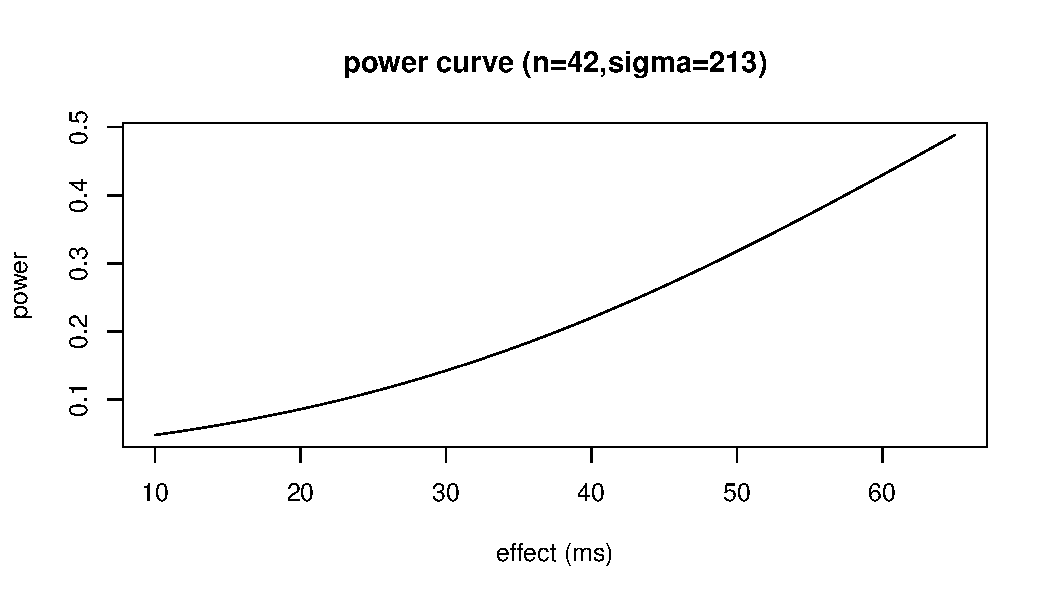
\includegraphics[width=\maxwidth]{figure/unnamed-chunk-107-1} 

\end{knitrout}

This concludes our introduction to linear models when we have an experiment with a factorial design (here, two conditions).
Next, we consider the case where we have a continuous predictor.


\section{A linear model with a continuous predictor}

In our relative clause example, the predictor is categorial. What about when we have continuous predictors. An example is  instructors' beauty levels measured on a continuous scale as predictors of their teaching evaluations? Beauty levels are centered; this means that a beauty level of 0 means average beauty level. This is a data set from a paper by 
Hamermesh and Parker
(Beauty in the Classroom: Instructors' Pulchritude and Putative Pedagogical Productivity," Economics of Education Review, August 2005). I got the data from \cite{gelmanhill07}. 




\begin{knitrout}
\definecolor{shadecolor}{rgb}{0.969, 0.969, 0.969}\color{fgcolor}\begin{kframe}
\begin{alltt}
\hlcom{## Example with a continuous predictor:}

\hlcom{## teacher's evaluations as a function of their beauty score:}
\hlstd{bdata} \hlkwb{<-} \hlkwd{read.table}\hlstd{(}\hlstr{"data/beauty.txt"}\hlstd{,}\hlkwc{header}\hlstd{=}\hlnum{TRUE}\hlstd{)}
\hlkwd{head}\hlstd{(bdata)}
\end{alltt}
\begin{verbatim}
##       beauty evaluation
## 1  0.2015666        4.3
## 2 -0.8260813        4.5
## 3 -0.6603327        3.7
## 4 -0.7663125        4.3
## 5  1.4214450        4.4
## 6  0.5002196        4.2
\end{verbatim}
\end{kframe}
\end{knitrout}

Let's first plot the data first:

\begin{knitrout}
\definecolor{shadecolor}{rgb}{0.969, 0.969, 0.969}\color{fgcolor}\begin{kframe}
\begin{alltt}
\hlkwd{plot}\hlstd{(evaluation}\hlopt{~}\hlstd{beauty,bdata)}
\end{alltt}
\end{kframe}
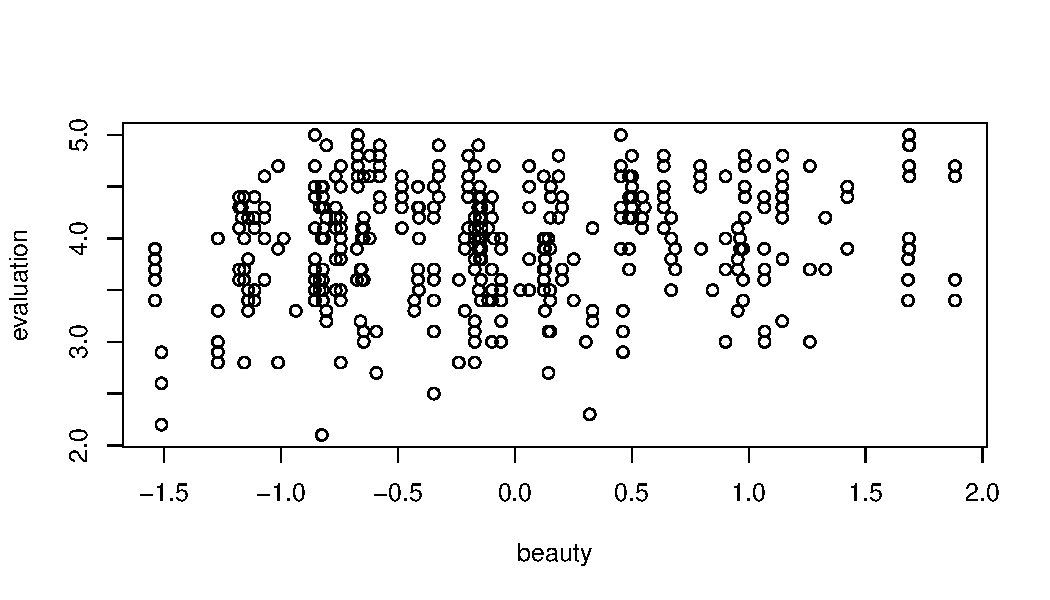
\includegraphics[width=\maxwidth]{figure/unnamed-chunk-109-1} 

\end{knitrout}


\begin{knitrout}
\definecolor{shadecolor}{rgb}{0.969, 0.969, 0.969}\color{fgcolor}\begin{kframe}
\begin{alltt}
\hlstd{m3}\hlkwb{<-}\hlkwd{lm}\hlstd{(evaluation}\hlopt{~}\hlstd{beauty,bdata)}
\end{alltt}
\end{kframe}
\end{knitrout}

\begin{knitrout}
\definecolor{shadecolor}{rgb}{0.969, 0.969, 0.969}\color{fgcolor}\begin{kframe}
\begin{alltt}
\hlkwd{summary}\hlstd{(m3)}
\end{alltt}
\begin{verbatim}
## 
## Call:
## lm(formula = evaluation ~ beauty, data = bdata)
## 
## Residuals:
##      Min       1Q   Median       3Q      Max 
## -1.80015 -0.36304  0.07254  0.40207  1.10373 
## 
## Coefficients:
##             Estimate Std. Error t value Pr(>|t|)    
## (Intercept)  4.01002    0.02551 157.205  < 2e-16 ***
## beauty       0.13300    0.03218   4.133 4.25e-05 ***
## ---
## Signif. codes:  0 '***' 0.001 '**' 0.01 '*' 0.05 '.' 0.1 ' ' 1
## 
## Residual standard error: 0.5455 on 461 degrees of freedom
## Multiple R-squared:  0.03574,	Adjusted R-squared:  0.03364 
## F-statistic: 17.08 on 1 and 461 DF,  p-value: 4.247e-05
\end{verbatim}
\end{kframe}
\end{knitrout}

The intercept tells you the estimated mean teaching evaluation when the beauty level (the predictor) has value 0---which is the average ``beauty'' level among these professors. The slope tells you the estimated increase in teaching evaluation when beauty level is increased by 1 unit.

The residuals are roughly normal. Two influential values are marked. You should check what happens if you remove them.

\begin{knitrout}
\definecolor{shadecolor}{rgb}{0.969, 0.969, 0.969}\color{fgcolor}\begin{kframe}
\begin{alltt}
\hlkwd{qqPlot}\hlstd{(}\hlkwd{residuals}\hlstd{(m3))}
\end{alltt}
\end{kframe}
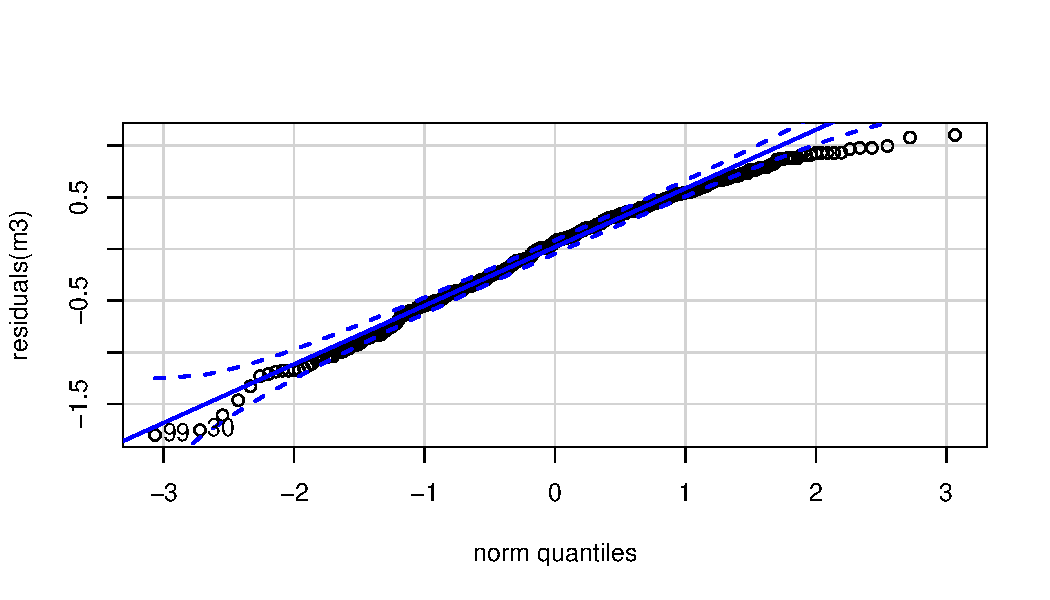
\includegraphics[width=\maxwidth]{figure/unnamed-chunk-112-1} 
\begin{kframe}\begin{verbatim}
## [1] 99 30
\end{verbatim}
\end{kframe}
\end{knitrout}

\subsection{Does beauty level affect evaluation?}

If you look at the p-value in model m3 above, it is clear that we can reject the null hypothesis that beauty level doesn't affect evaluation. But this doesn't mean the effect is real, and it doesn't mean there is a causal link between beauty and evaluations (there could be, it just isn't necessarily so). For one thing, the plot of evaluation against beauty looks very noisy: the points are widely spread out. 

And if power is low, the significant estimate is guaranteed to be exaggerated. Suppose the true effect were half of 0.133. Power would be remarkably low. Let's compute power for this scenario.

I got the sd in the calculation below by looking at the SE of the effect of beauty. $SE=0.03218=s/\sqrt{461}$. So, s=0.69.

\begin{knitrout}
\definecolor{shadecolor}{rgb}{0.969, 0.969, 0.969}\color{fgcolor}\begin{kframe}
\begin{alltt}
\hlkwd{power.t.test}\hlstd{(}\hlkwc{d}\hlstd{=}\hlnum{0.133}\hlopt{/}\hlnum{2}\hlstd{,}\hlkwc{sd}\hlstd{=}\hlnum{0.69}\hlstd{,}\hlkwc{n}\hlstd{=}\hlnum{461}\hlstd{,}\hlkwc{type}\hlstd{=}\hlstr{"two.sample"}\hlstd{)}
\end{alltt}
\begin{verbatim}
## 
##      Two-sample t test power calculation 
## 
##               n = 461
##           delta = 0.0665
##              sd = 0.69
##       sig.level = 0.05
##           power = 0.3091445
##     alternative = two.sided
## 
## NOTE: n is number in *each* group
\end{verbatim}
\end{kframe}
\end{knitrout}

Again, in a potentially low-power situation, we should not trust significant effects. In any case, whether the observed effect of 0.133 has any theoretical relevance would have to worked out through domain expertise. What does a unit increase in beauty mean? Is it even percievable? Does an increase of 0.133  for a unit increase of beauty mean anything important from the perspective of teaching evaluation (I would say no). These kinds of questions should be considered when evaluating an effect; just looking at the p-value is not enough.



\section{Using fake-data simulation to understand a model}

One effective way to understand how well your model represents the phenomenon we are modeling is by fake data simulation.

The beauty model expresses how we think the evaluations were generated. Of course there are other determinants of teaching quality than beauty, so it's not a realistic model. But what data would the model generate under repeated sampling? We can find this out.

First, we define a function that generates fake data, using estimates from our fitted model above. The sample size is as in the beauty data.

\begin{knitrout}
\definecolor{shadecolor}{rgb}{0.969, 0.969, 0.969}\color{fgcolor}\begin{kframe}
\begin{alltt}
\hlstd{gen_fake}\hlkwb{<-}\hlkwa{function}\hlstd{(}\hlkwc{n}\hlstd{=}\hlnum{463}\hlstd{,}\hlkwc{intercept}\hlstd{=}\hlnum{4}\hlstd{,}
                   \hlkwc{slope}\hlstd{=}\hlnum{0.133}\hlstd{,}
         \hlkwc{predictor}\hlstd{=bdata}\hlopt{$}\hlstd{beauty,}
         \hlkwc{sigma}\hlstd{=}\hlnum{0.69}\hlstd{)\{}
  \hlstd{eval}\hlkwb{<-}\hlstd{intercept}\hlopt{+}\hlstd{slope}\hlopt{*}\hlstd{predictor}\hlopt{+}\hlkwd{rnorm}\hlstd{(n,}\hlkwc{mean}\hlstd{=}\hlnum{0}\hlstd{,}\hlkwc{sd}\hlstd{=}\hlnum{0.69}\hlstd{)}
  \hlstd{fakedat}\hlkwb{<-}\hlkwd{data.frame}\hlstd{(}\hlkwc{eval}\hlstd{=eval,}\hlkwc{beauty}\hlstd{=predictor)}
  \hlstd{fakedat}
  \hlstd{\}}
\end{alltt}
\end{kframe}
\end{knitrout}

Then, we generate fake data 10000 times, and save the intercept and slope estimates, and the p-value for the effect of beauty.

\begin{knitrout}
\definecolor{shadecolor}{rgb}{0.969, 0.969, 0.969}\color{fgcolor}\begin{kframe}
\begin{alltt}
\hlstd{nsim}\hlkwb{<-}\hlnum{10000}
\hlstd{savecoef}\hlkwb{<-}\hlkwd{matrix}\hlstd{(}\hlkwd{rep}\hlstd{(}\hlnum{NA}\hlstd{,nsim}\hlopt{*}\hlnum{2}\hlstd{),}\hlkwc{ncol}\hlstd{=}\hlnum{2}\hlstd{)}
\hlstd{pvals}\hlkwb{<-}\hlkwd{rep}\hlstd{(}\hlnum{NA}\hlstd{,nsim)}
\hlcom{#op<-par(mfrow=c(4,5),pty="s")}
\hlkwa{for}\hlstd{(i} \hlkwa{in} \hlnum{1}\hlopt{:}\hlstd{nsim)\{}
  \hlstd{fakedat}\hlkwb{<-}\hlkwd{gen_fake}\hlstd{()}
  \hlstd{m}\hlkwb{<-}\hlkwd{lm}\hlstd{(eval}\hlopt{~}\hlstd{beauty,fakedat)}
 \hlcom{# plot(fakedat[,2],fakedat[,1],}
  \hlcom{#     xlab="beauty",ylab="eval")}
  \hlcom{#abline(m$coef,col="red")}
  \hlstd{savecoef[i,]}\hlkwb{<-}\hlstd{m}\hlopt{$}\hlstd{coef}
  \hlstd{pvals[i]}\hlkwb{<-}\hlkwd{summary}\hlstd{(m)}\hlopt{$}\hlstd{coefficient[}\hlnum{2}\hlstd{,}\hlnum{4}\hlstd{]}
\hlstd{\}}
\end{alltt}
\end{kframe}
\end{knitrout}

Now, we can ask some interesting questions:

\begin{enumerate}
\item If the effect were 0, how often would we get significant results? It should be about 5\% (Type I error).

\begin{knitrout}
\definecolor{shadecolor}{rgb}{0.969, 0.969, 0.969}\color{fgcolor}\begin{kframe}
\begin{alltt}
\hlstd{nsim}\hlkwb{<-}\hlnum{10000}
\hlstd{savecoef}\hlkwb{<-}\hlkwd{matrix}\hlstd{(}\hlkwd{rep}\hlstd{(}\hlnum{NA}\hlstd{,nsim}\hlopt{*}\hlnum{2}\hlstd{),}\hlkwc{ncol}\hlstd{=}\hlnum{2}\hlstd{)}
\hlstd{pvals}\hlkwb{<-}\hlkwd{rep}\hlstd{(}\hlnum{NA}\hlstd{,nsim)}
\hlkwa{for}\hlstd{(i} \hlkwa{in} \hlnum{1}\hlopt{:}\hlstd{nsim)\{}
  \hlstd{fakedat}\hlkwb{<-}\hlkwd{gen_fake}\hlstd{(}\hlkwc{slope}\hlstd{=}\hlnum{0}\hlstd{)}
  \hlstd{m}\hlkwb{<-}\hlkwd{lm}\hlstd{(eval}\hlopt{~}\hlstd{beauty,fakedat)}
  \hlstd{savecoef[i,]}\hlkwb{<-}\hlstd{m}\hlopt{$}\hlstd{coef}
  \hlstd{pvals[i]}\hlkwb{<-}\hlkwd{summary}\hlstd{(m)}\hlopt{$}\hlstd{coefficient[}\hlnum{2}\hlstd{,}\hlnum{4}\hlstd{]}
\hlstd{\}}
\hlkwd{mean}\hlstd{(pvals}\hlopt{<}\hlnum{0.05}\hlstd{)}
\end{alltt}
\begin{verbatim}
## [1] 0.0505
\end{verbatim}
\end{kframe}
\end{knitrout}

\item What is the distribution of the p-value when the true value of the slope is 0? Answer: the uniform distribution.

\begin{knitrout}
\definecolor{shadecolor}{rgb}{0.969, 0.969, 0.969}\color{fgcolor}\begin{kframe}
\begin{alltt}
\hlkwd{hist}\hlstd{(pvals)}
\end{alltt}
\end{kframe}
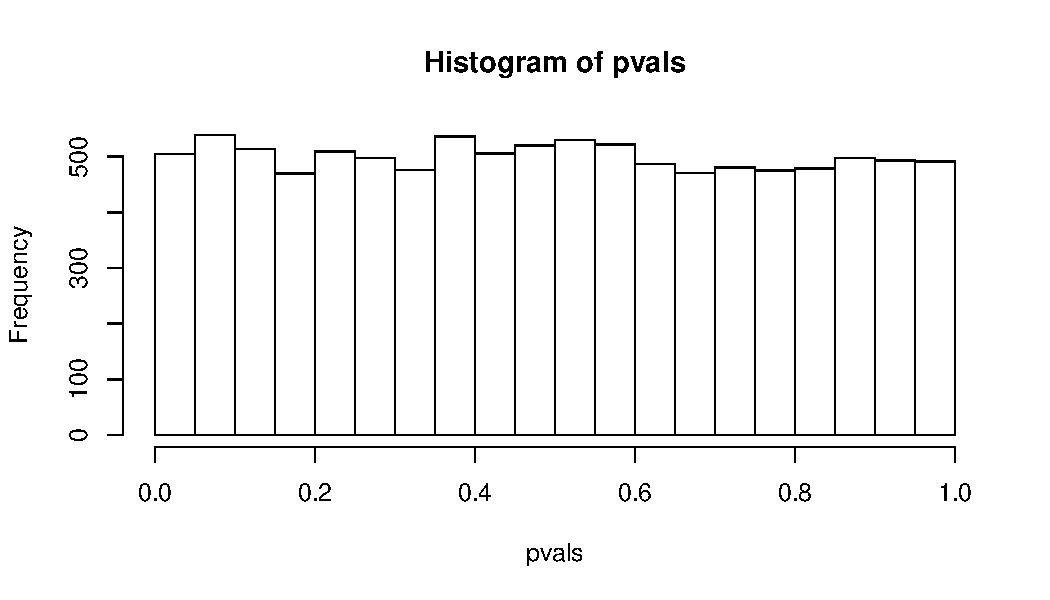
\includegraphics[width=\maxwidth]{figure/unnamed-chunk-117-1} 

\end{knitrout}
\item If the true value of the slope were 0.07 instead of 0.133, what would our power be?

\begin{knitrout}
\definecolor{shadecolor}{rgb}{0.969, 0.969, 0.969}\color{fgcolor}\begin{kframe}
\begin{alltt}
\hlstd{nsim}\hlkwb{<-}\hlnum{10000}
\hlstd{savecoef}\hlkwb{<-}\hlkwd{matrix}\hlstd{(}\hlkwd{rep}\hlstd{(}\hlnum{NA}\hlstd{,nsim}\hlopt{*}\hlnum{2}\hlstd{),}\hlkwc{ncol}\hlstd{=}\hlnum{2}\hlstd{)}
\hlstd{pvals}\hlkwb{<-}\hlkwd{rep}\hlstd{(}\hlnum{NA}\hlstd{,nsim)}
\hlkwa{for}\hlstd{(i} \hlkwa{in} \hlnum{1}\hlopt{:}\hlstd{nsim)\{}
  \hlstd{fakedat}\hlkwb{<-}\hlkwd{gen_fake}\hlstd{(}\hlkwc{slope}\hlstd{=}\hlnum{0.07}\hlstd{)}
  \hlstd{m}\hlkwb{<-}\hlkwd{lm}\hlstd{(eval}\hlopt{~}\hlstd{beauty,fakedat)}
  \hlstd{savecoef[i,]}\hlkwb{<-}\hlstd{m}\hlopt{$}\hlstd{coef}
  \hlstd{pvals[i]}\hlkwb{<-}\hlkwd{summary}\hlstd{(m)}\hlopt{$}\hlstd{coefficient[}\hlnum{2}\hlstd{,}\hlnum{4}\hlstd{]}
\hlstd{\}}
\hlkwd{mean}\hlstd{(pvals}\hlopt{<}\hlnum{0.05}\hlstd{)}
\end{alltt}
\begin{verbatim}
## [1] 0.4111
\end{verbatim}
\end{kframe}
\end{knitrout}

\item In the above scenario where the true value is 0.07, what is the sampling distribution of the mean going to look like? How much overestimation are we going to get in repeated sampling?

\begin{knitrout}
\definecolor{shadecolor}{rgb}{0.969, 0.969, 0.969}\color{fgcolor}\begin{kframe}
\begin{alltt}
\hlkwd{hist}\hlstd{(savecoef[,}\hlnum{2}\hlstd{],}\hlkwc{freq}\hlstd{=}\hlnum{FALSE}\hlstd{,}
     \hlkwc{xlab}\hlstd{=}\hlstr{"estimates"}\hlstd{,}
     \hlkwc{main}\hlstd{=}\hlstr{"Sampling distribution of\textbackslash{}n beauty effect"}\hlstd{)}
\hlkwd{abline}\hlstd{(}\hlkwc{v}\hlstd{=}\hlnum{0.07}\hlstd{,}\hlkwc{col}\hlstd{=}\hlstr{"red"}\hlstd{)}
\end{alltt}
\end{kframe}
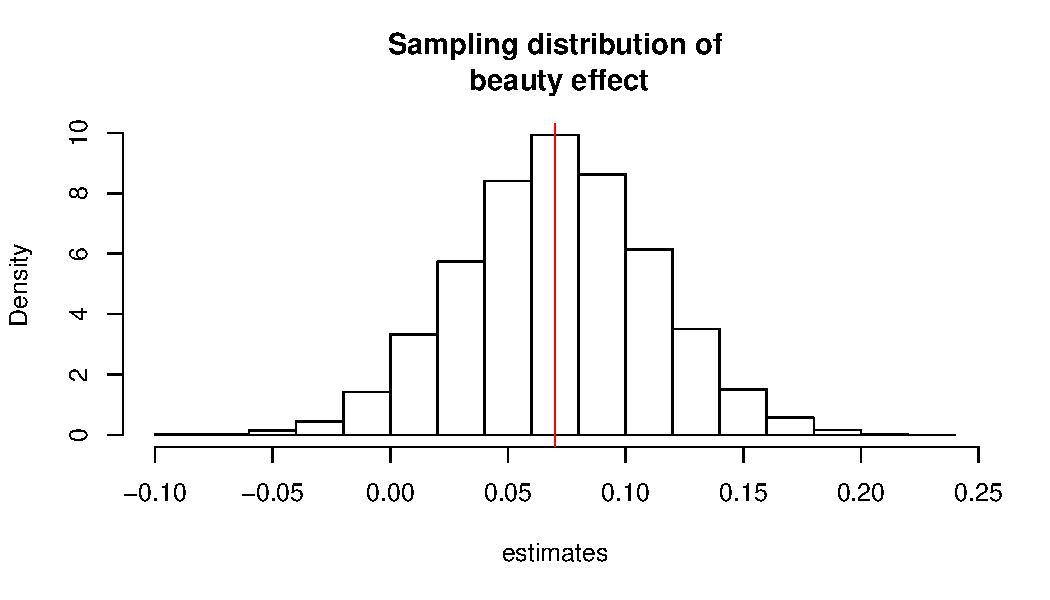
\includegraphics[width=\maxwidth]{figure/unnamed-chunk-119-1} 

\end{knitrout}

\item When power is as low as 40\%, how exaggerated will significant effects be?

\begin{knitrout}
\definecolor{shadecolor}{rgb}{0.969, 0.969, 0.969}\color{fgcolor}\begin{kframe}
\begin{alltt}
\hlkwd{hist}\hlstd{(savecoef[,}\hlnum{2}\hlstd{][}\hlkwd{which}\hlstd{(pvals}\hlopt{<}\hlnum{0.05}\hlstd{)],}\hlkwc{xlab}\hlstd{=}\hlstr{"estimate"}\hlstd{,}\hlkwc{freq}\hlstd{=}\hlnum{FALSE}\hlstd{,}\hlkwc{main}\hlstd{=}\hlstr{"Type M error with 40% power"}\hlstd{)}
\hlkwd{abline}\hlstd{(}\hlkwc{v}\hlstd{=}\hlnum{0.07}\hlstd{,}\hlkwc{col}\hlstd{=}\hlstr{"red"}\hlstd{)}
\end{alltt}
\end{kframe}
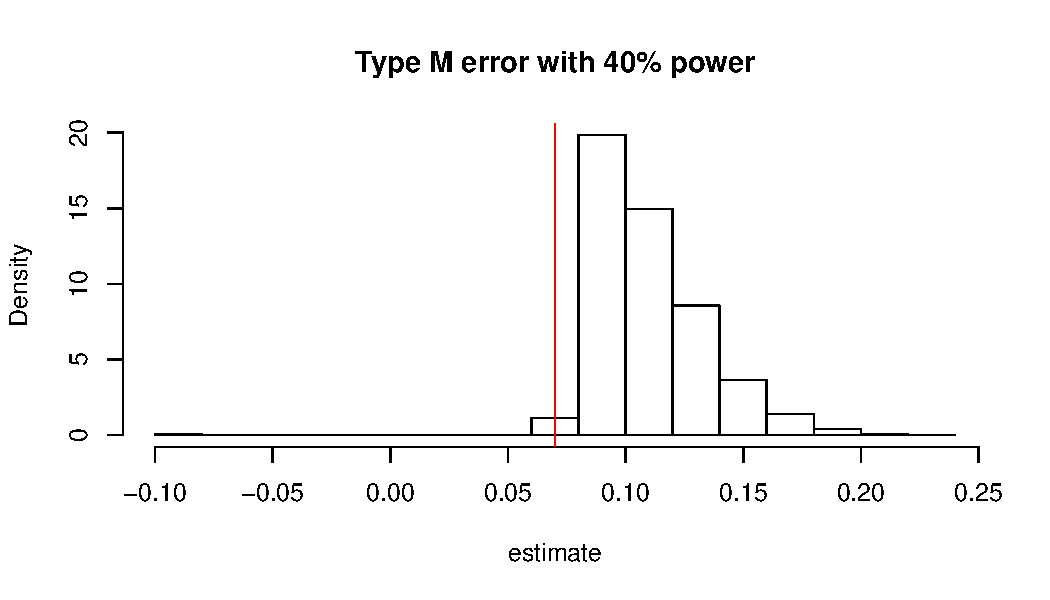
\includegraphics[width=\maxwidth]{figure/unnamed-chunk-120-1} 

\end{knitrout}

\end{enumerate}

In the next chapter, fake data simulation will prove very helpful in evaluating how realistic the model is, and whether we have any reasonable chance of detecting accurate estimates of an effect.



%\include{appendix}


\backmatter%%%%%%%%%%%%%%%%%%%%%%%%%%%%%%%%%%%%%%%%%%%%%%%%%%%%%%%
%\include{glossary}
%\include{solutions}
%\printindex

%%%%%%%%%%%%%%%%%%%%%%%%%%%%%%%%%%%%%%%%%%%%%%%%%%%%%%%%%%%%%%%%%%%%%%

\bibliographystyle{plain}
\bibliography{/Users/shravanvasishth/Dropbox/Bibliography/bibcleaned}

\end{document}





